\chapter{Application: Cardiac Mechanics}
%

\begin{figure}[ht]
\centering
\subfigure[]{%
		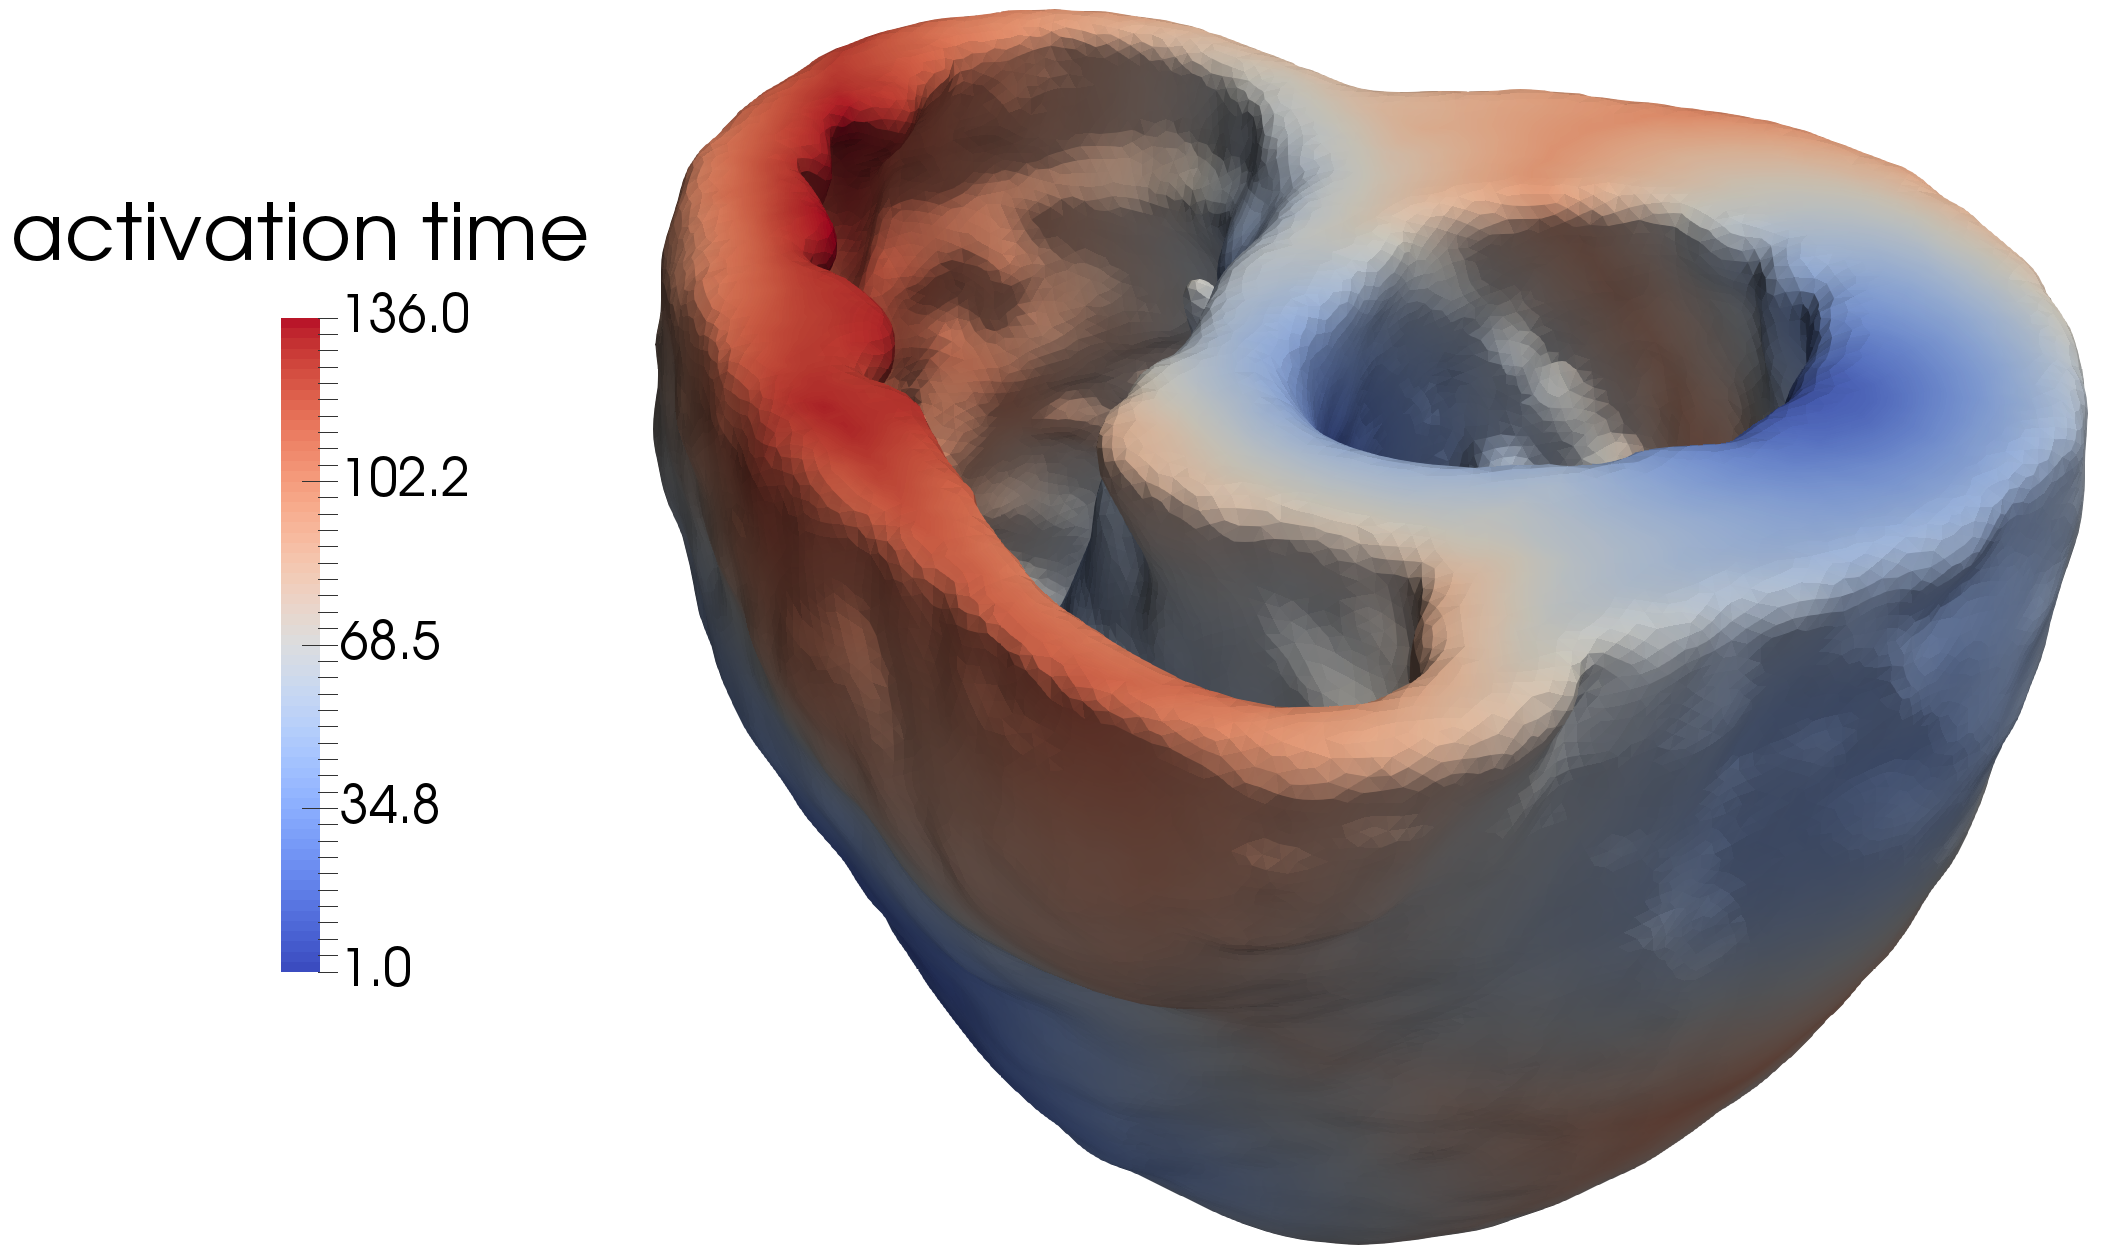
\includegraphics[scale=0.081]{media/4-cardioid/2-activationtime.png}
\label{fig:supp1}}
\subfigure[]{%
		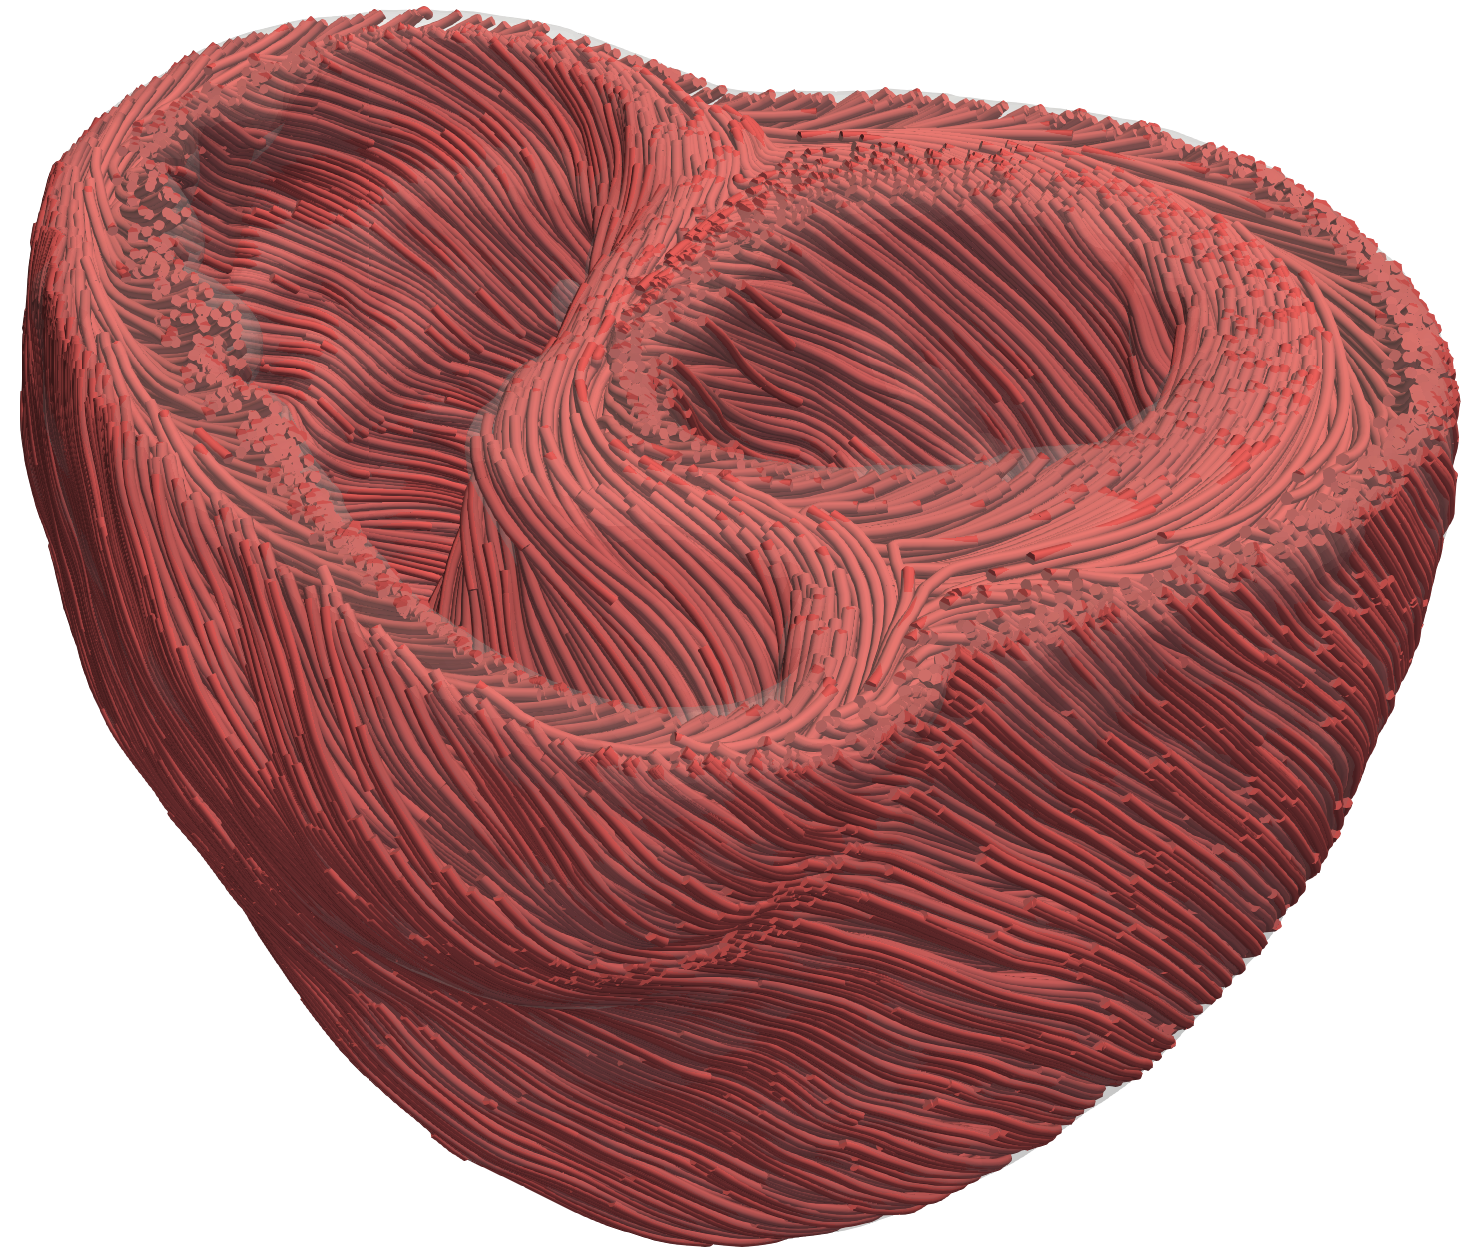
\includegraphics[scale=0.081]{media/4-cardioid/3-fibers.png}
\label{fig:supp2}}
\subfigure[]{%
		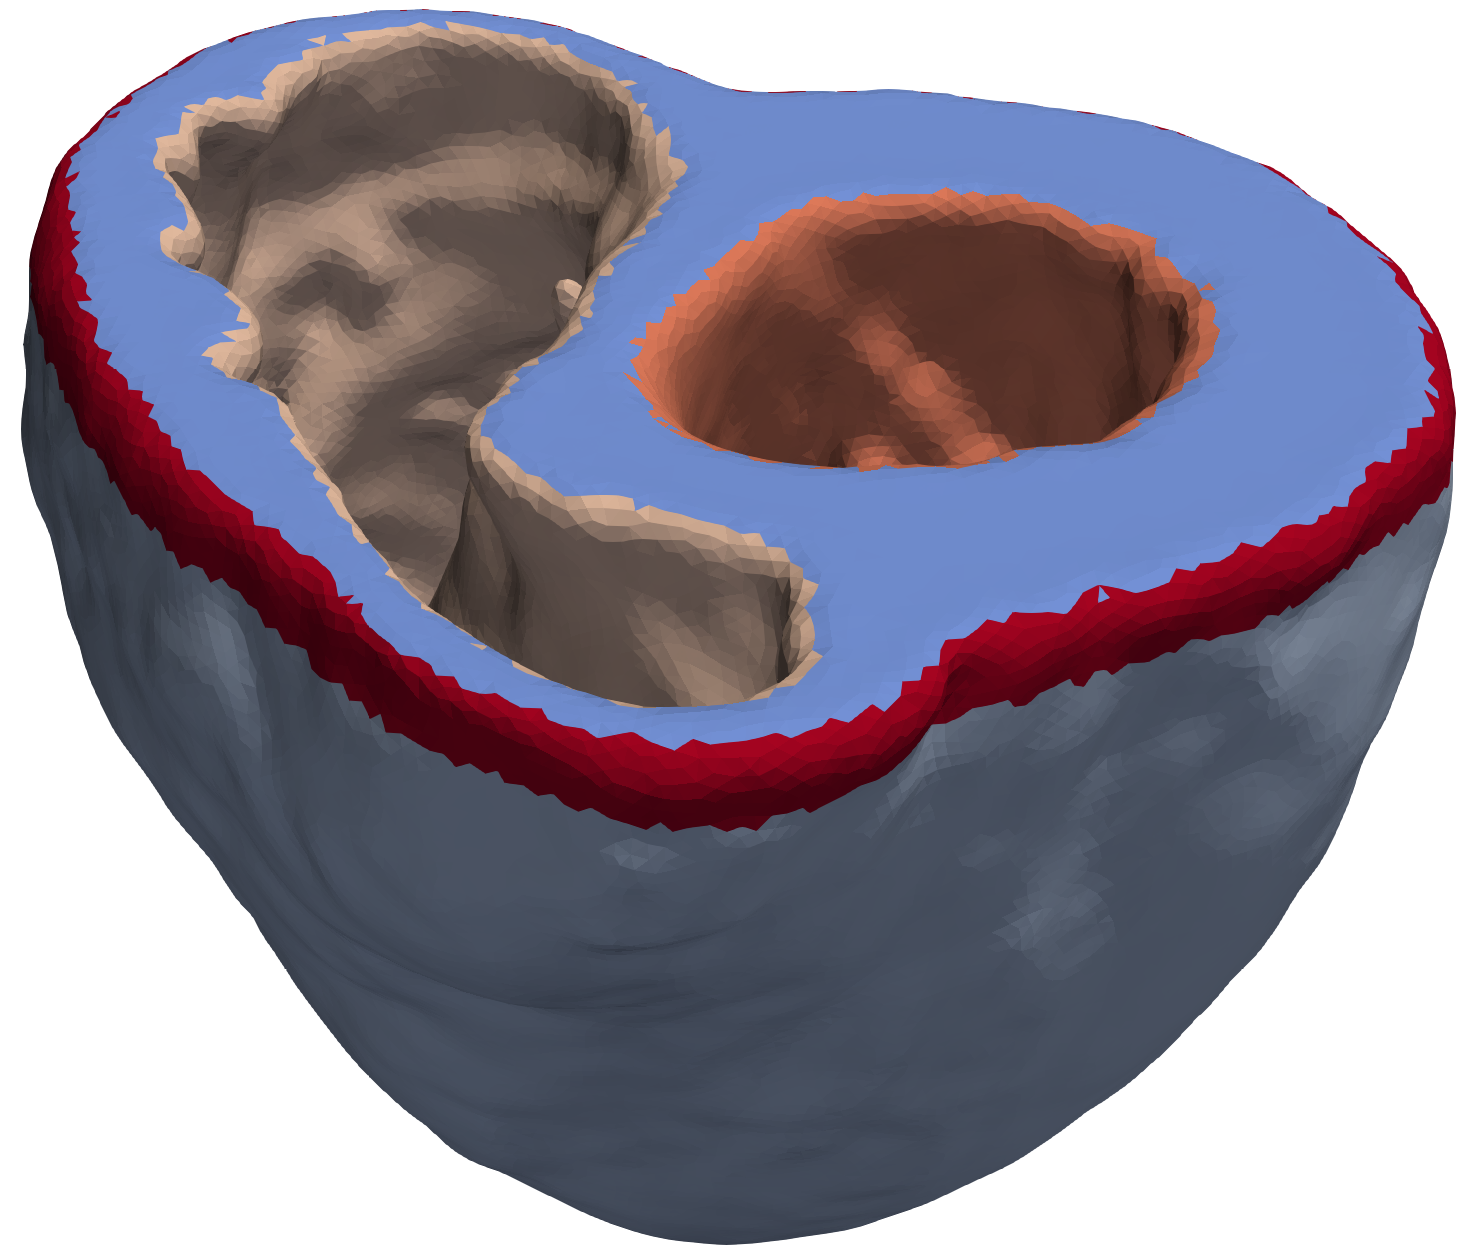
\includegraphics[scale=0.081]{media/4-cardioid/4-tagged.png}
\label{fig:supp3}}
%
\caption{Mechanics modeling considerations: (a) muscle fiber orientations, (b) electrical activation times, and c) surface tagging and prescription of corresponding boundary conditions.}
\label{fig:supp}
\end{figure}

\begin{figure}[ht]
\centering
\subfigure[]{%
		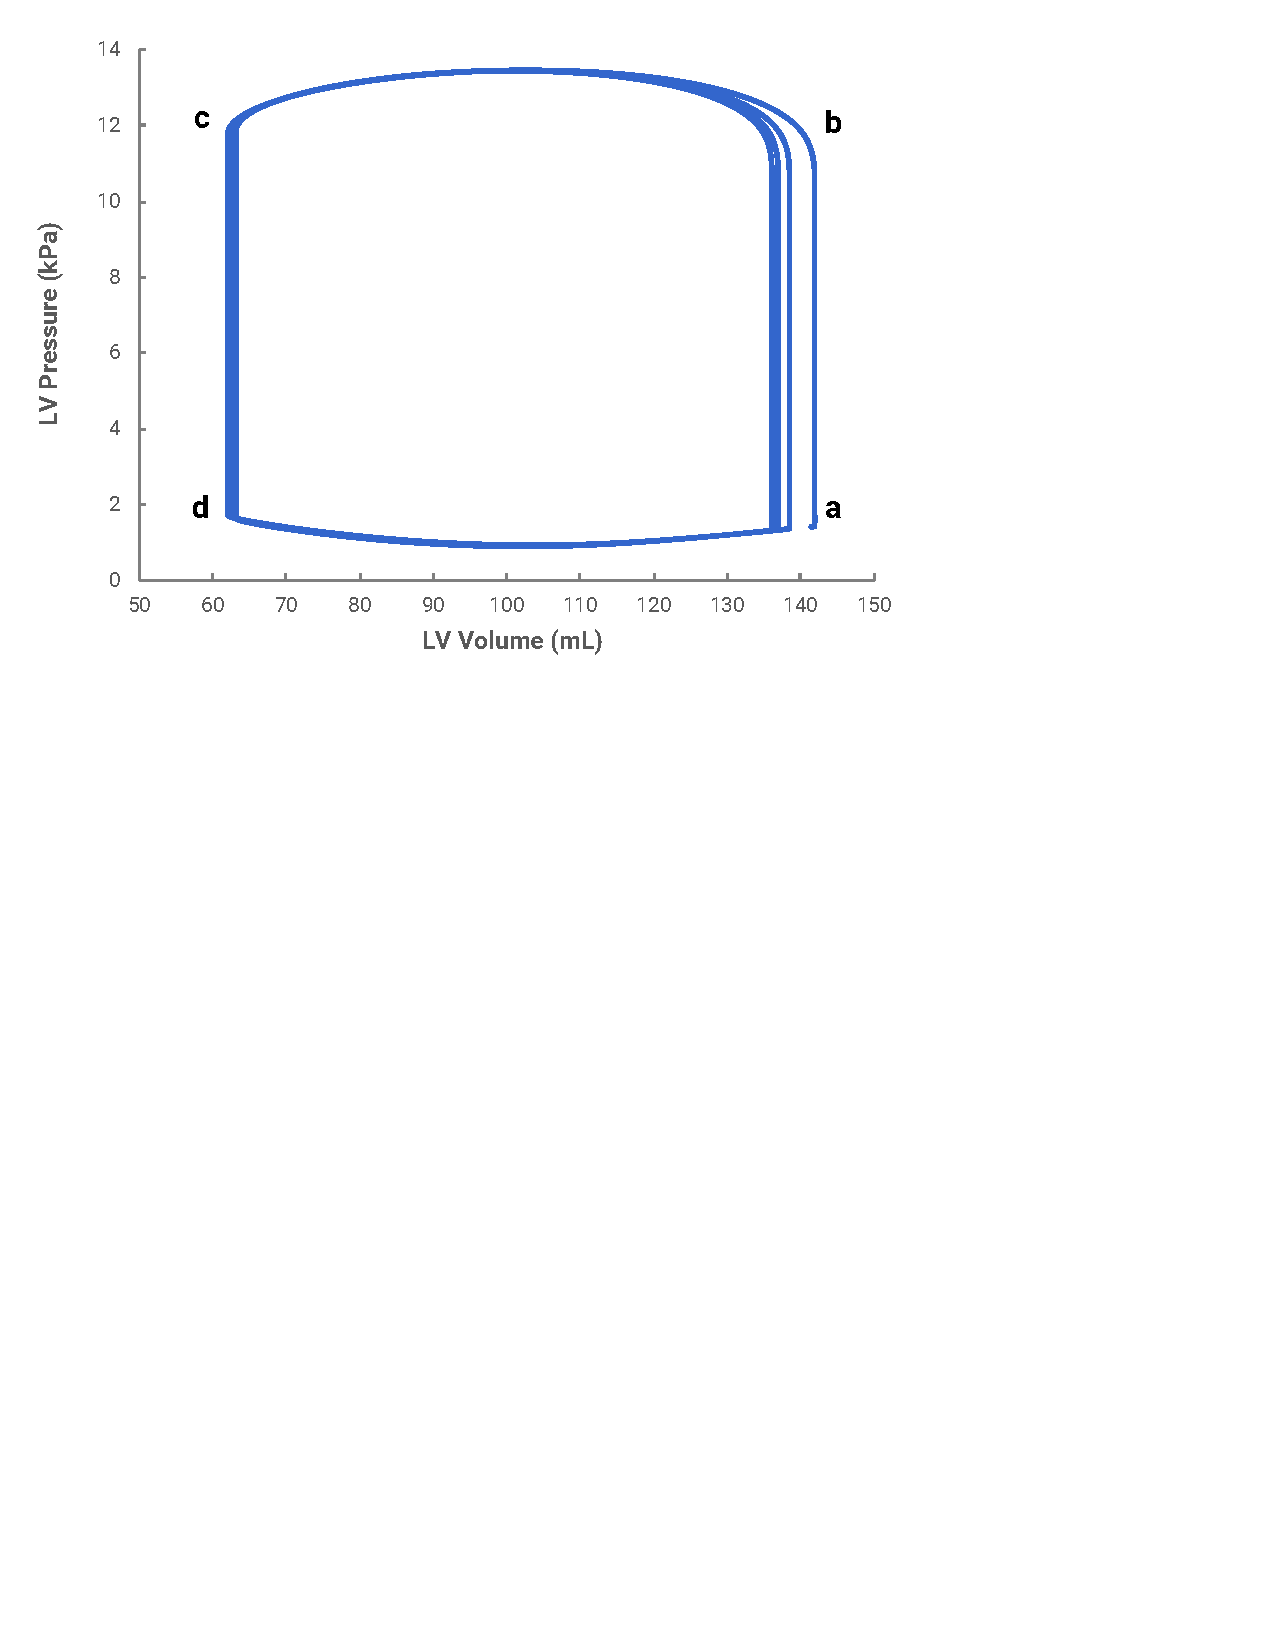
\includegraphics[scale=0.5]{media/4-cardioid/5-pv/pressure_volume-1.pdf}
\label{fig:pv1}}		
\subfigure[]{%
		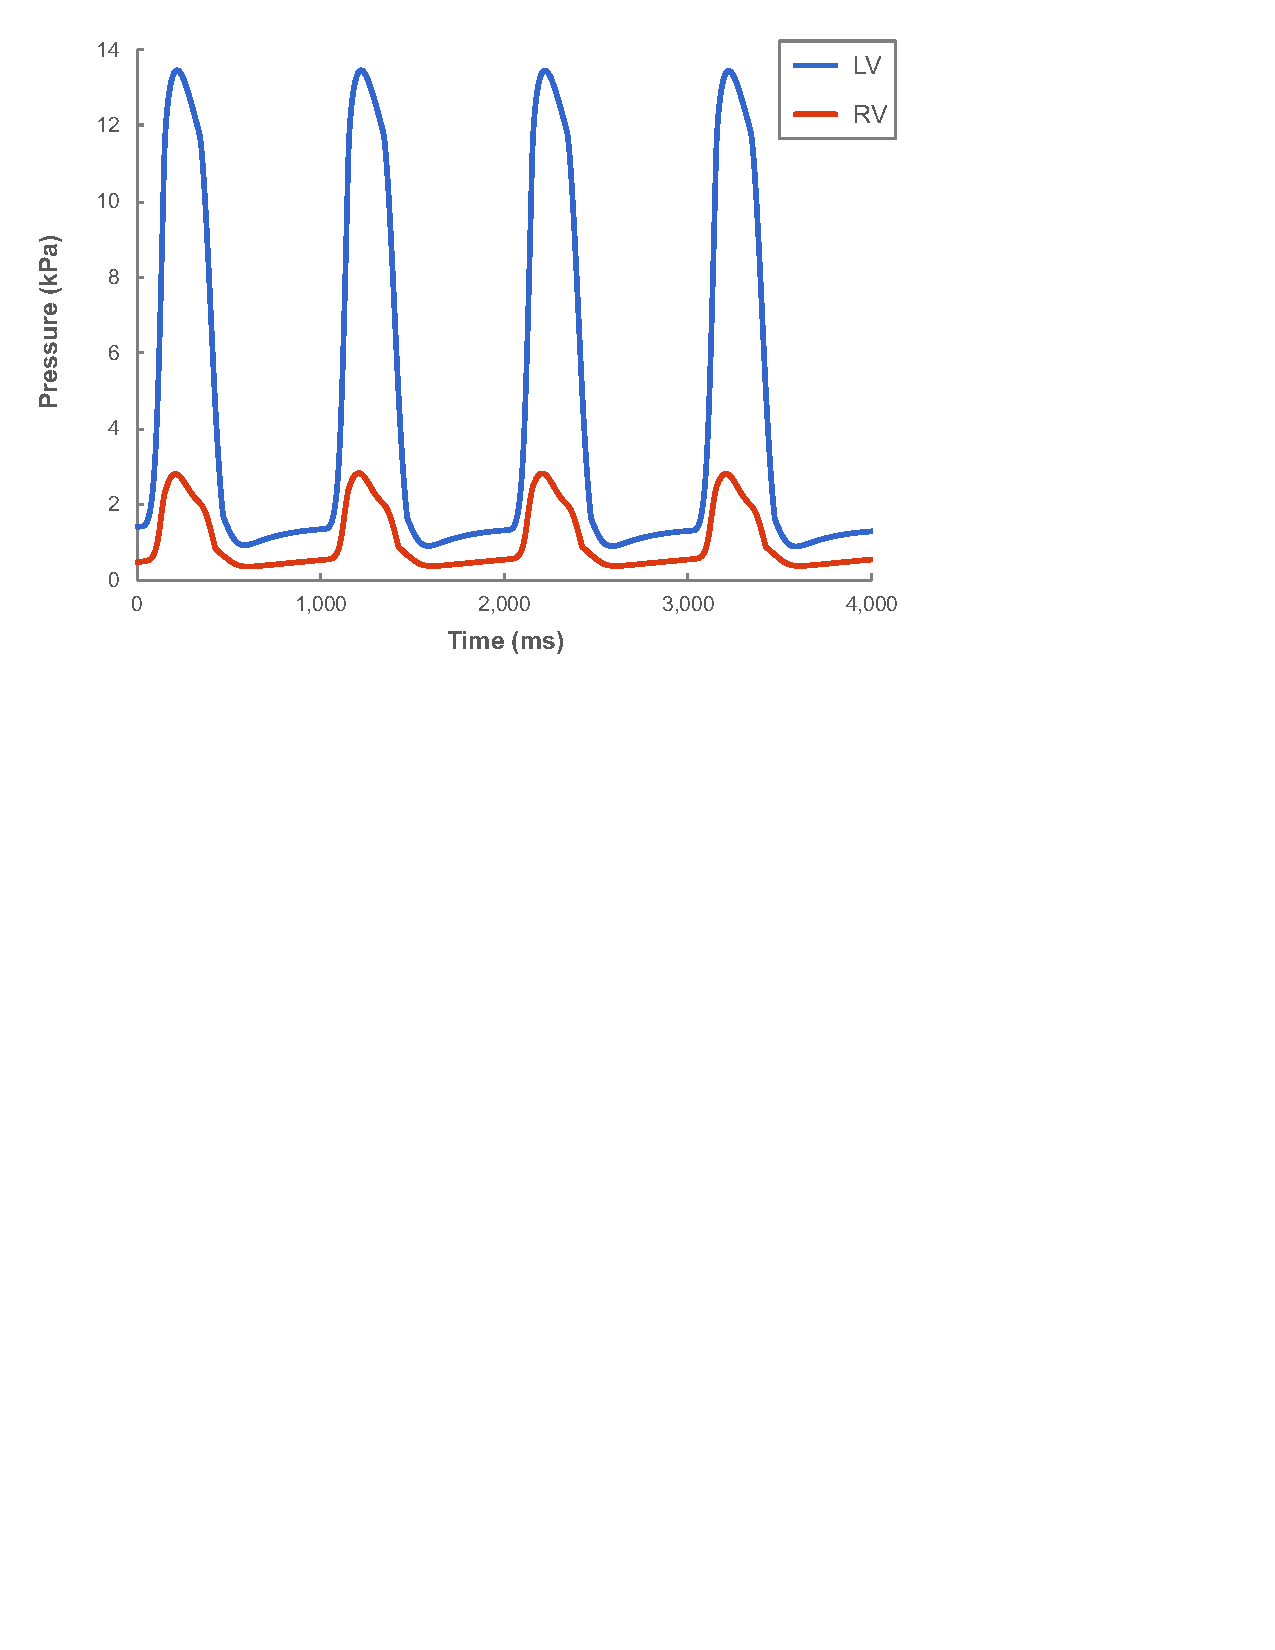
\includegraphics[scale=0.5]{media/4-cardioid/5-pv/pressure_volume-2.pdf}
\label{fig:pv2}}		
%
\caption{Results from Cardioid simulation: (a) P-V loop of left ventricle, (b) pressure time history in left and right ventricles.}
\label{fig:pv}
\end{figure}

\begin{figure}[ht!]
\centering
\subfigure[]{%
		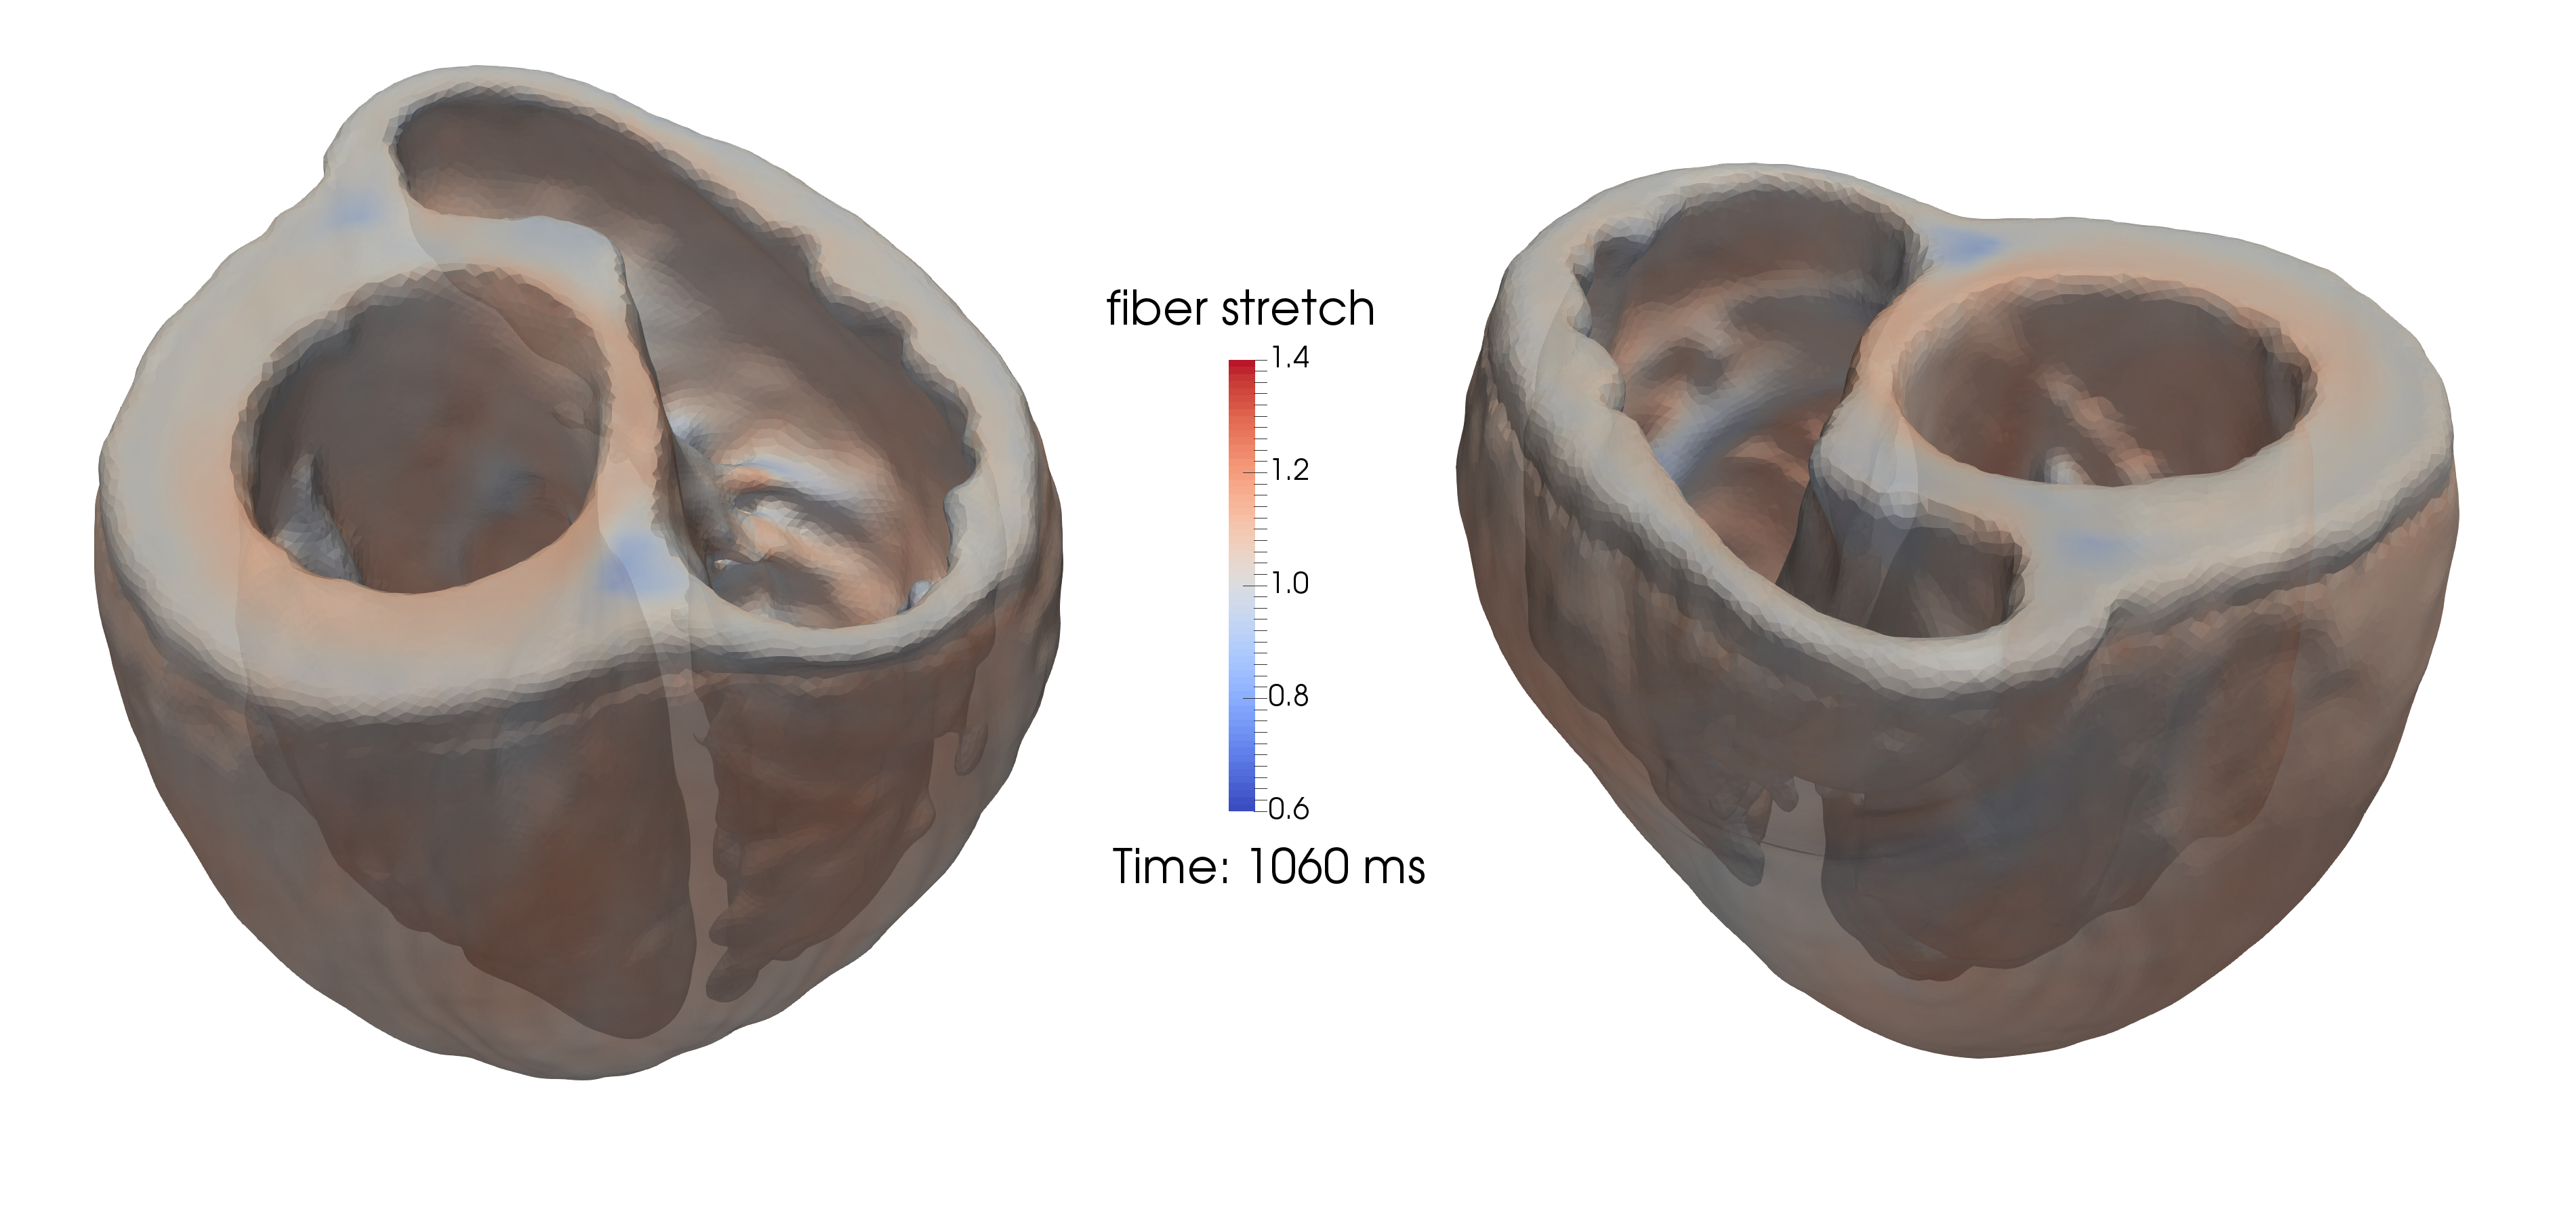
\includegraphics[scale=0.057]{media/4-cardioid/6-vid/a.png}
\label{fig:snaps1}}		
\subfigure[]{%
		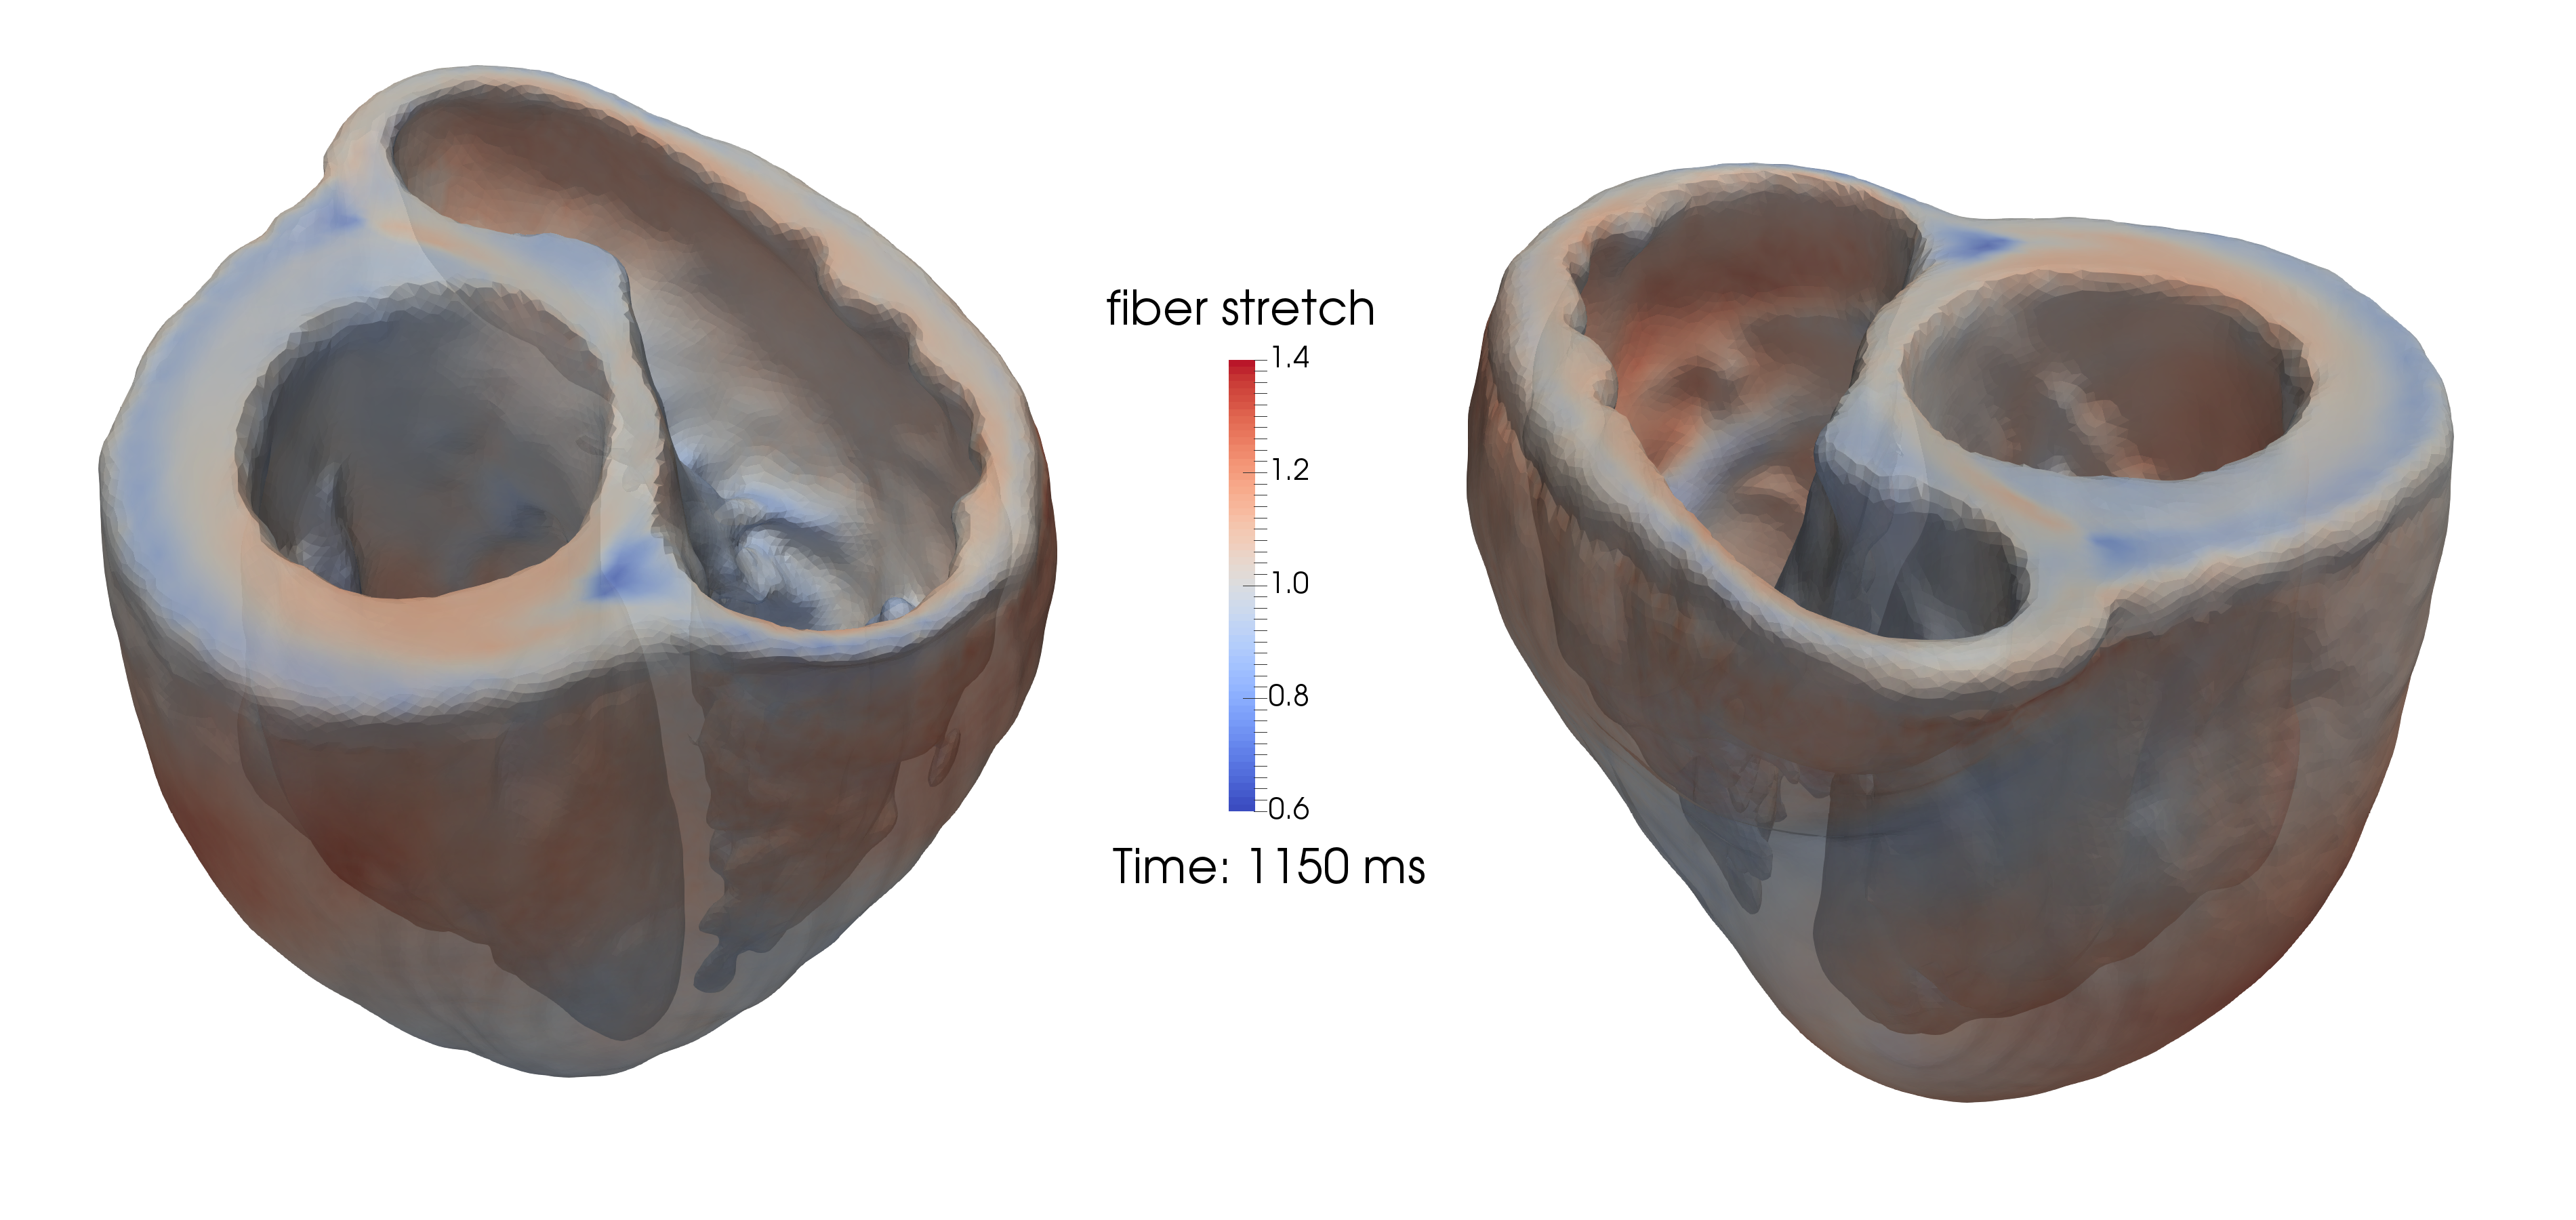
\includegraphics[scale=0.057]{media/4-cardioid/6-vid/b.png}
\label{fig:snaps2}}		
\subfigure[]{%
		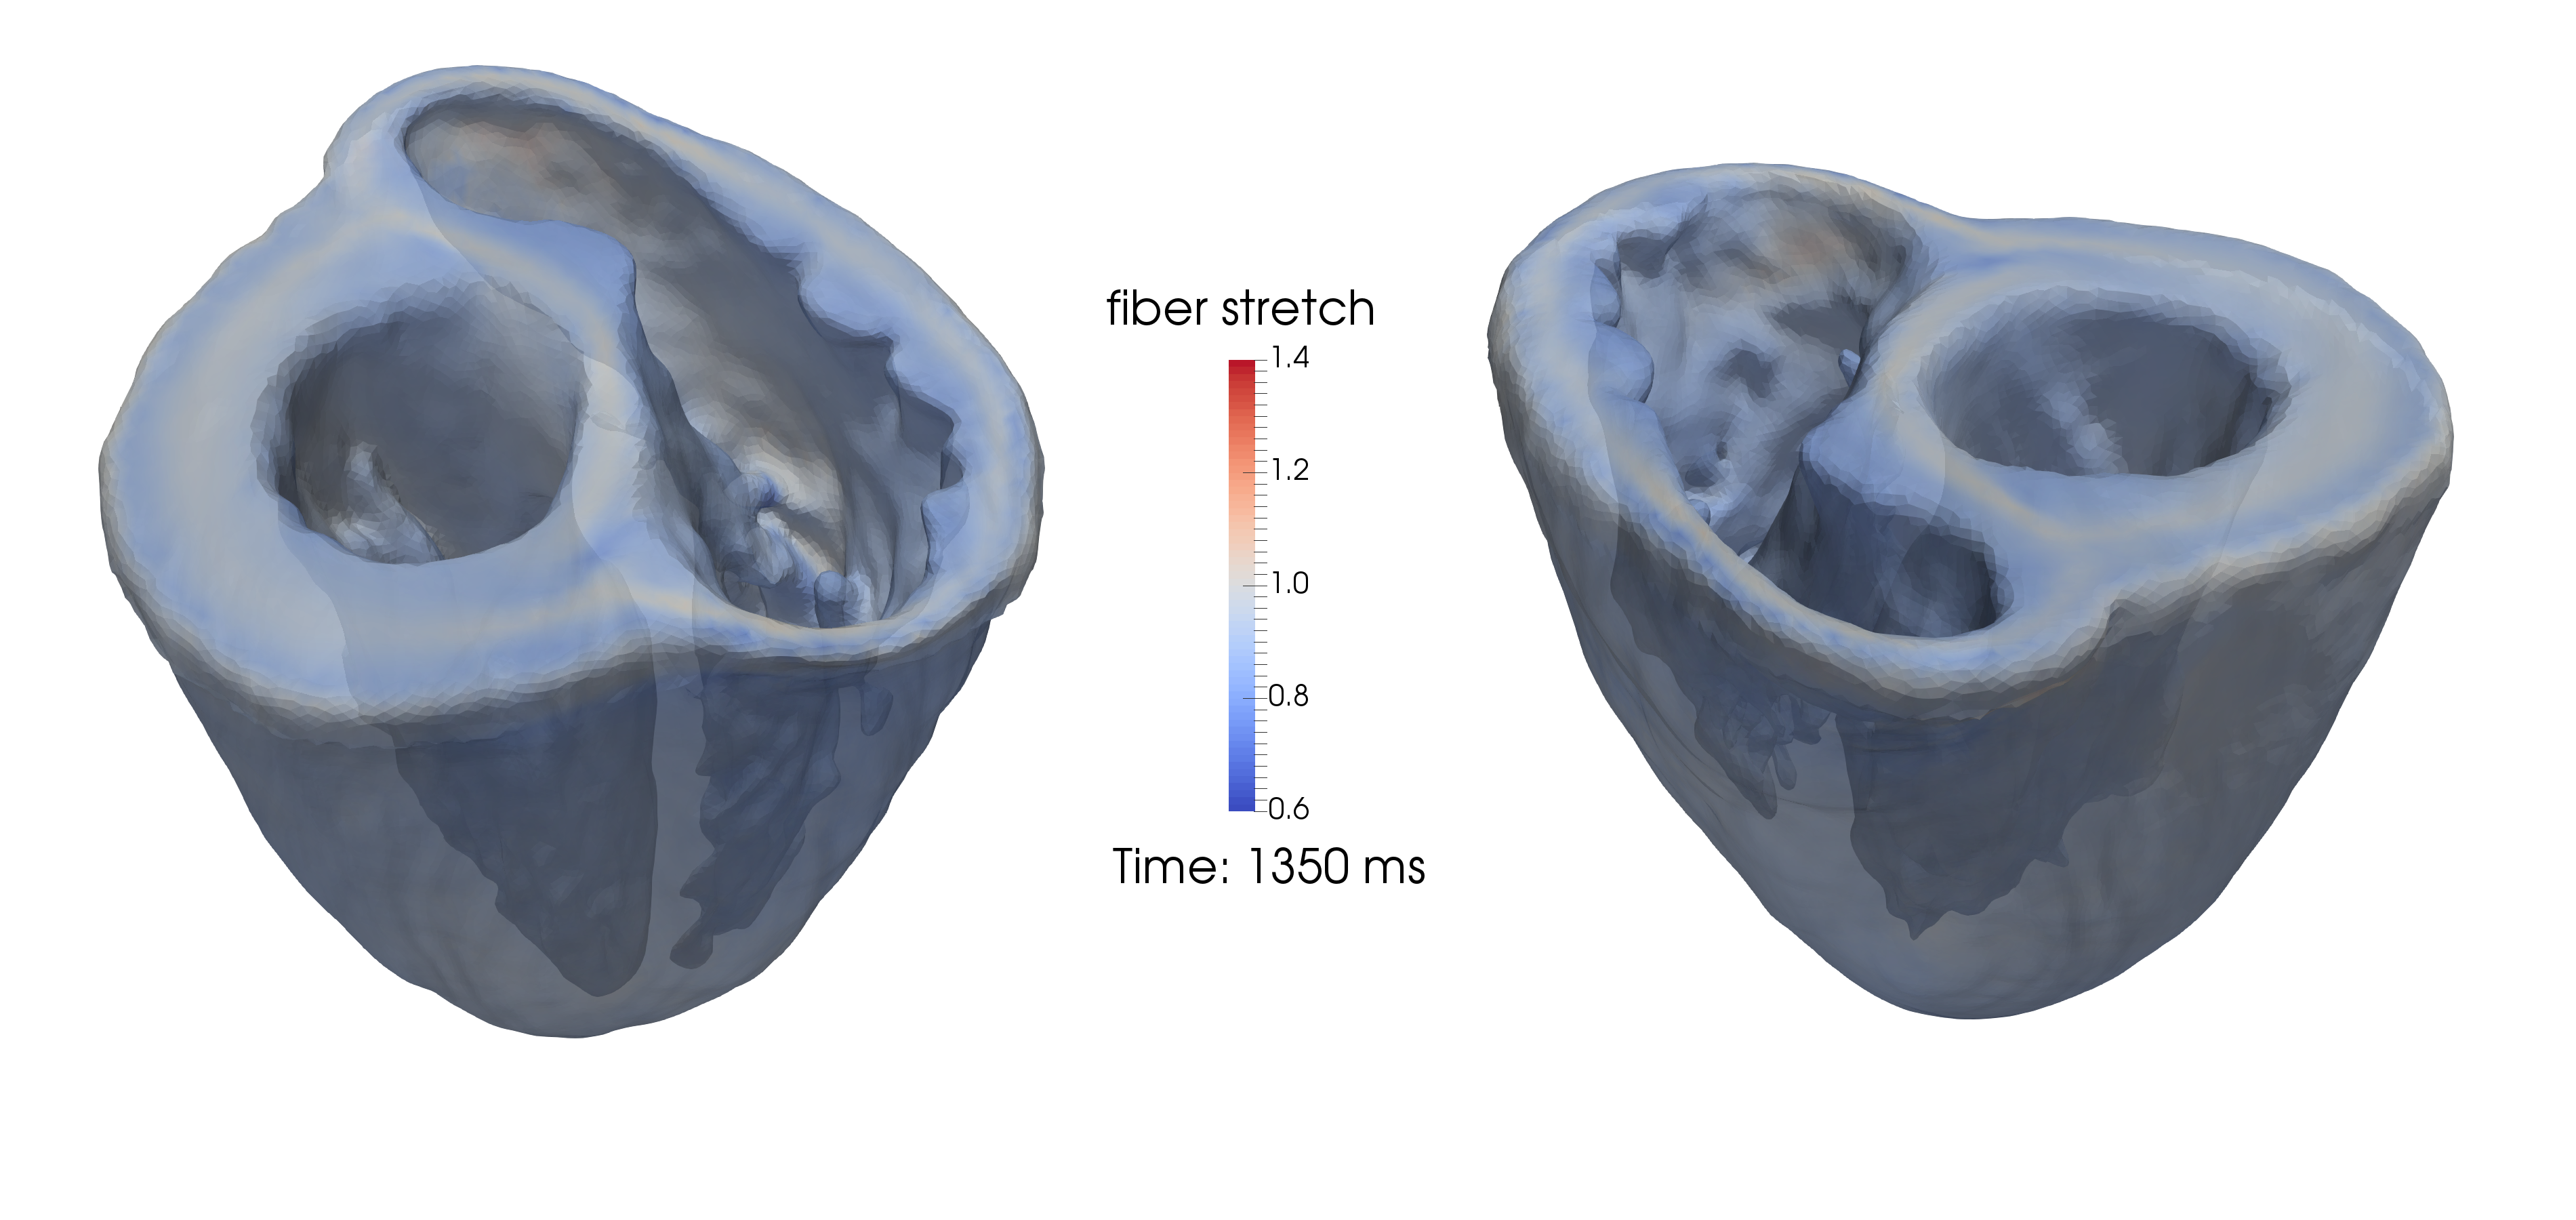
\includegraphics[scale=0.057]{media/4-cardioid/6-vid/c.png}
\label{fig:snapsf3}}		
\subfigure[]{%
		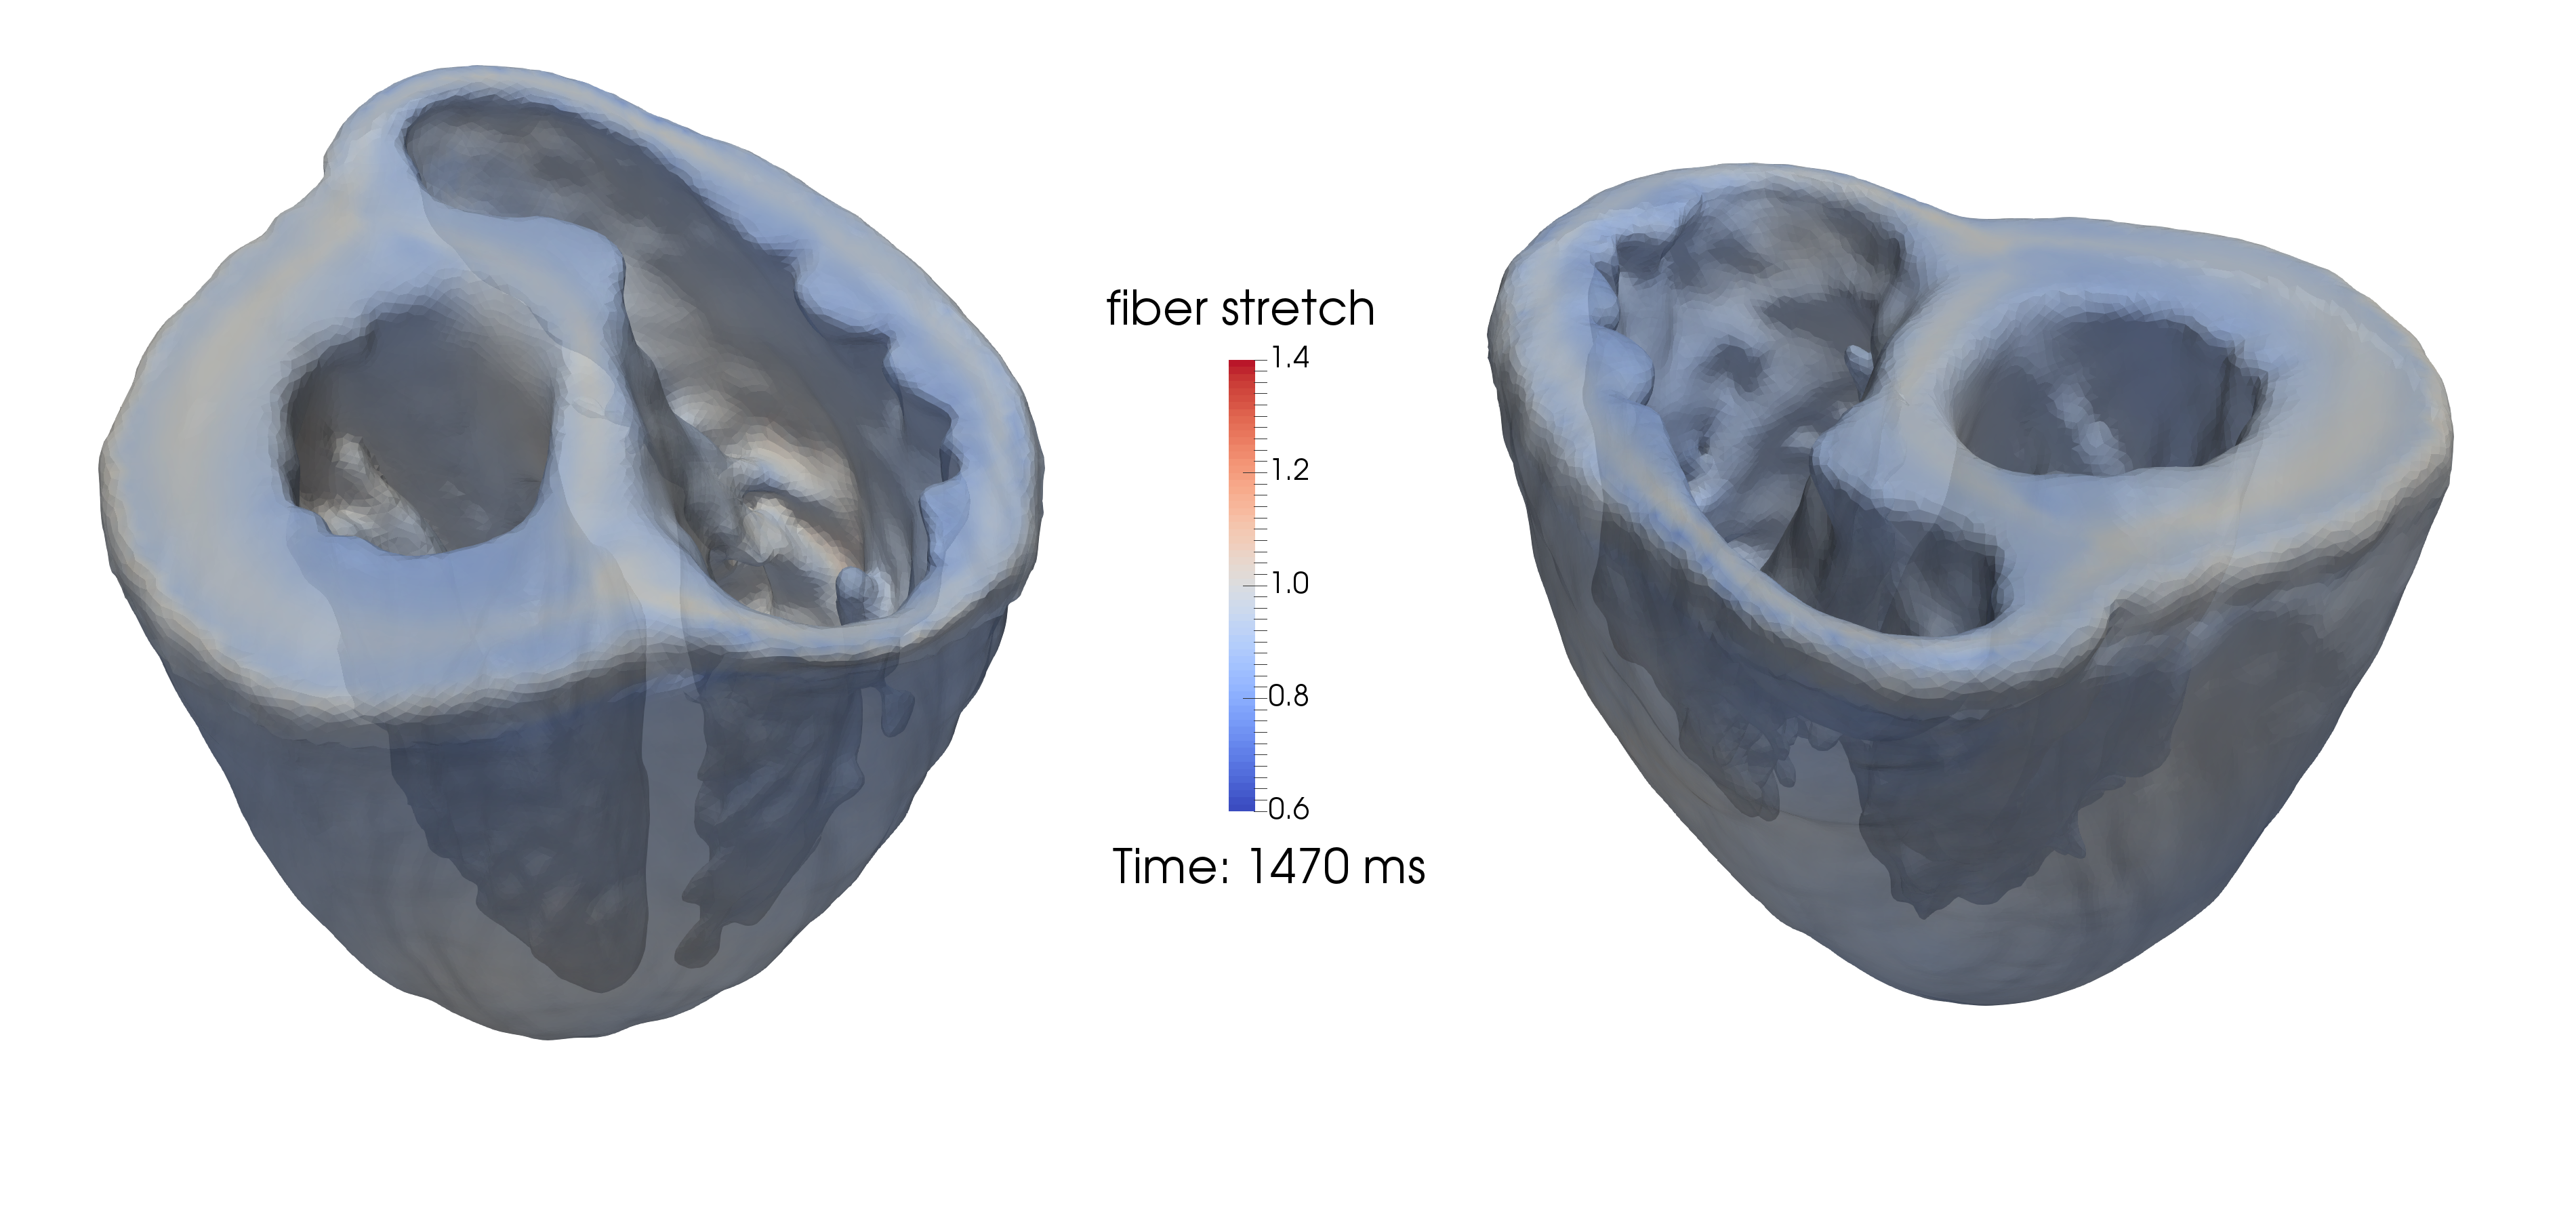
\includegraphics[scale=0.057]{media/4-cardioid/6-vid/d.png}
\label{fig:snaps4}}		
%
\caption{Deformed mesh from Cardioid simulation at different stages of cardiac cycle. Panels (a), (b), (c), and (d) correspond to the stages in the P-V loop denoted in FIGREF ???.}
\label{fig:snaps}
\end{figure}

\begin{figure}[ht]
\centering
\subfigure[]{%
		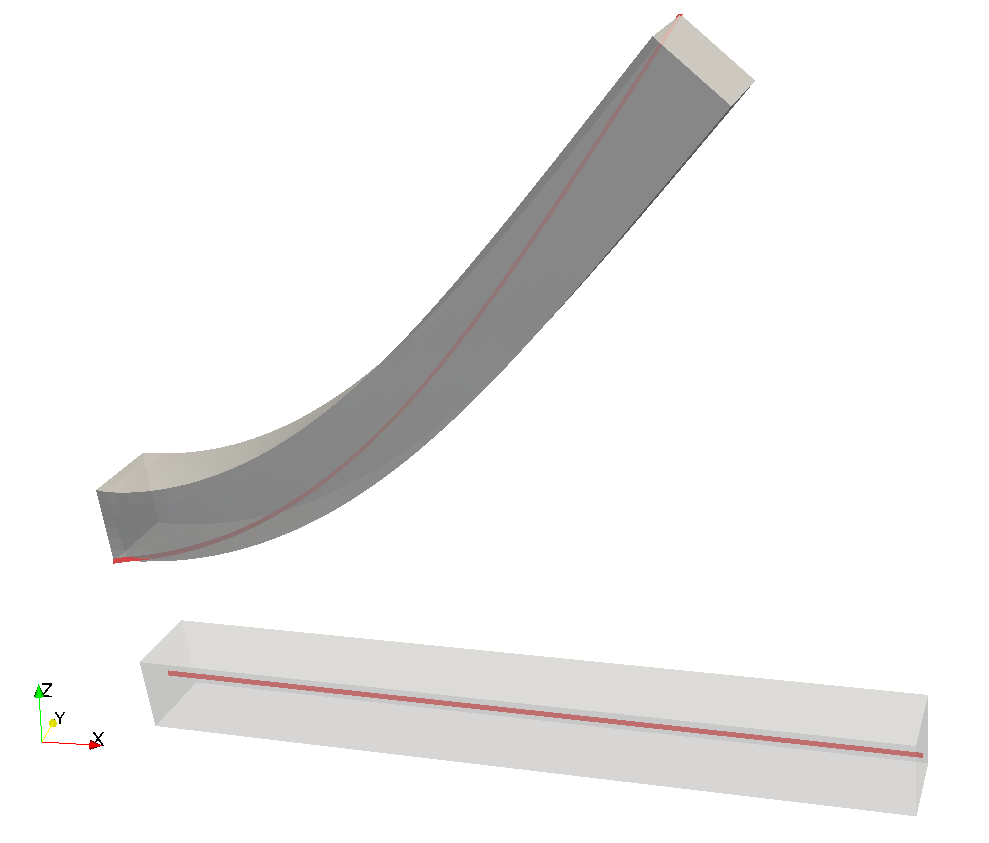
\includegraphics[scale=0.18]{media/5-verif/1-gurev2/gurev2.png}
\label{fig:beams1}}		
\subfigure[]{%
		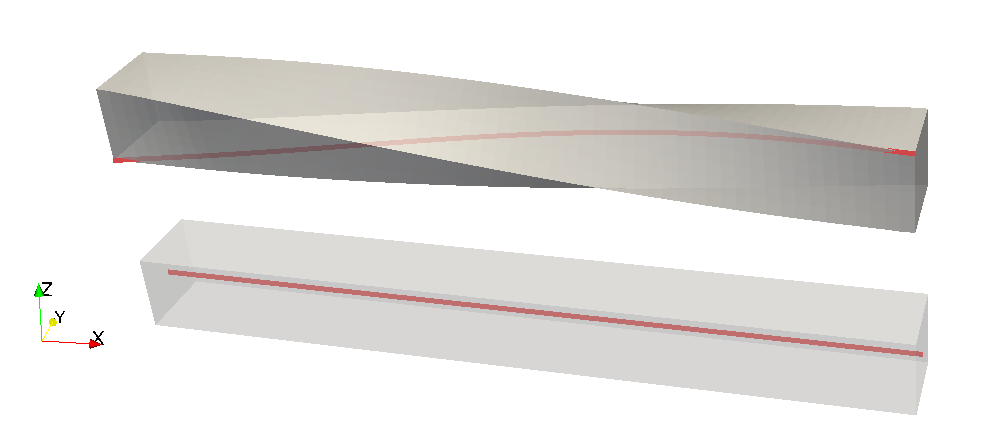
\includegraphics[scale=0.18]{media/5-verif/2-gurev3/gurev3.png}
\label{fig:beams2}}		
\subfigure[]{%
		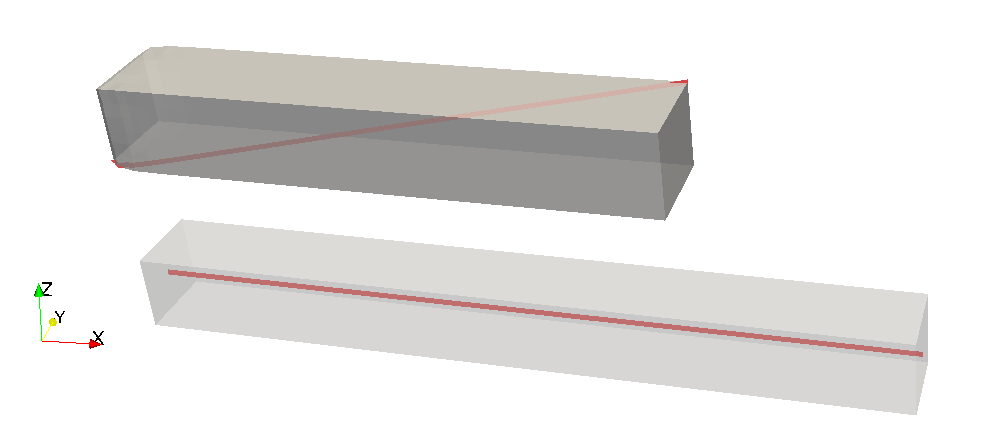
\includegraphics[scale=0.18]{media/5-verif/3-gurev4/gurev4.png}
\label{fig:beams3}}		
\subfigure[]{%
		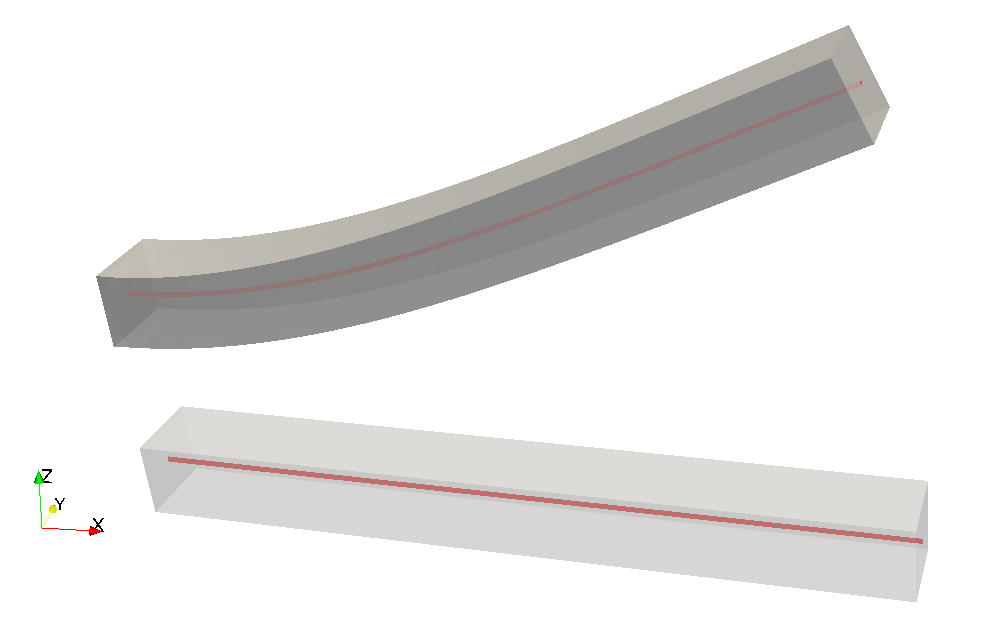
\includegraphics[scale=0.18]{media/5-verif/4-land1/land1.png}
\label{fig:beams4}}		
%
\caption{Undeformed (bottom) and deformed (top) configurations for cantilever beam verification problems: (a) Gurev P2: bending, (b) Gurev P3: torsion, c) Gurev P4: active contraction, and (d) Land P1: bending. The red curve denotes the curve over which displacements and positions are recorded for comparison of results.}
\label{fig:beams}
\end{figure}

\begin{figure}[ht]
\centering
\subfigure[]{%
		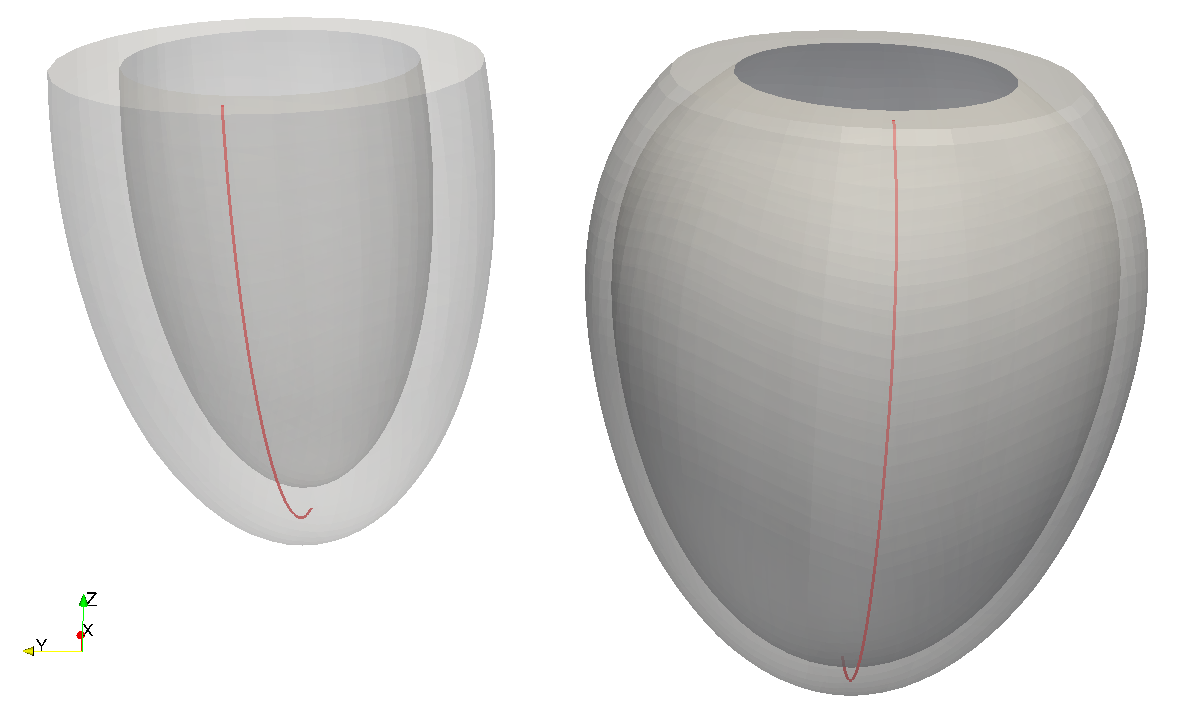
\includegraphics[scale=0.18]{media/5-verif/5-land2/land2-1.png}
\label{fig:ventricles1}}		
\subfigure[]{%
		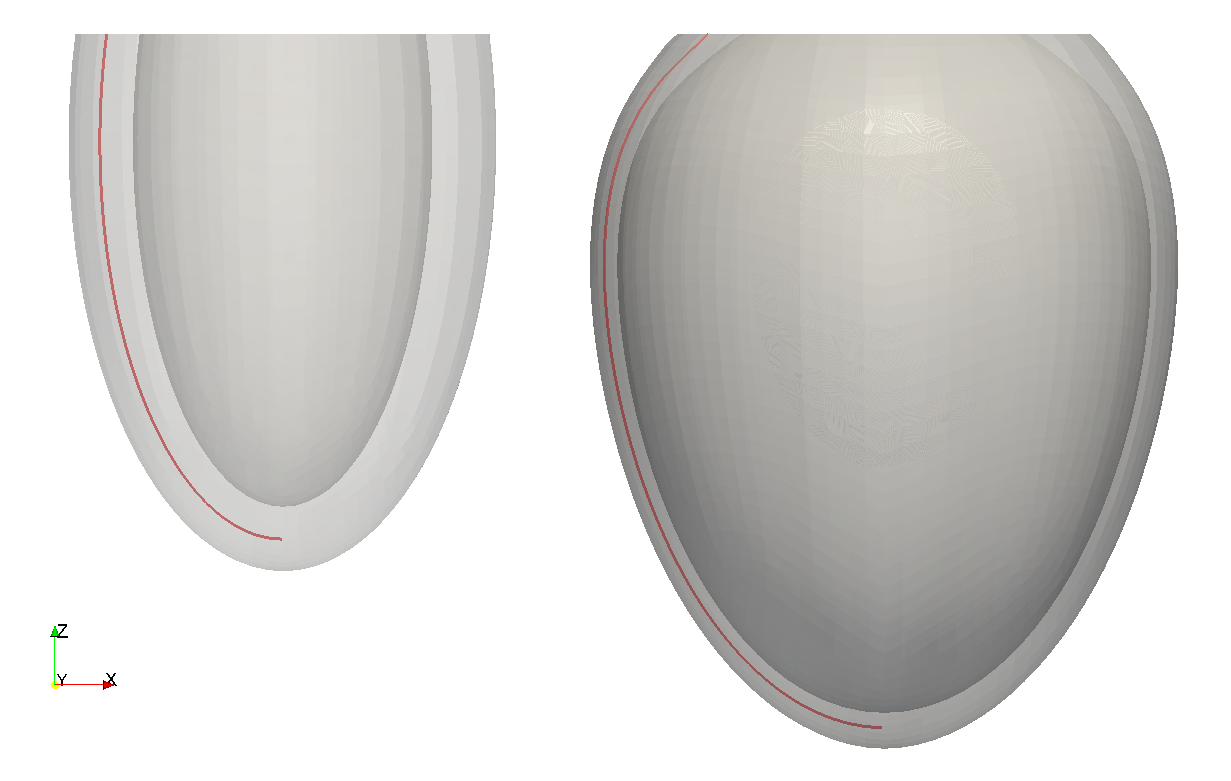
\includegraphics[scale=0.18]{media/5-verif/5-land2/land2-2.png}
\label{fig:ventricles2}}		
\subfigure[]{%
		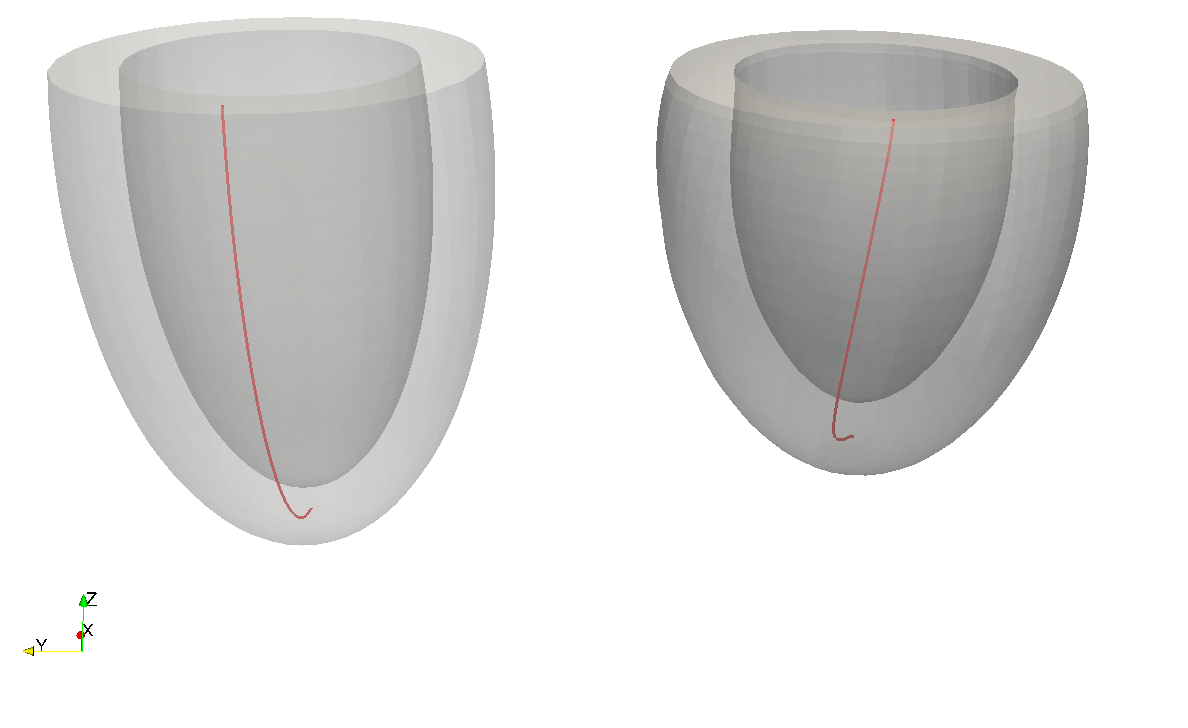
\includegraphics[scale=0.18]{media/5-verif/6-land3/land3-1.png}
\label{fig:ventricles3}}		
\subfigure[]{%
		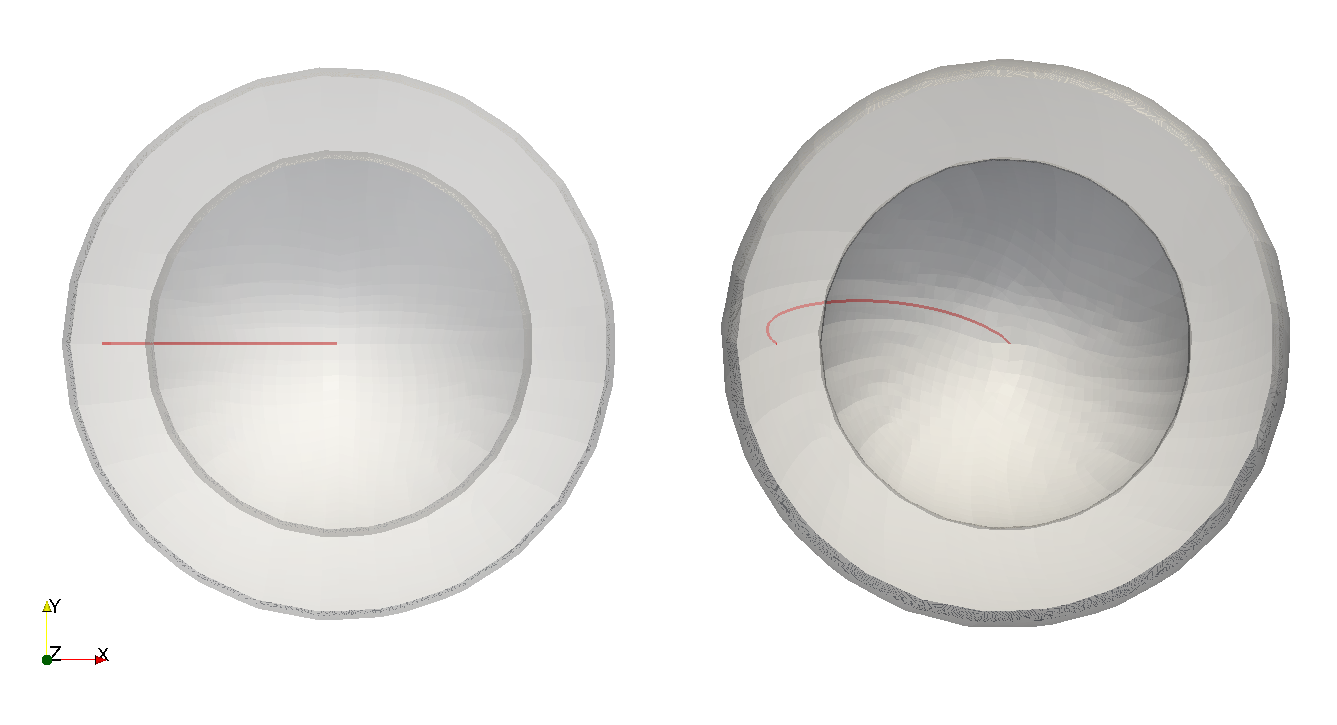
\includegraphics[scale=0.16]{media/5-verif/6-land3/land3-2.png}
\label{fig:ventricles4}}		
%
\caption{Undeformed (left) and deformed (right) configurations for single ventricle verification problems: (a,b) Land P2: inflation, and (c,d) Land P3: inflation and active contraction. The red curve denotes the curve over which displacements and positions are recorded for comparison of results.}
\label{fig:ventricles}
\end{figure}

\begin{figure}[ht]
\centering
\subfigure[]{%
		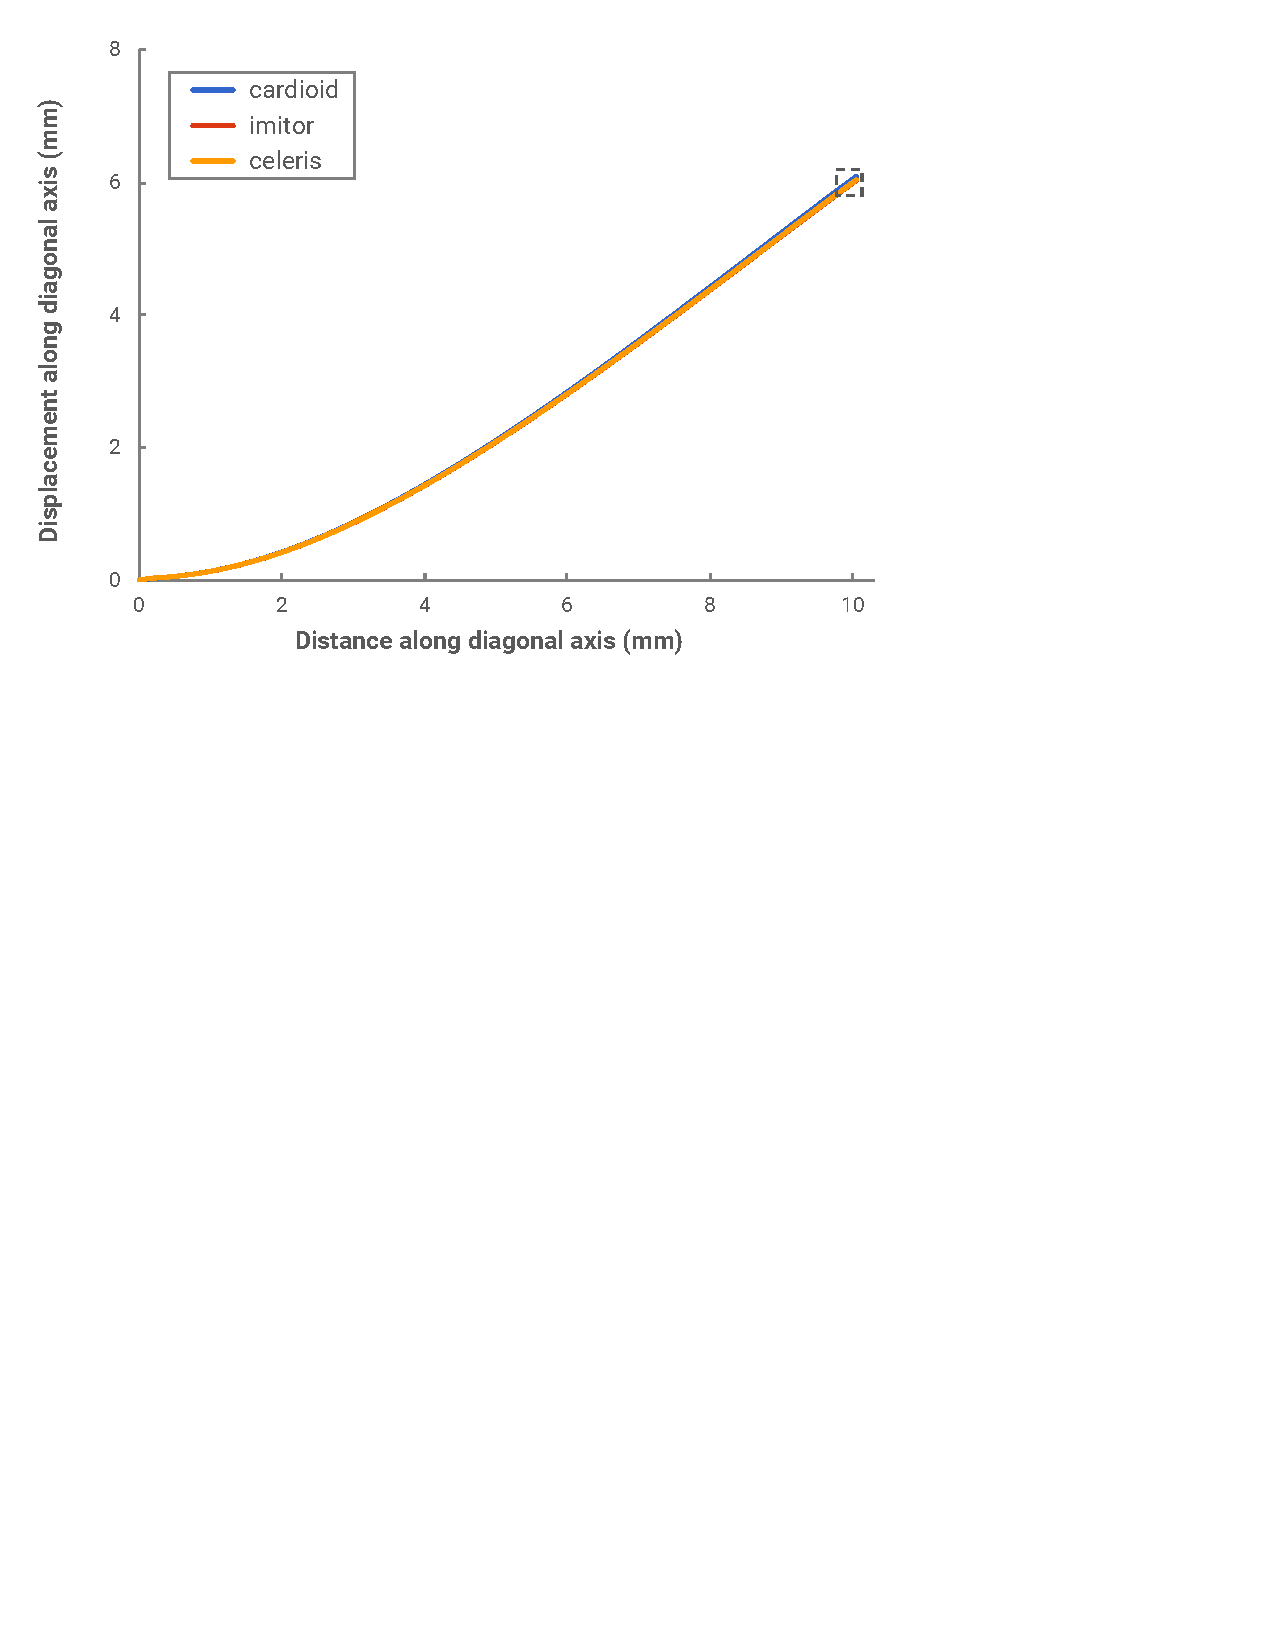
\includegraphics[scale=0.5]{media/5-verif/1-gurev2/gurev2-1.pdf}
\label{fig:gurev2-1}}		
\subfigure[]{%
		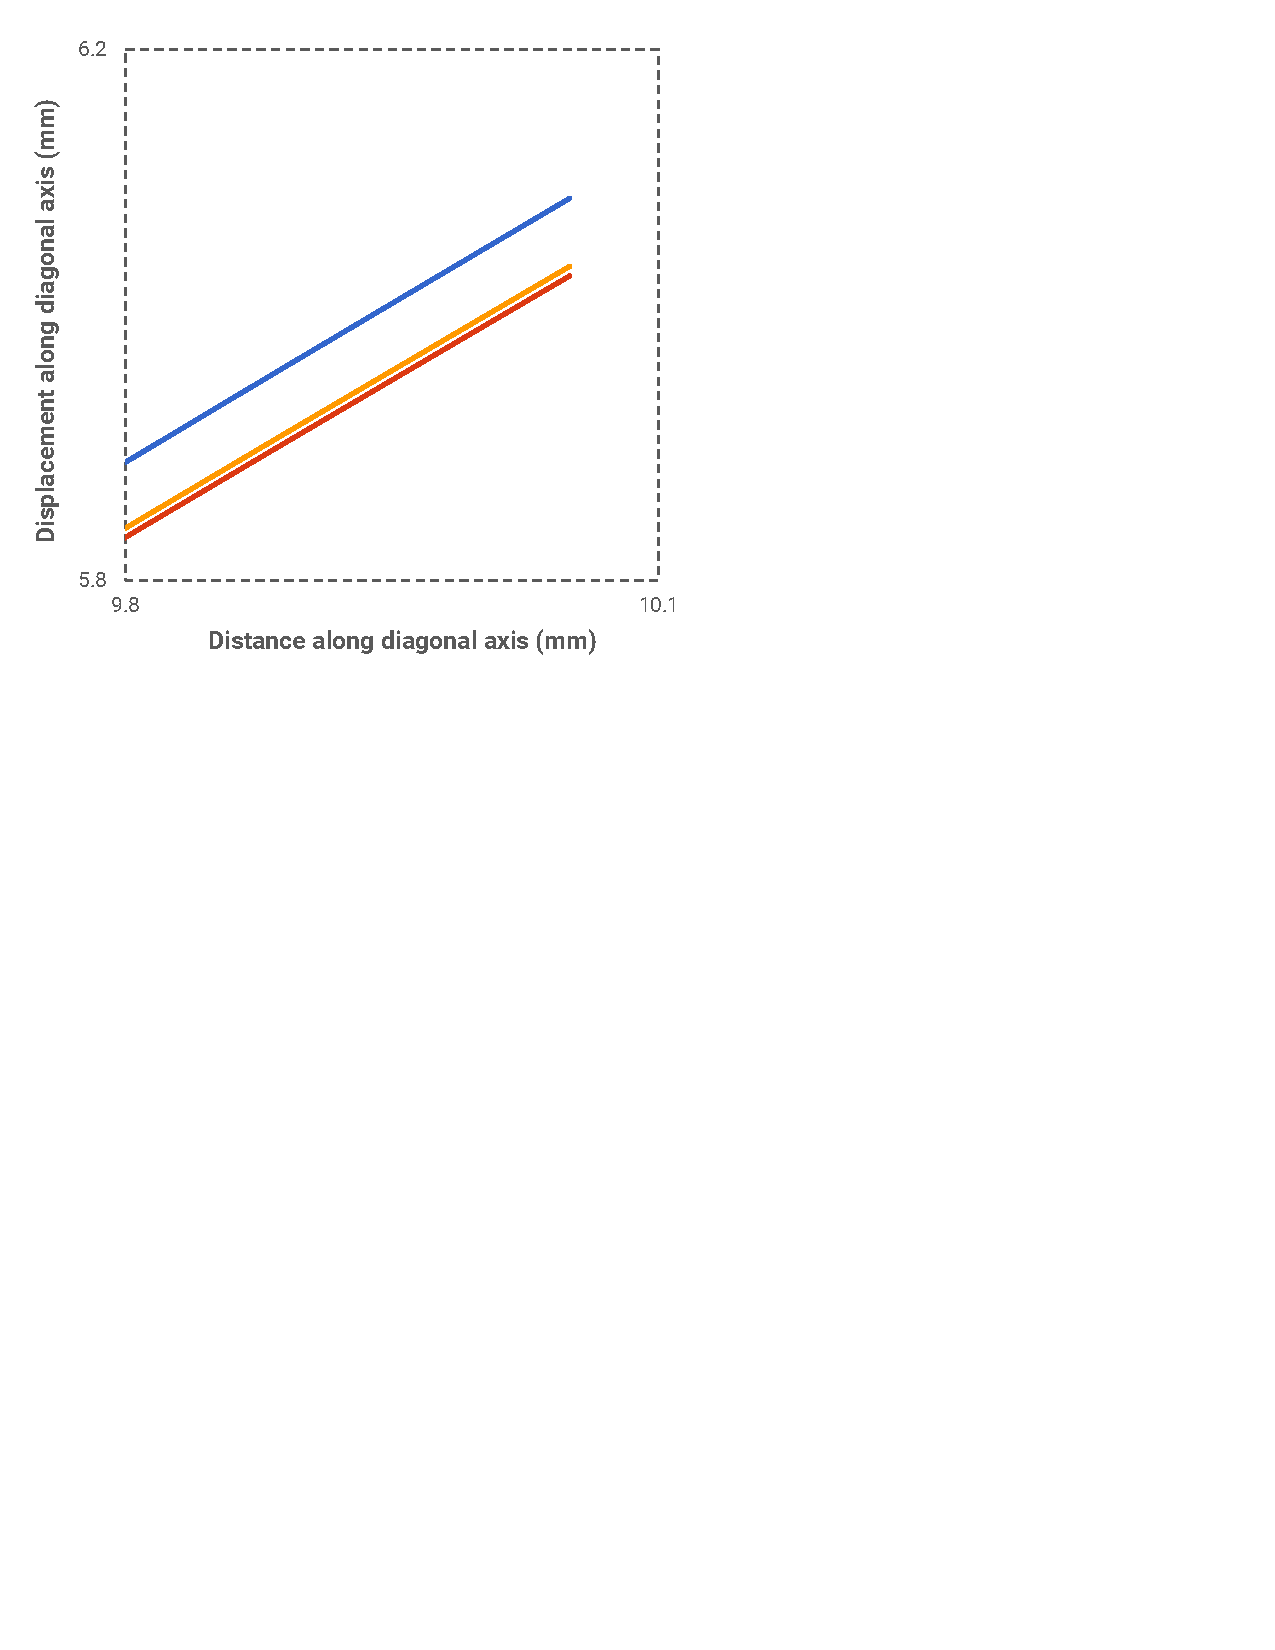
\includegraphics[scale=0.5]{media/5-verif/1-gurev2/gurev2-2.pdf}
\label{fig:gurev2-2}}		
%
\caption{Results for Gurev P2 verification problem: (a) Displacement magnitude along diagonal axis, with (b) details for the free end of the beam}
\label{fig:gurev2}
\end{figure}

\begin{figure}[ht!]
\centering
\subfigure[]{%
		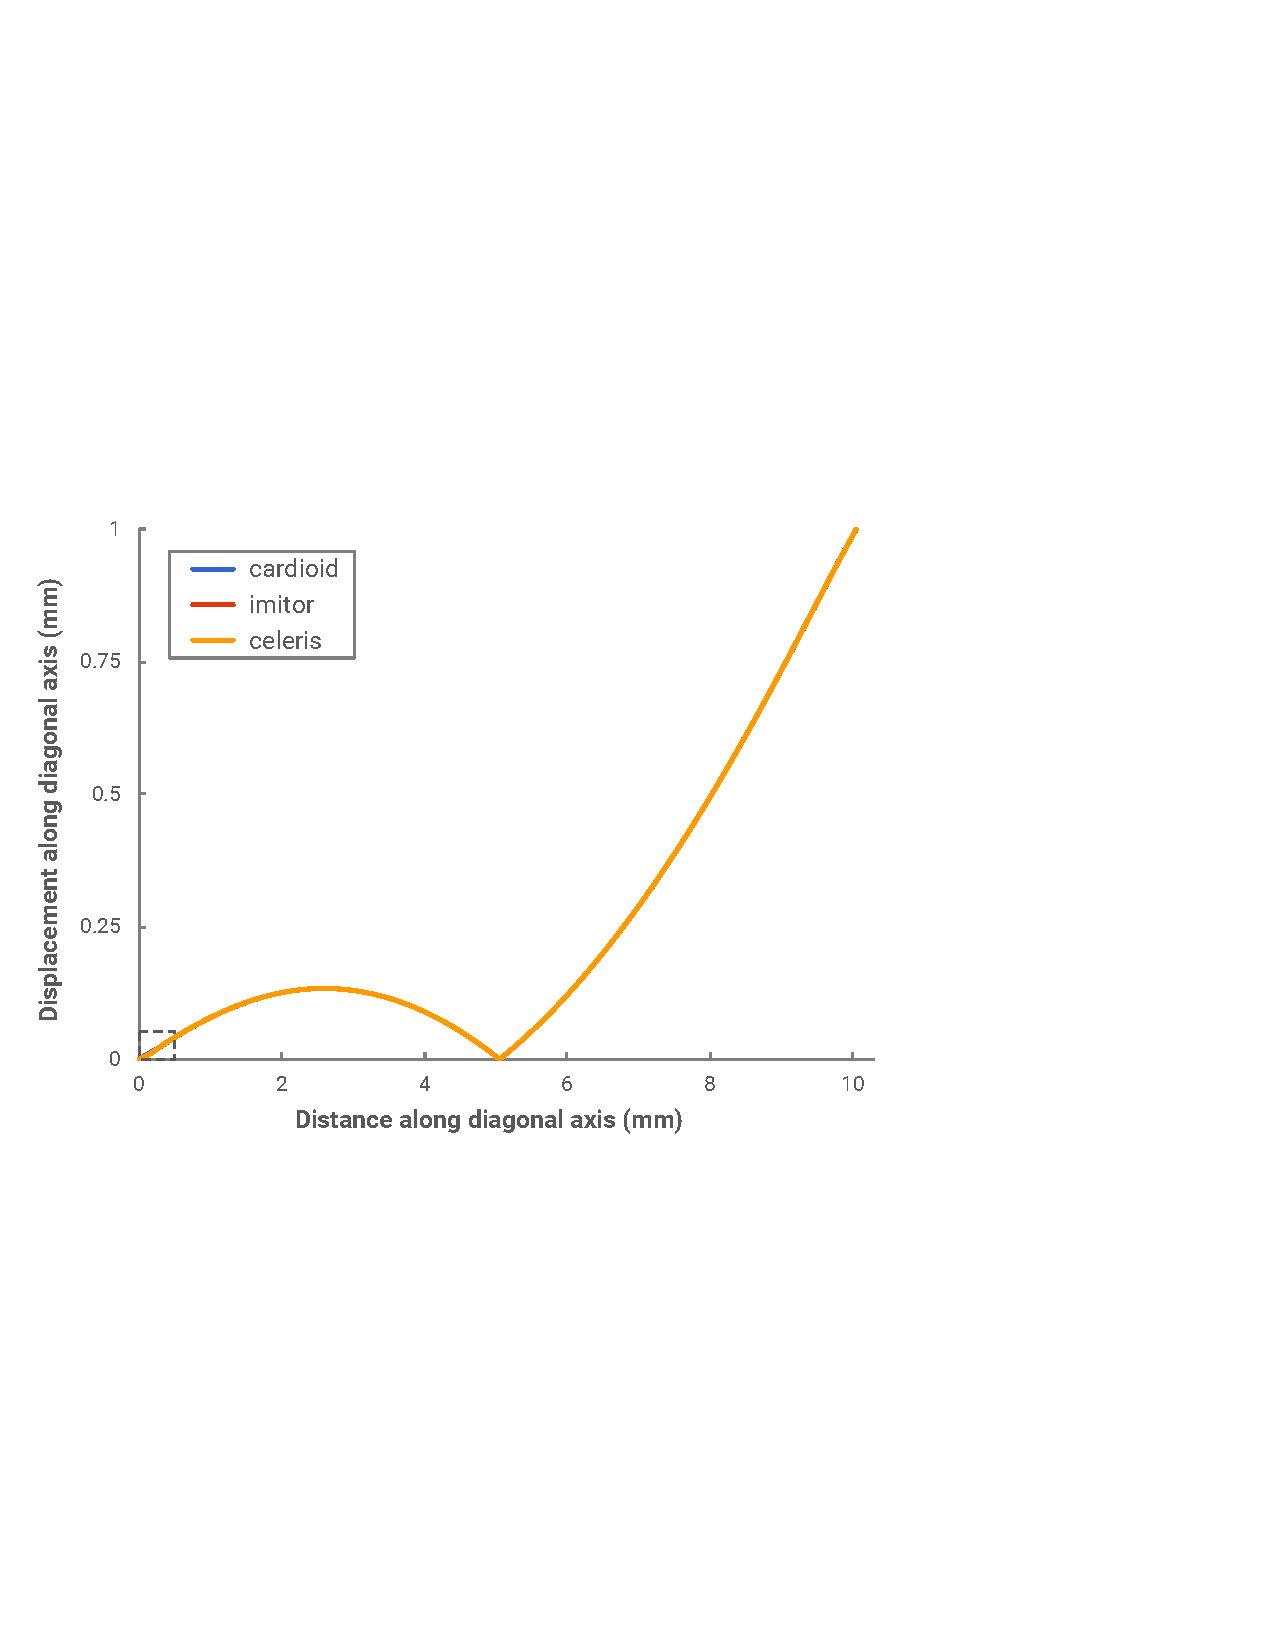
\includegraphics[scale=0.5]{media/5-verif/2-gurev3/gurev3-1.pdf}
\label{fig:gurev3-1}}		
\subfigure[]{%
		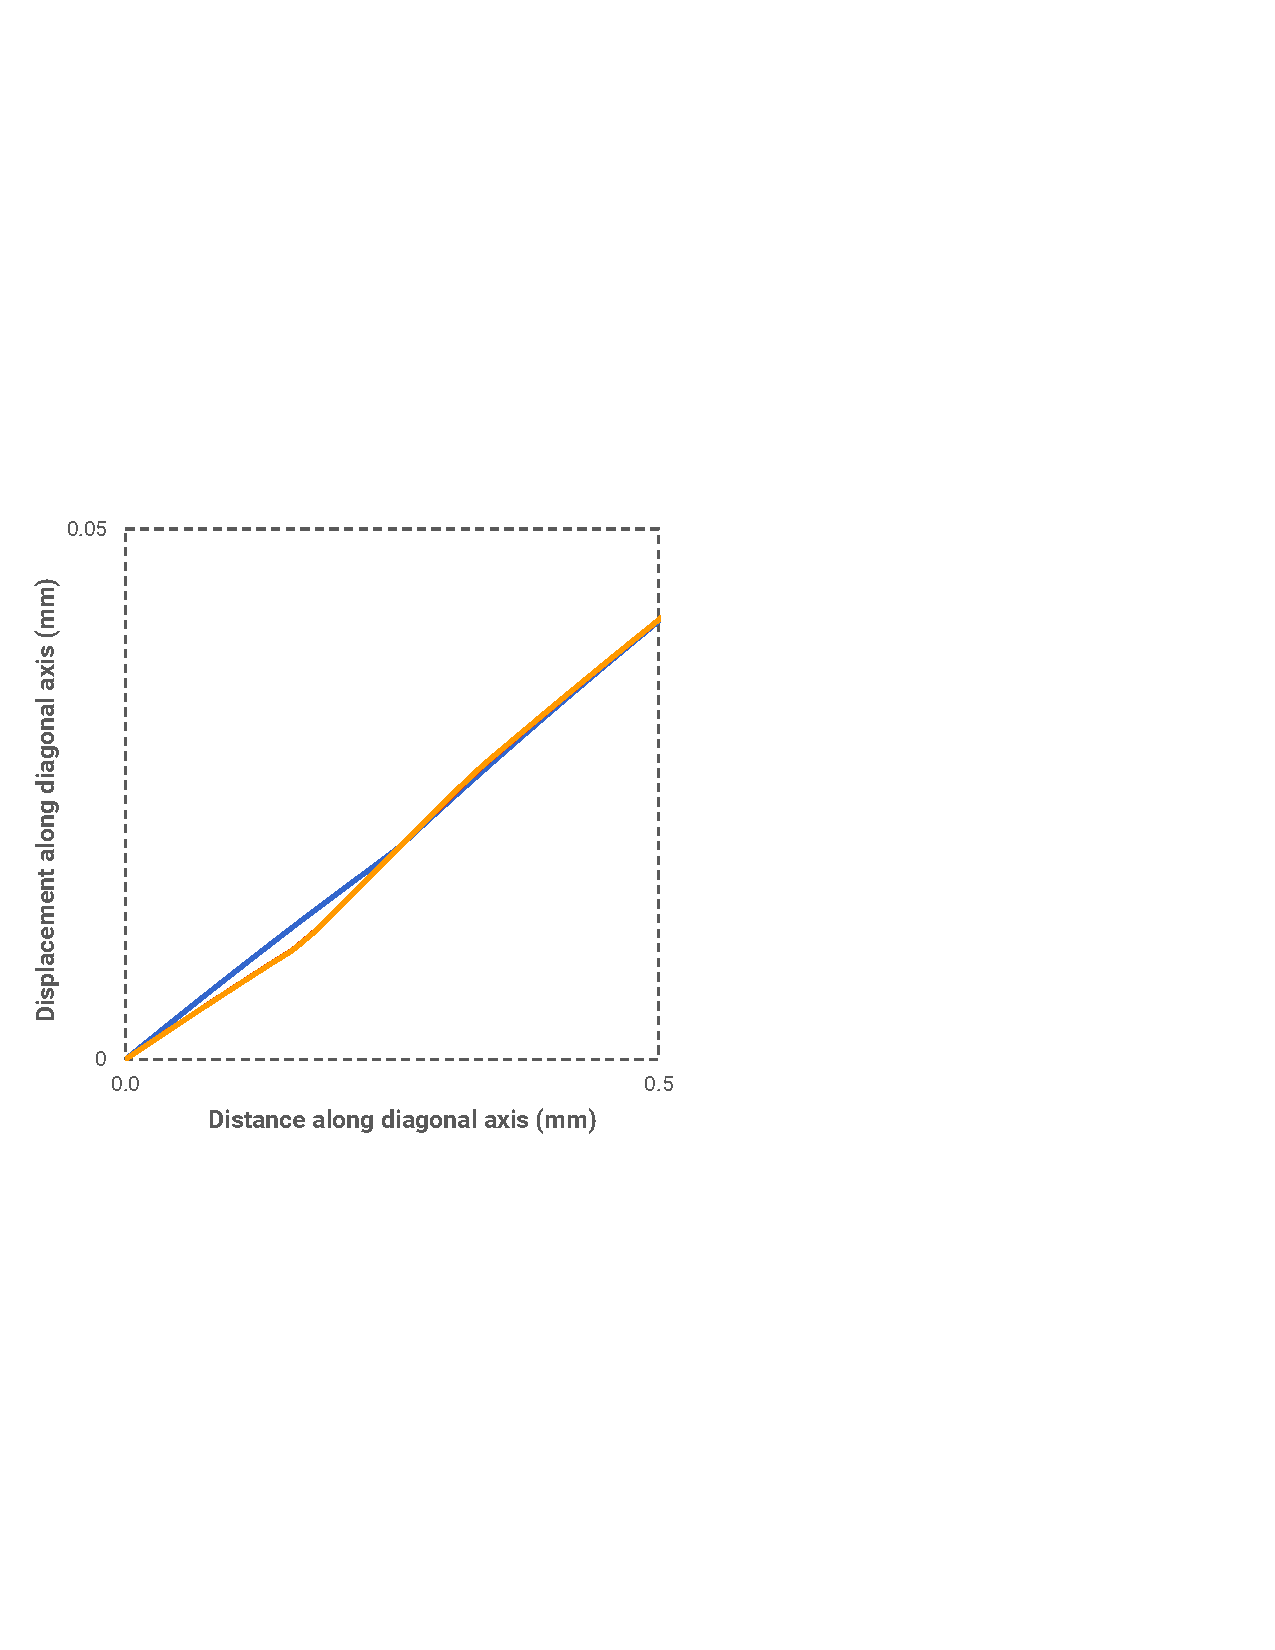
\includegraphics[scale=0.5]{media/5-verif/2-gurev3/gurev3-2.pdf}
\label{fig:gure3-2}}		
%
\caption{Results for Gurev P3 verification problem: (a) Displacement magnitude along diagonal axis, with (b) details for the fixed end of the beam. The results for imitor and Celeris are indistinguishable in these plots.}
\label{fig:gurev3}
\end{figure}

\begin{figure}[ht!]
\centering
\subfigure[]{%
		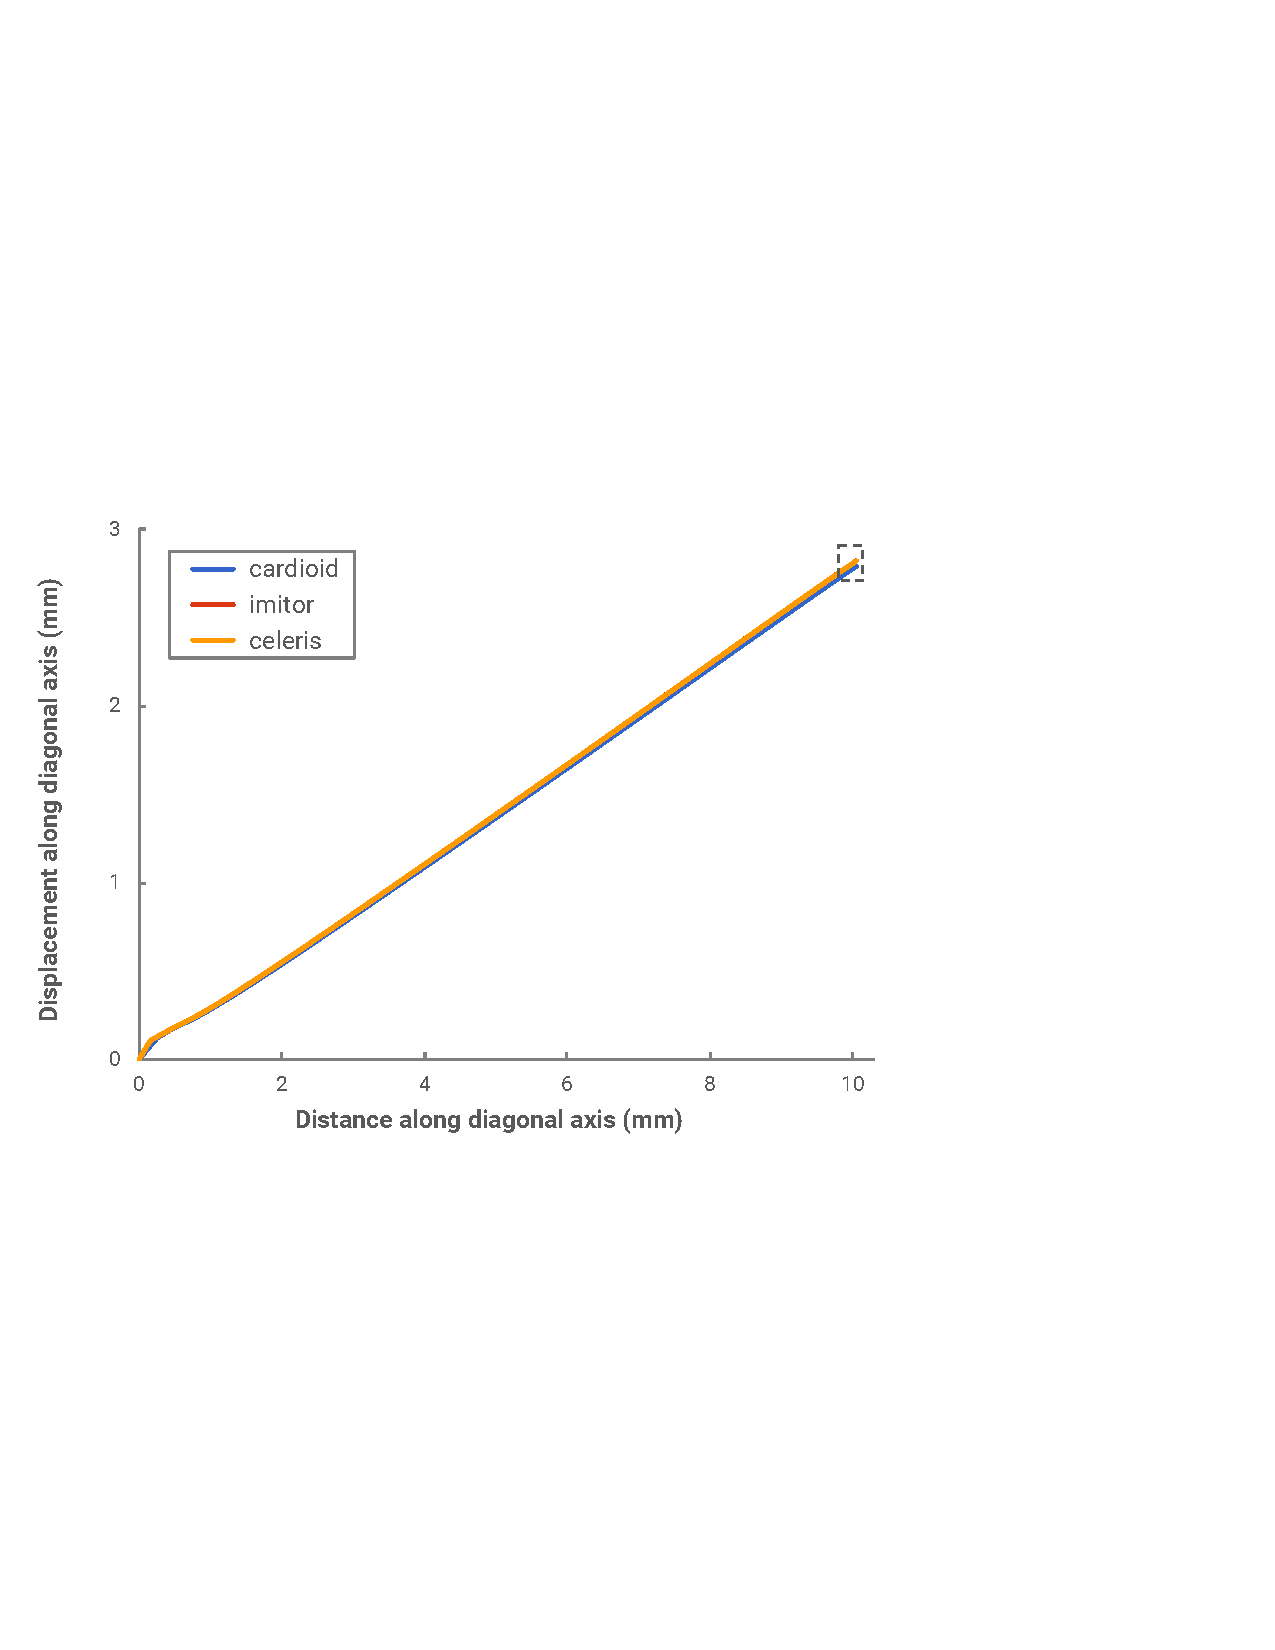
\includegraphics[scale=0.5]{media/5-verif/3-gurev4/gurev4-1.pdf}
\label{fig:gurev4-1}}		
\subfigure[]{%
		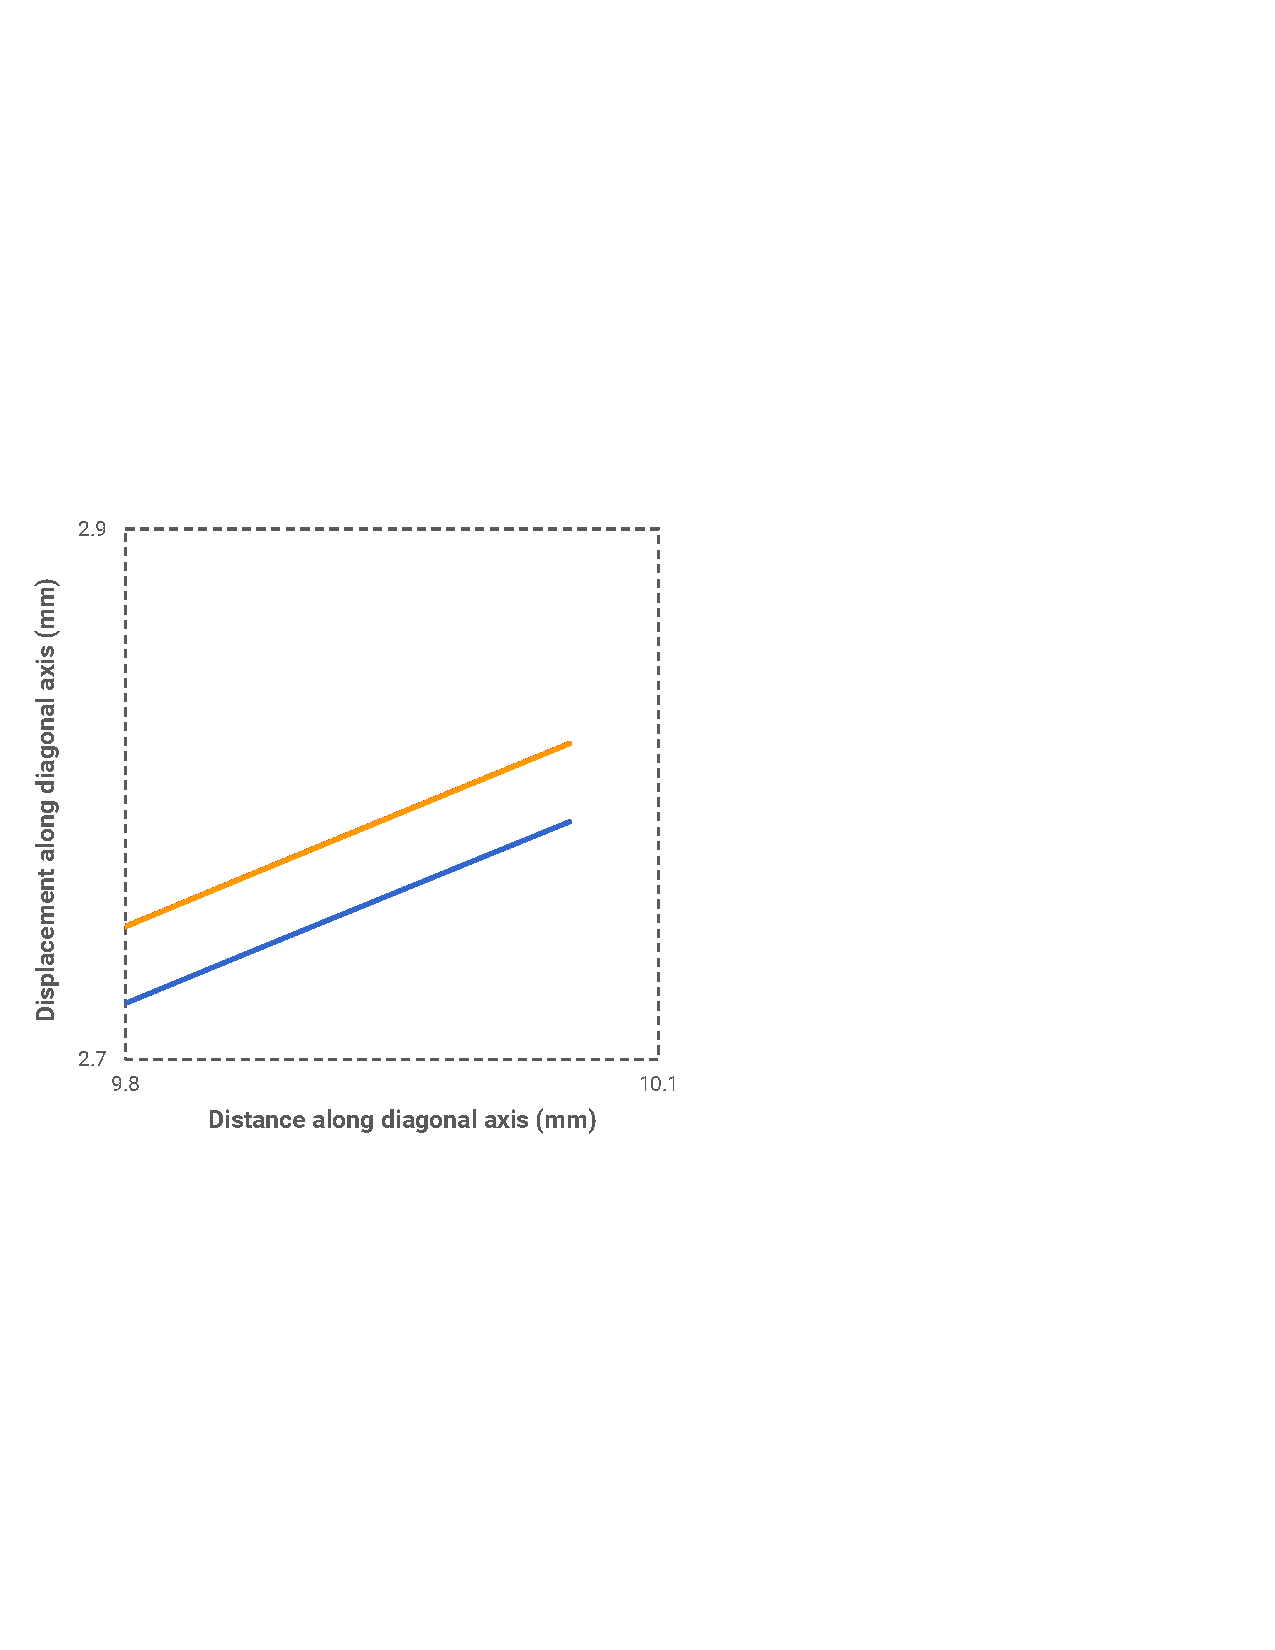
\includegraphics[scale=0.5]{media/5-verif/3-gurev4/gurev4-2.pdf}
\label{fig:gurev4-2}}		
%
\caption{Results for Gurev P4 verification problem: (a) Displacement magnitude along diagonal axis, with (b) details for the free end of the beam. The results for imitor and Celeris are indistinguishable in these plots.}
\label{fig:gurev4}
\end{figure}

\begin{figure}[ht!]
\centering
\subfigure[]{%
		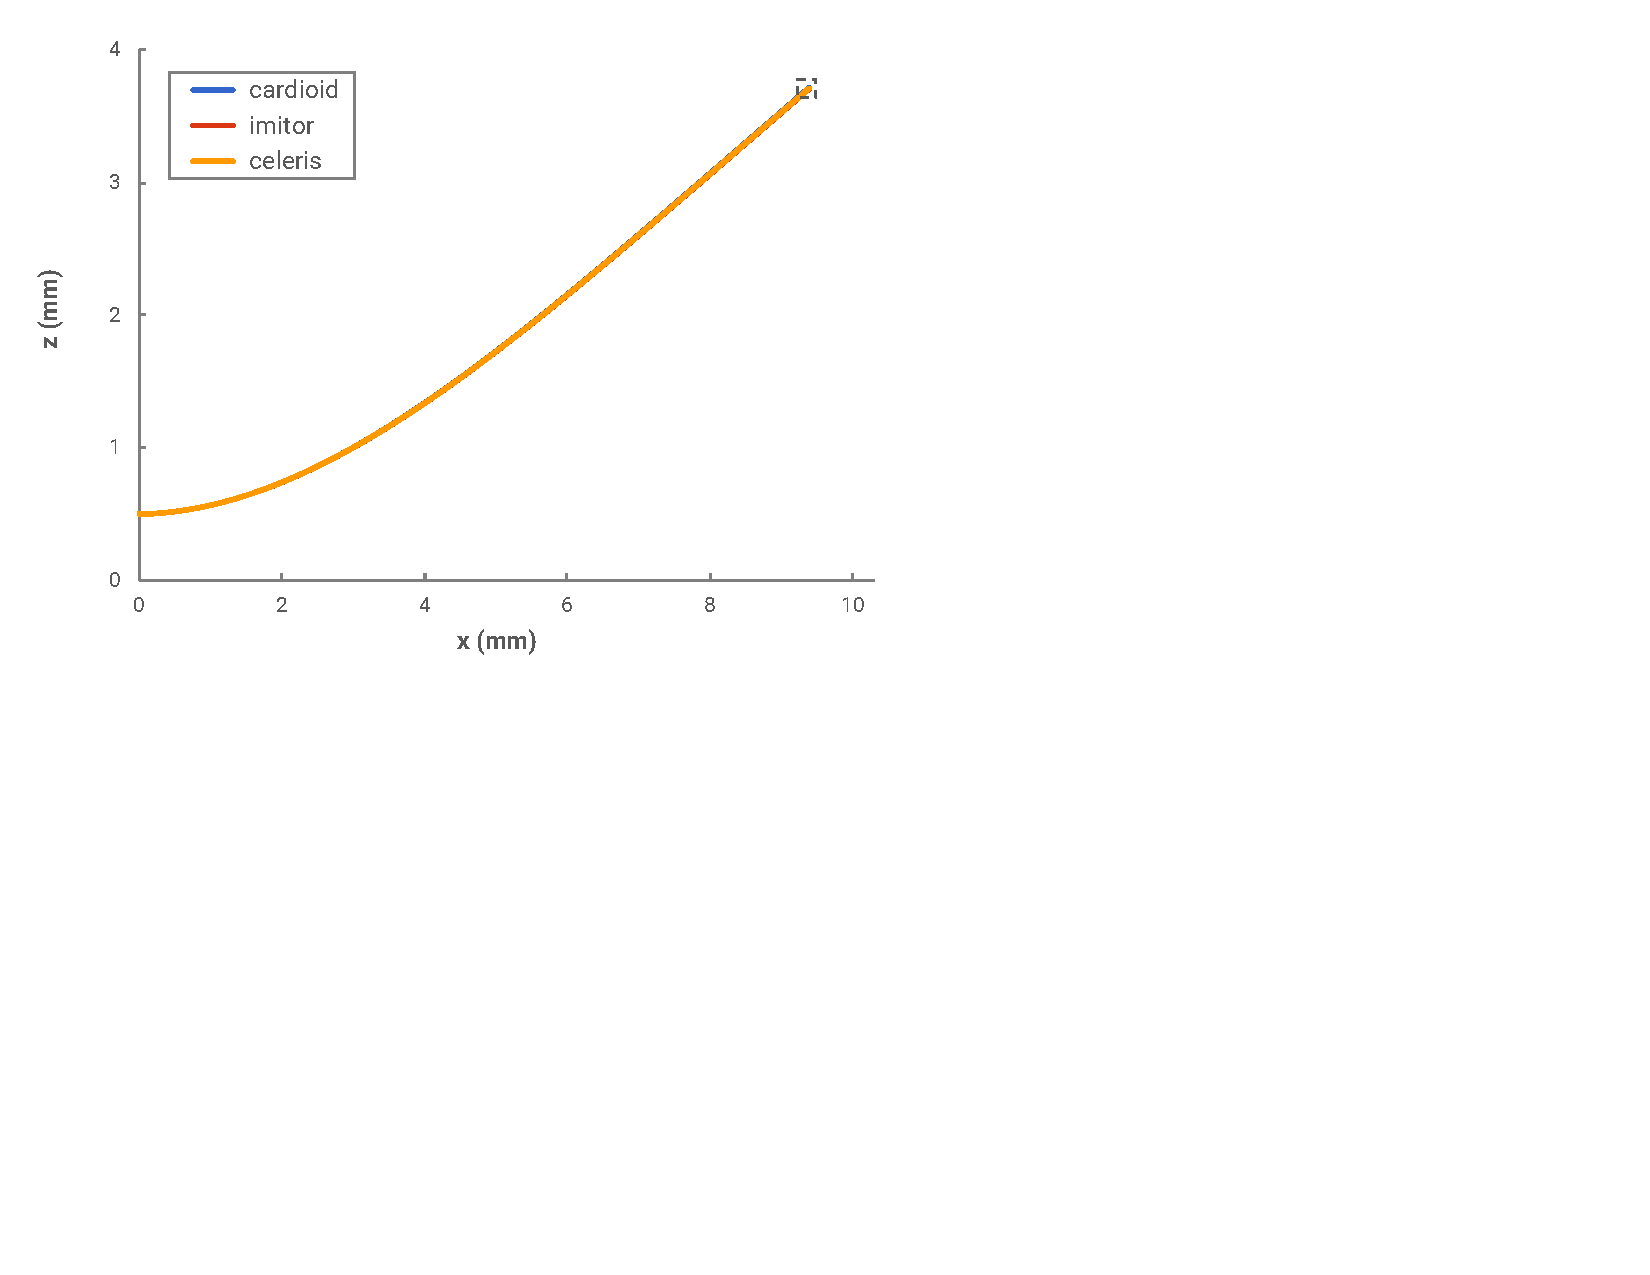
\includegraphics[scale=0.5]{media/5-verif/4-land1/land1-1.pdf}
\label{fig:land1-1}}		
\subfigure[]{%
		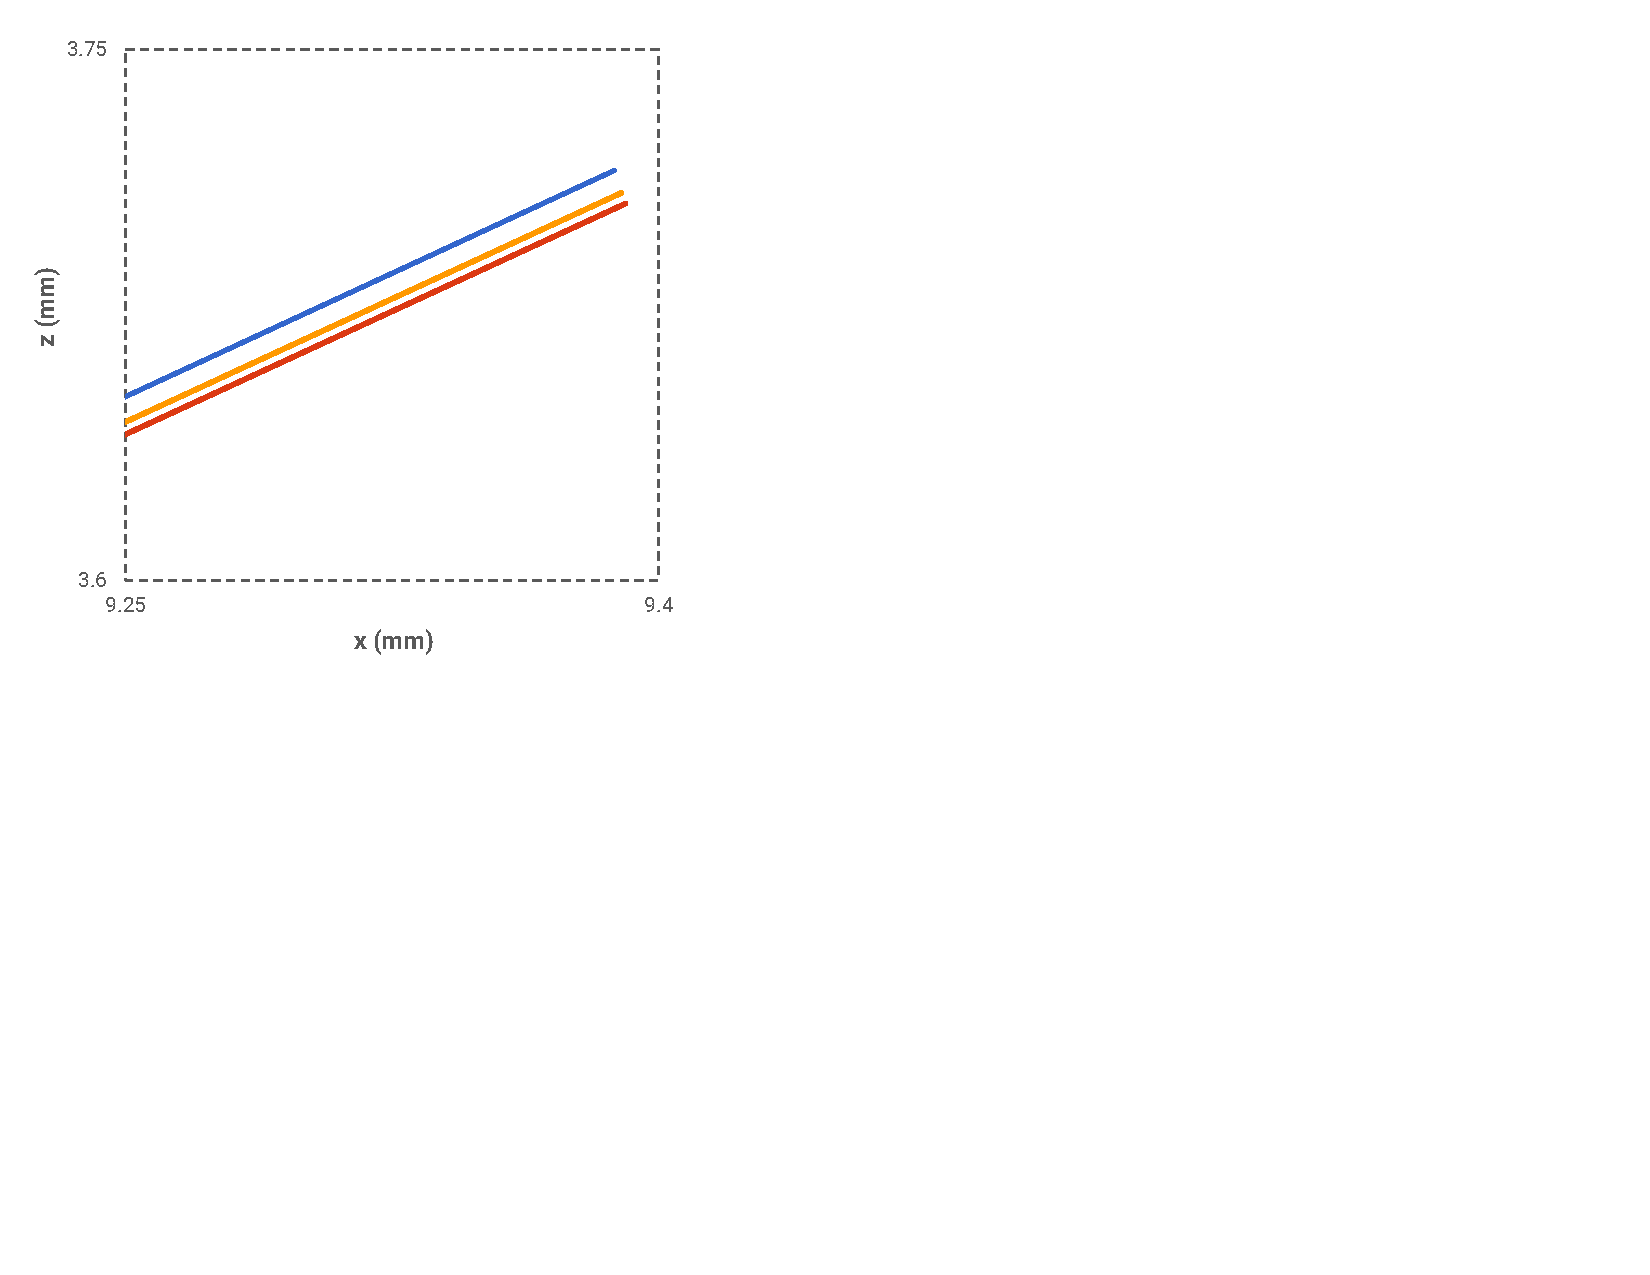
\includegraphics[scale=0.5]{media/5-verif/4-land1/land1-2.pdf}
\label{fig:land1-2}}	
\subfigure[]{%
		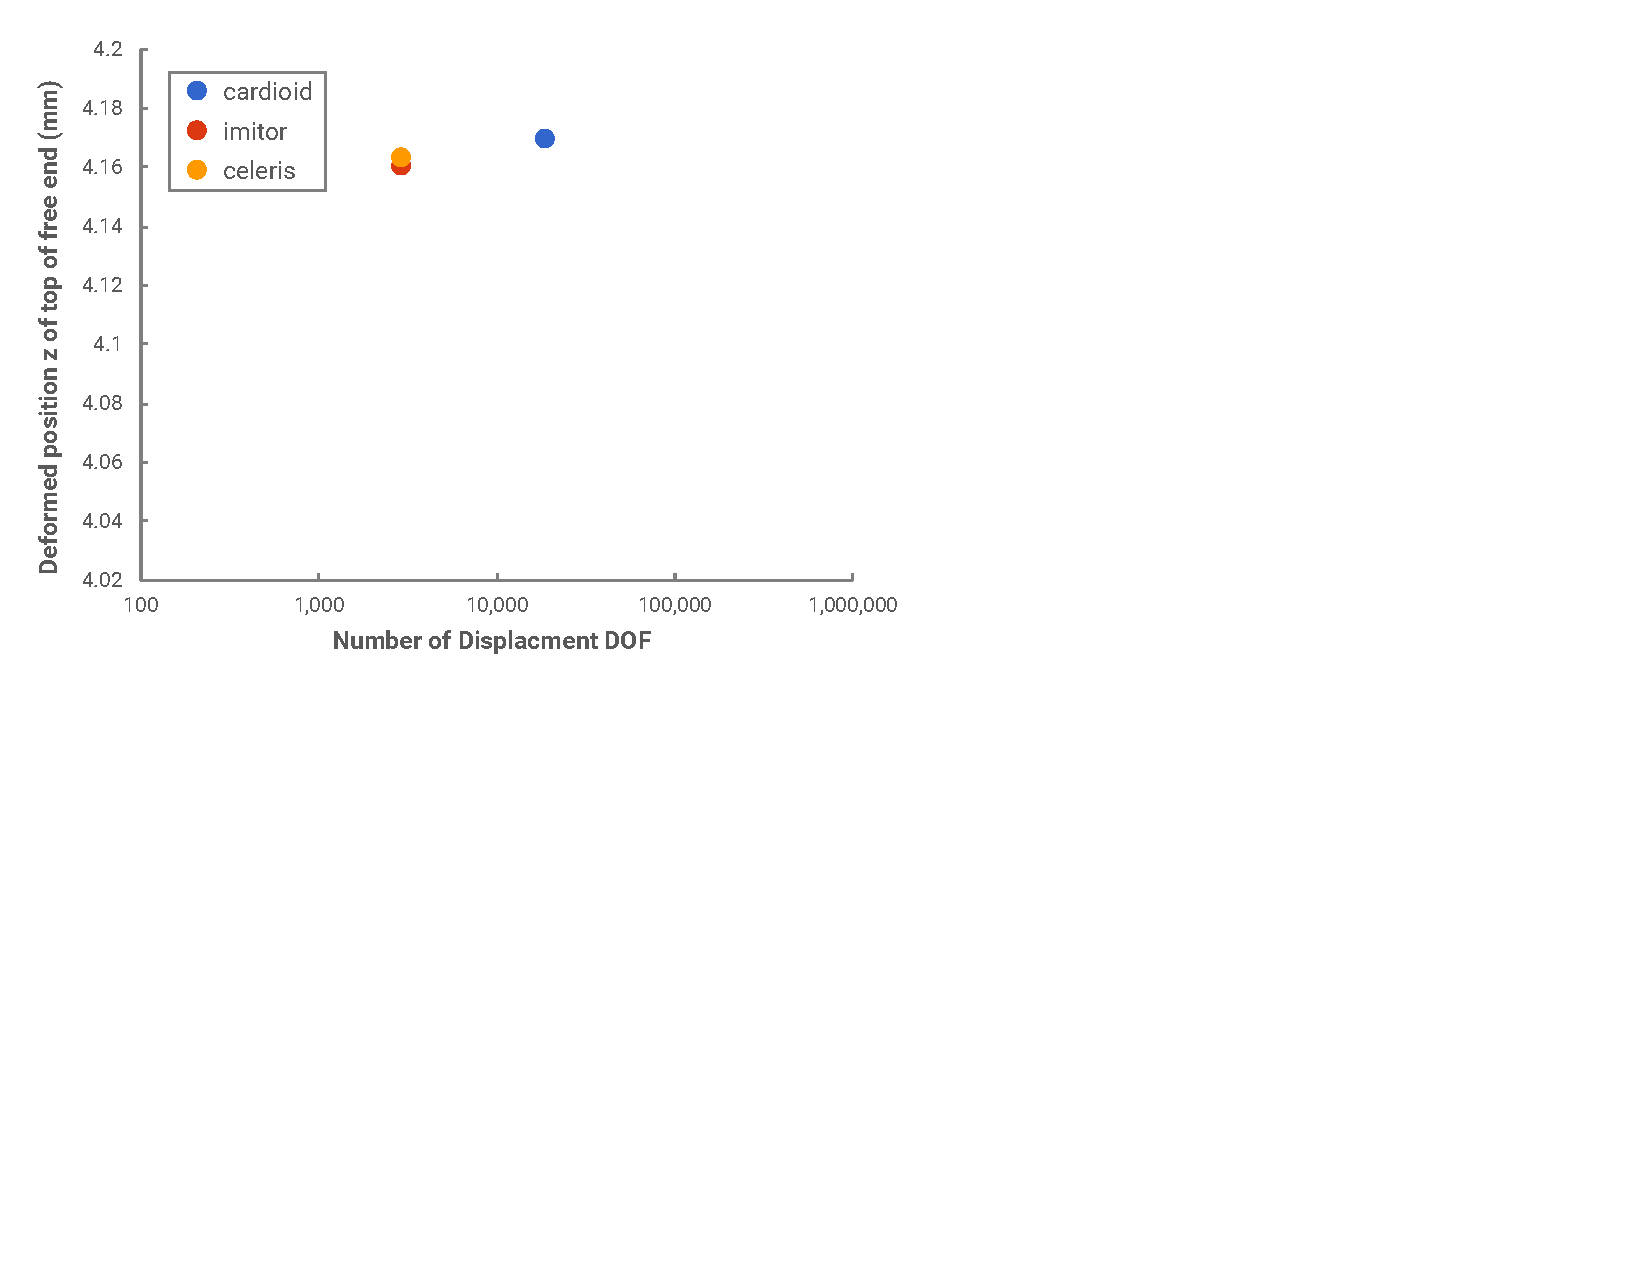
\includegraphics[scale=0.5]{media/5-verif/4-land1/land1-3.pdf}
\label{fig:land1-3}}			
%
\caption{Results for Land P1 verification problem: (a) Deformed position of midline, with (b) details for the free end of the beam. Panel (c) shows the deformed position of the point $\mathbf{X} = (10, 0.5, 1)$ for each of the simulation codes.}
\label{fig:land1}
\end{figure}


\begin{figure}[ht!]
\centering
\subfigure[]{%
		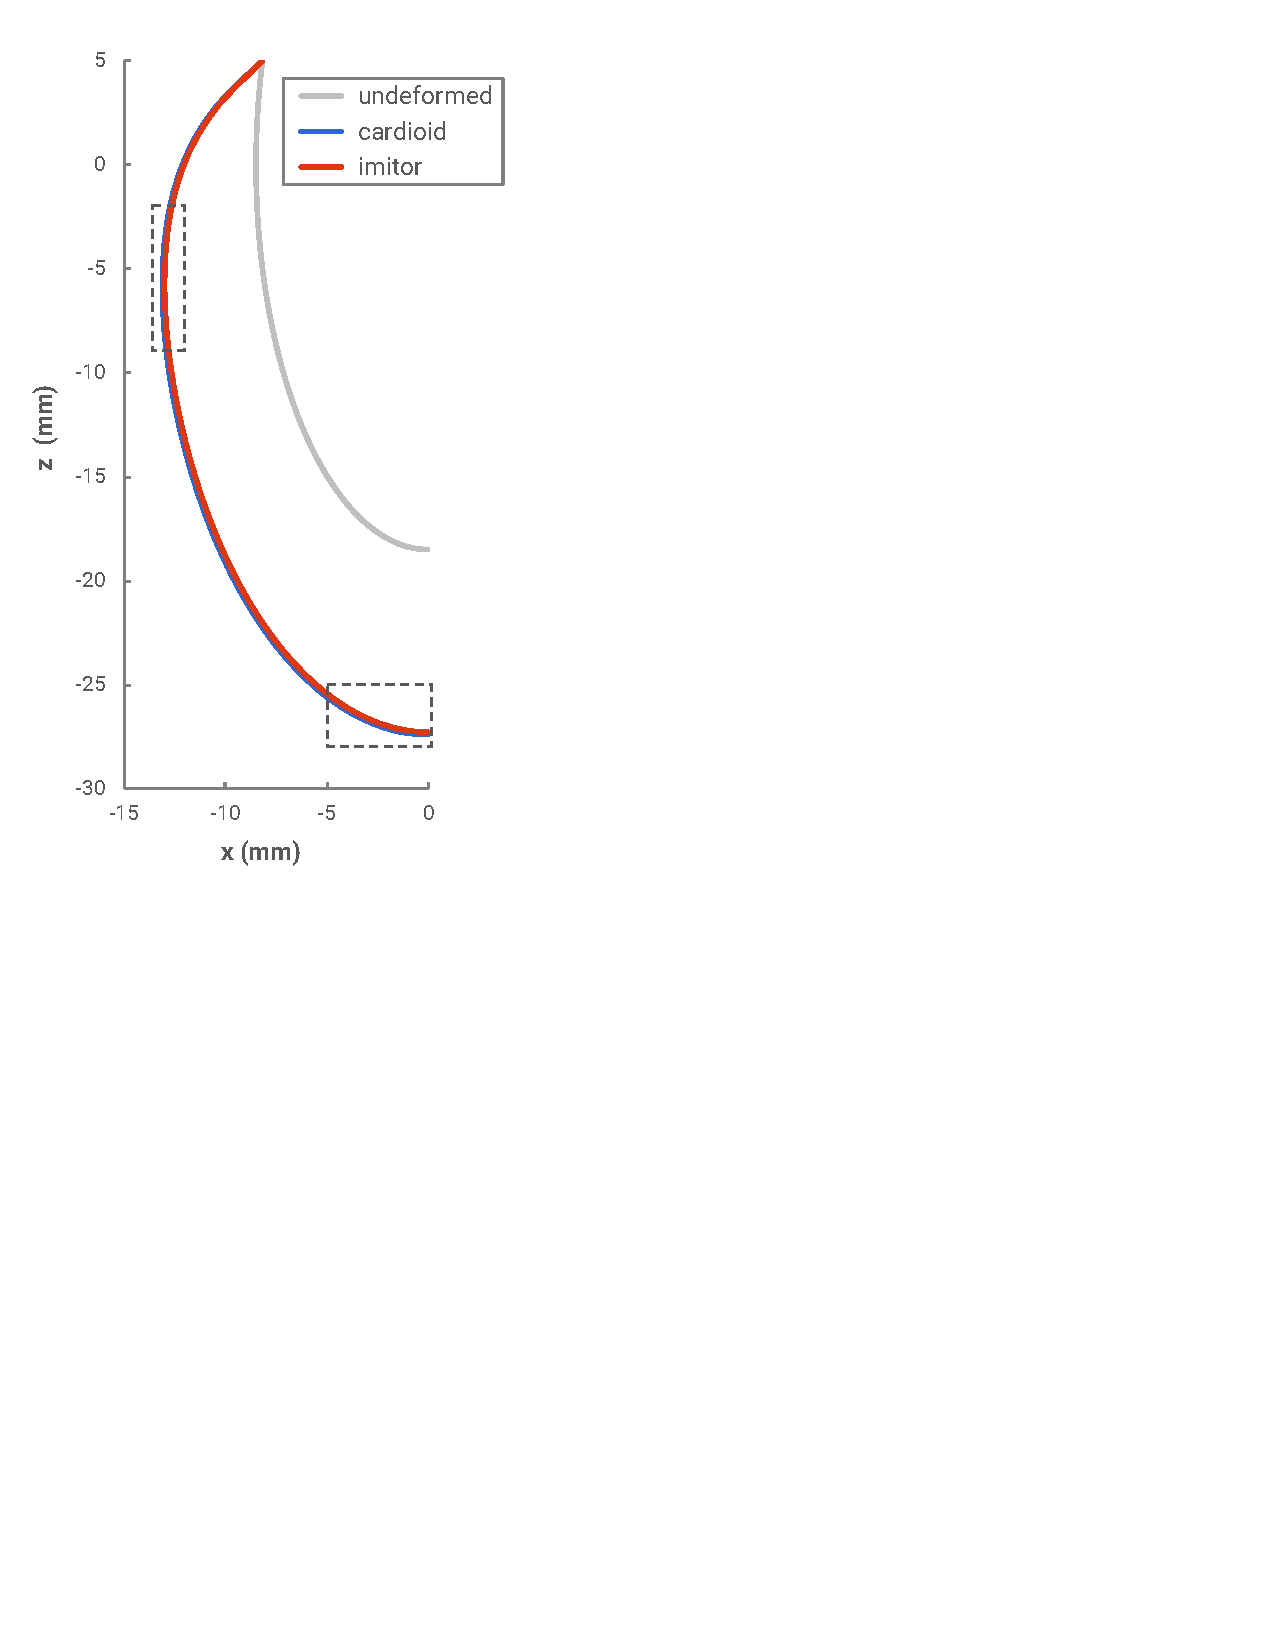
\includegraphics[scale=0.5]{media/5-verif/5-land2/land2-1.pdf}
\label{fig:land2-1}}		
\subfigure[]{%
		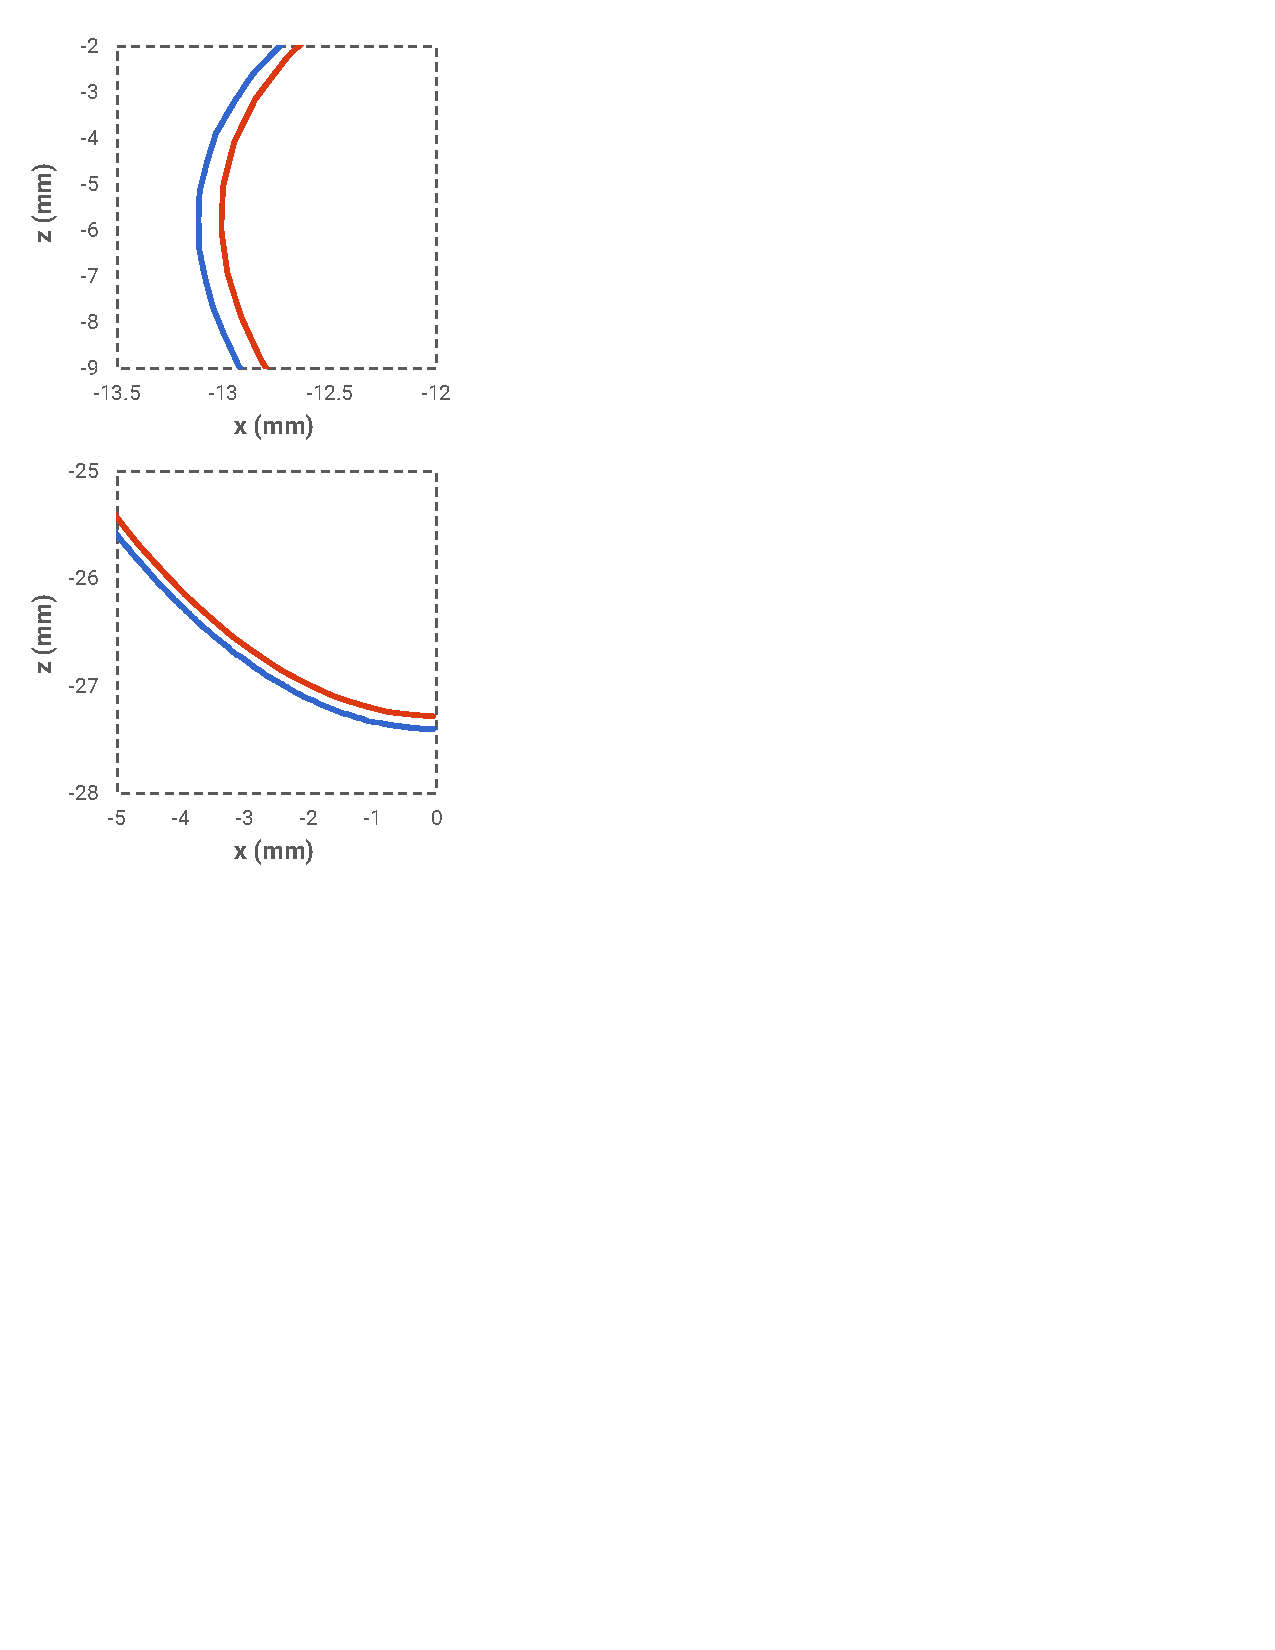
\includegraphics[scale=0.5]{media/5-verif/5-land2/land2-2.pdf}
\label{fig:land2-2}}	
\subfigure[]{%
		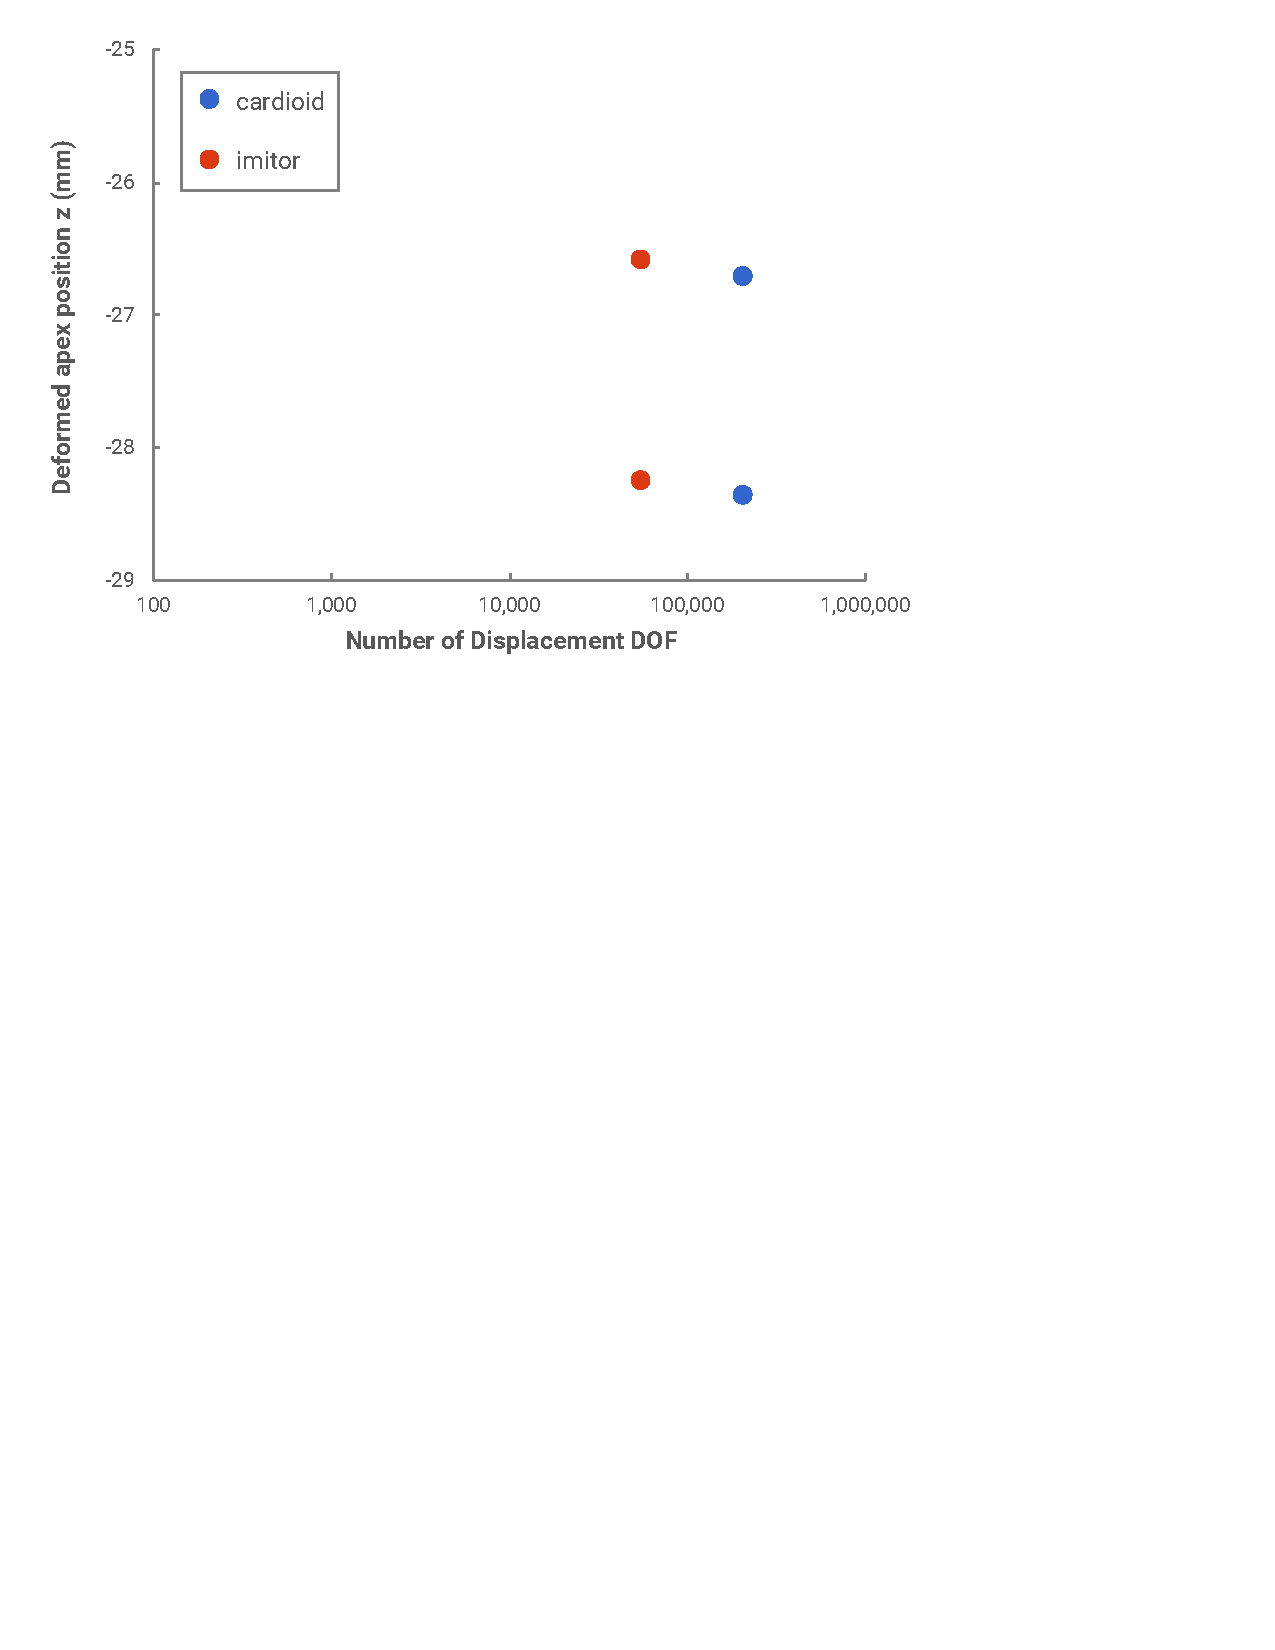
\includegraphics[scale=0.5]{media/5-verif/5-land2/land2-3.pdf}
\label{fig:land2-3}}			
%
\caption{Results for Land P2 verification problem: (a) Deformed position of middle of the ventricle wall, with (b) details at the inflection point (top right) and the apical region (bottom right). Panel (c) shows the deformed position of the apex at the endo- and epicardium for each of the simulation codes.}
\label{fig:land2}
\end{figure}

\begin{figure}[ht!]
\centering
\subfigure[]{%
		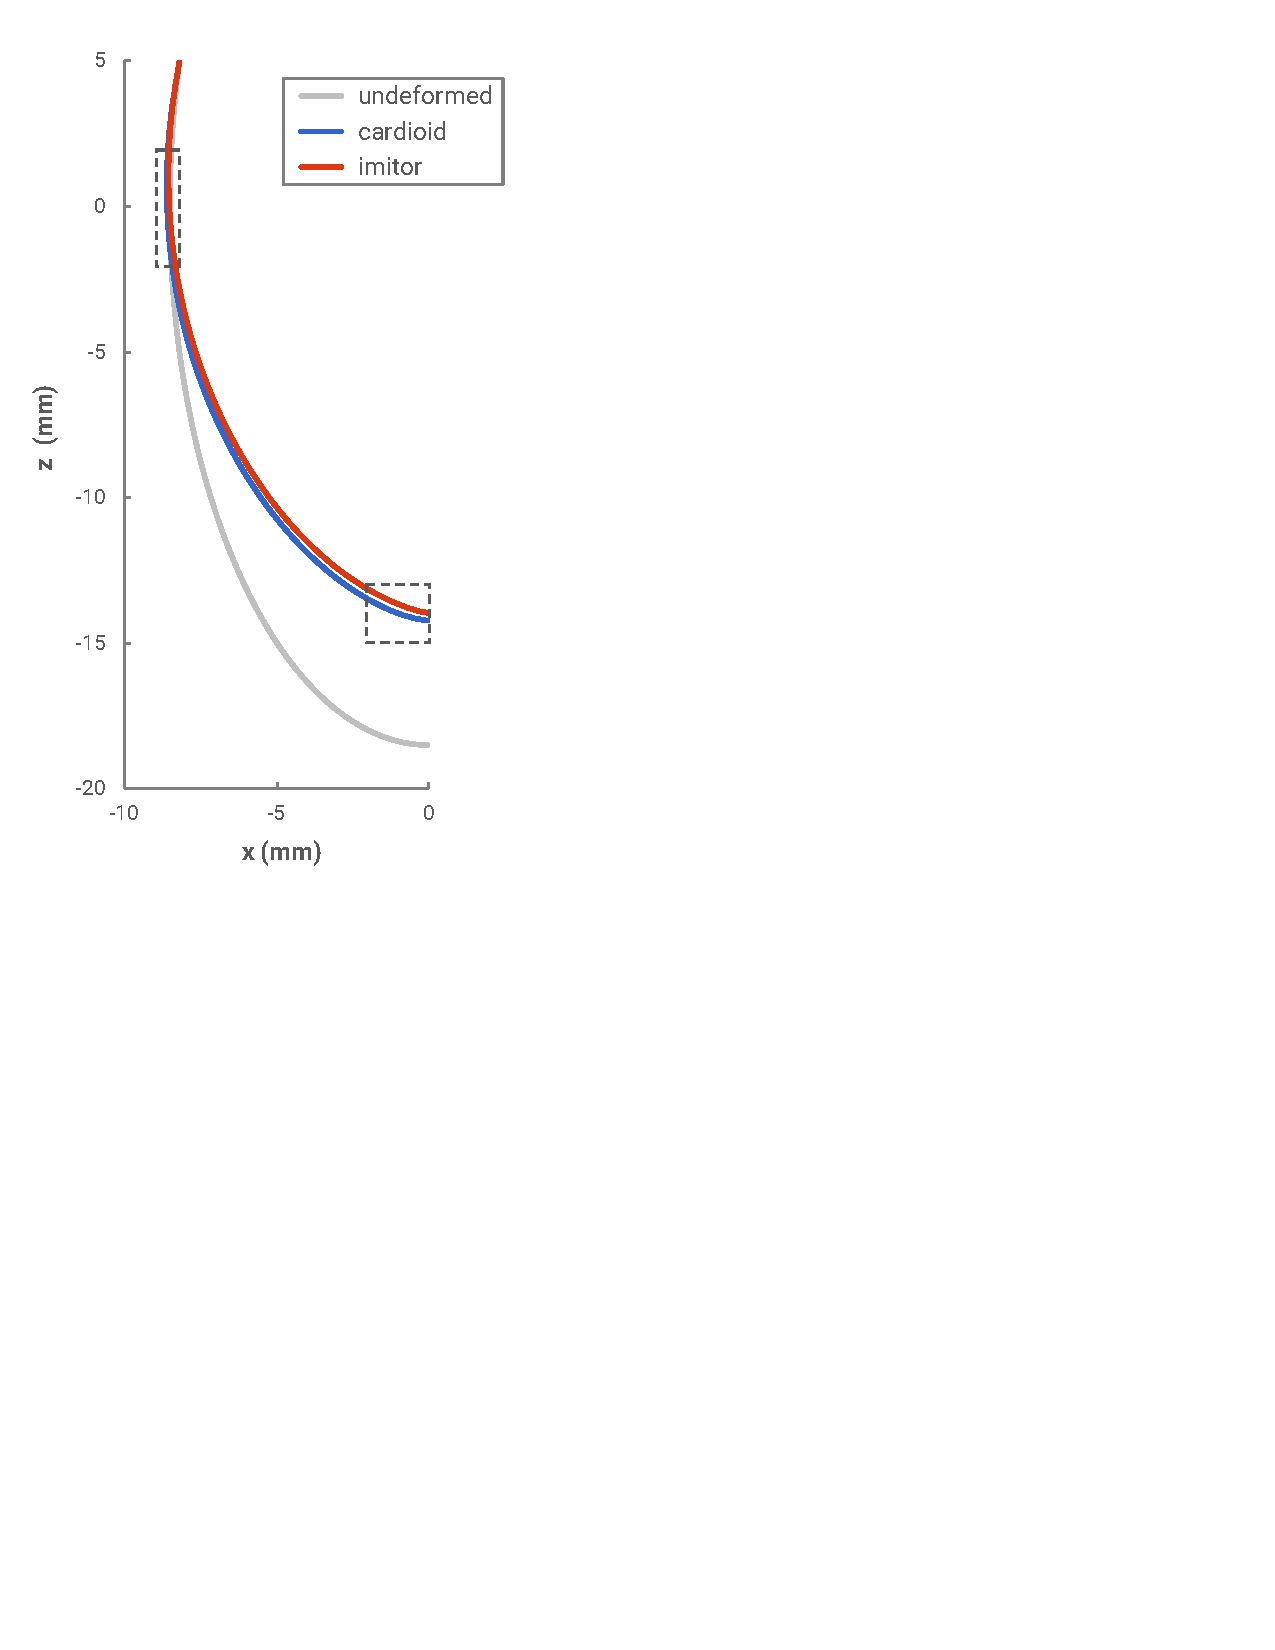
\includegraphics[scale=0.5]{media/5-verif/6-land3/land3-1.pdf}
\label{fig:land3-1}}		
\subfigure[]{%
		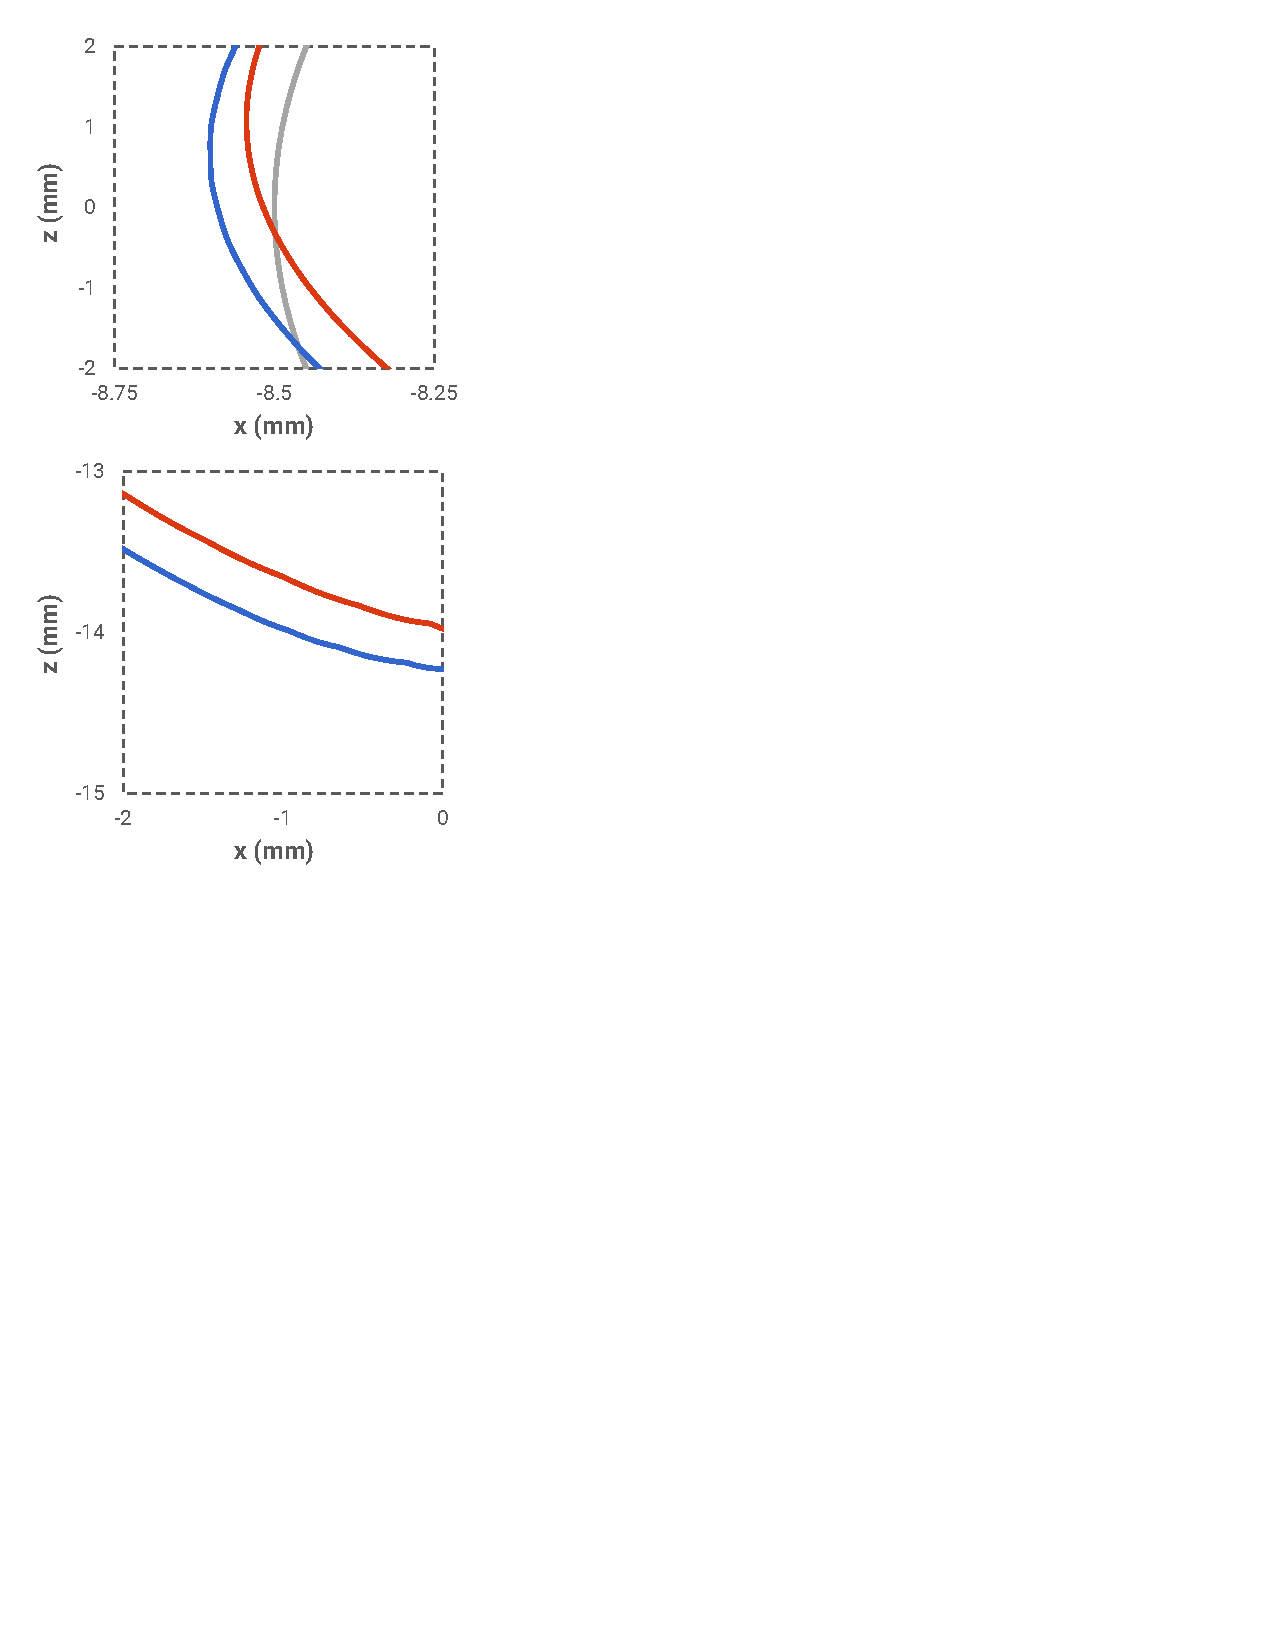
\includegraphics[scale=0.5]{media/5-verif/6-land3/land3-2.pdf}
\label{fig:land3-2}}	
%
\caption{Results for Land P3 verification problem: (a) Deformed position of middle of the ventricle wall, with (b) details at the inflection point (top right) and the apical region (bottom right).}
\label{fig:land3}
\end{figure}

\begin{figure}[ht!]
\centering
\subfigure[]{%
		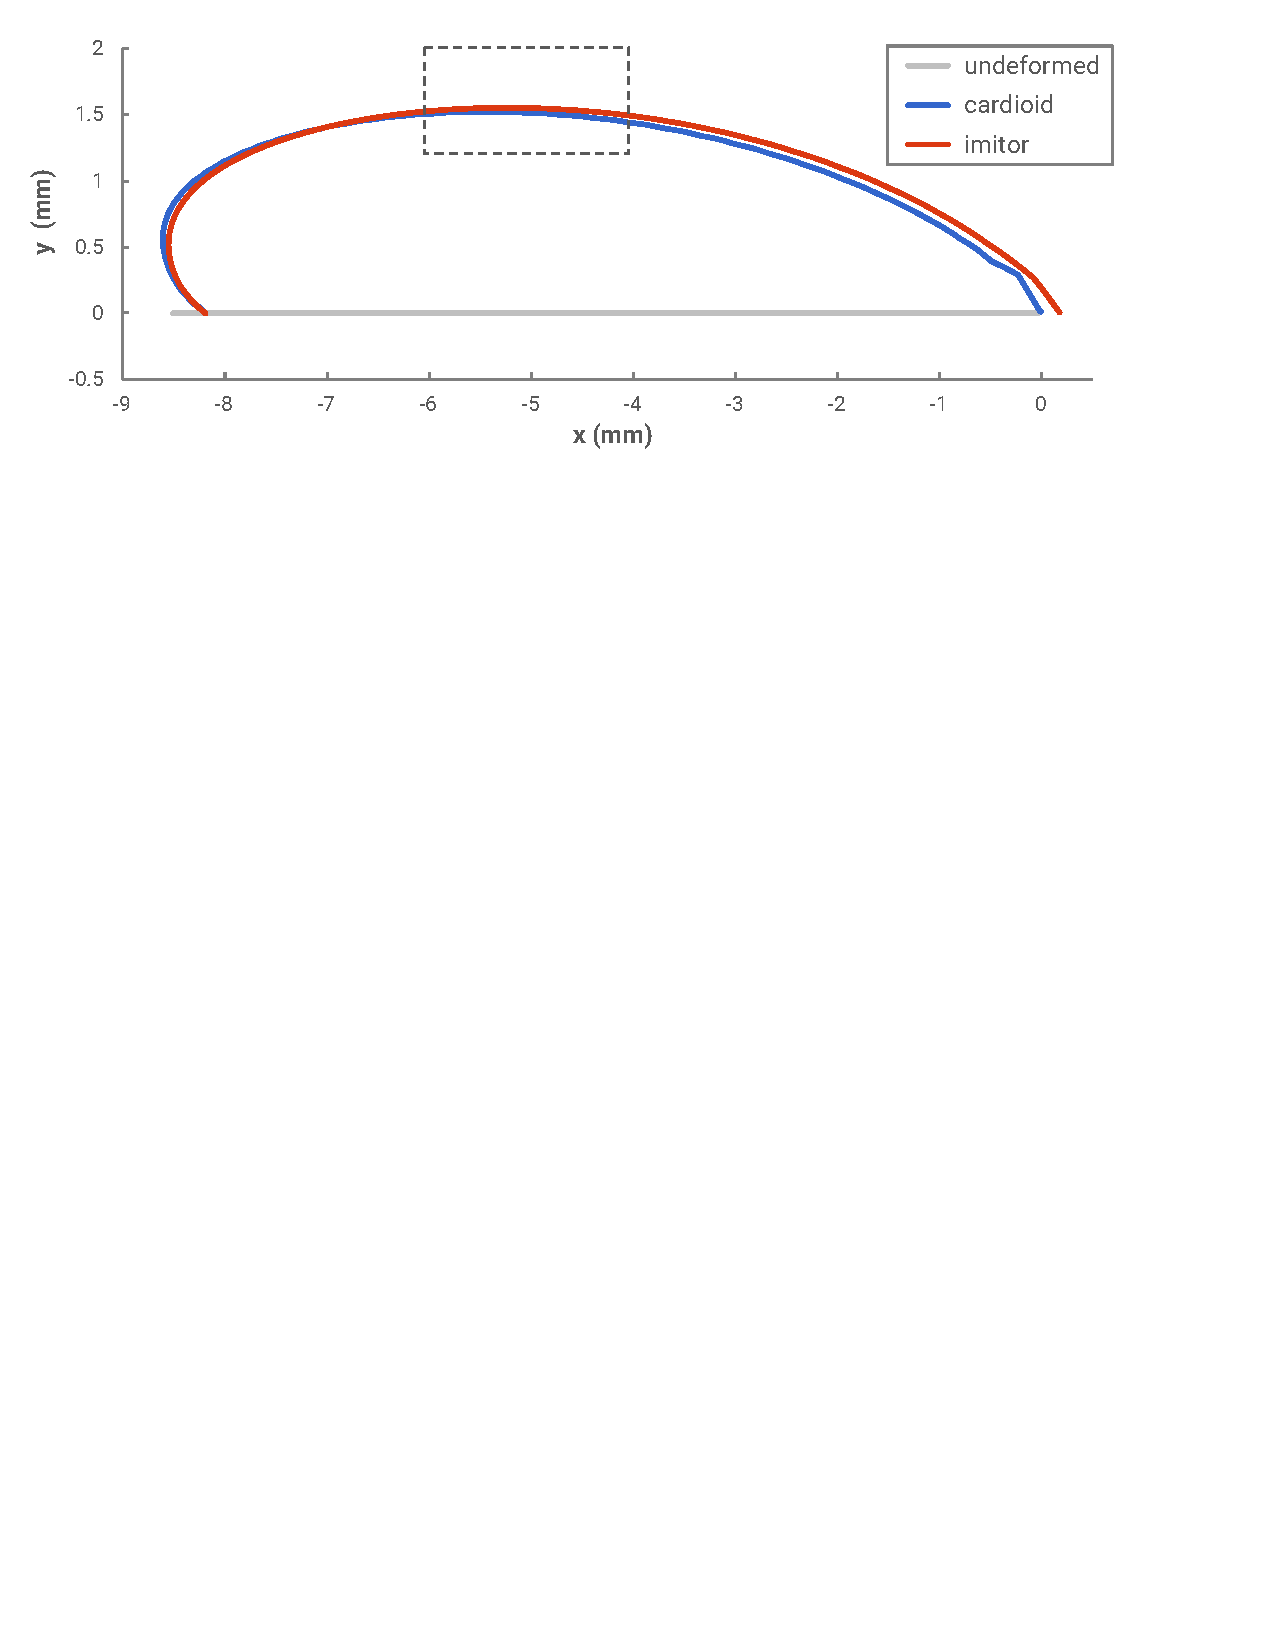
\includegraphics[scale=0.5]{media/5-verif/6-land3/land3-3.pdf}
\label{fig:land3.2-1}}		
\subfigure[]{%
		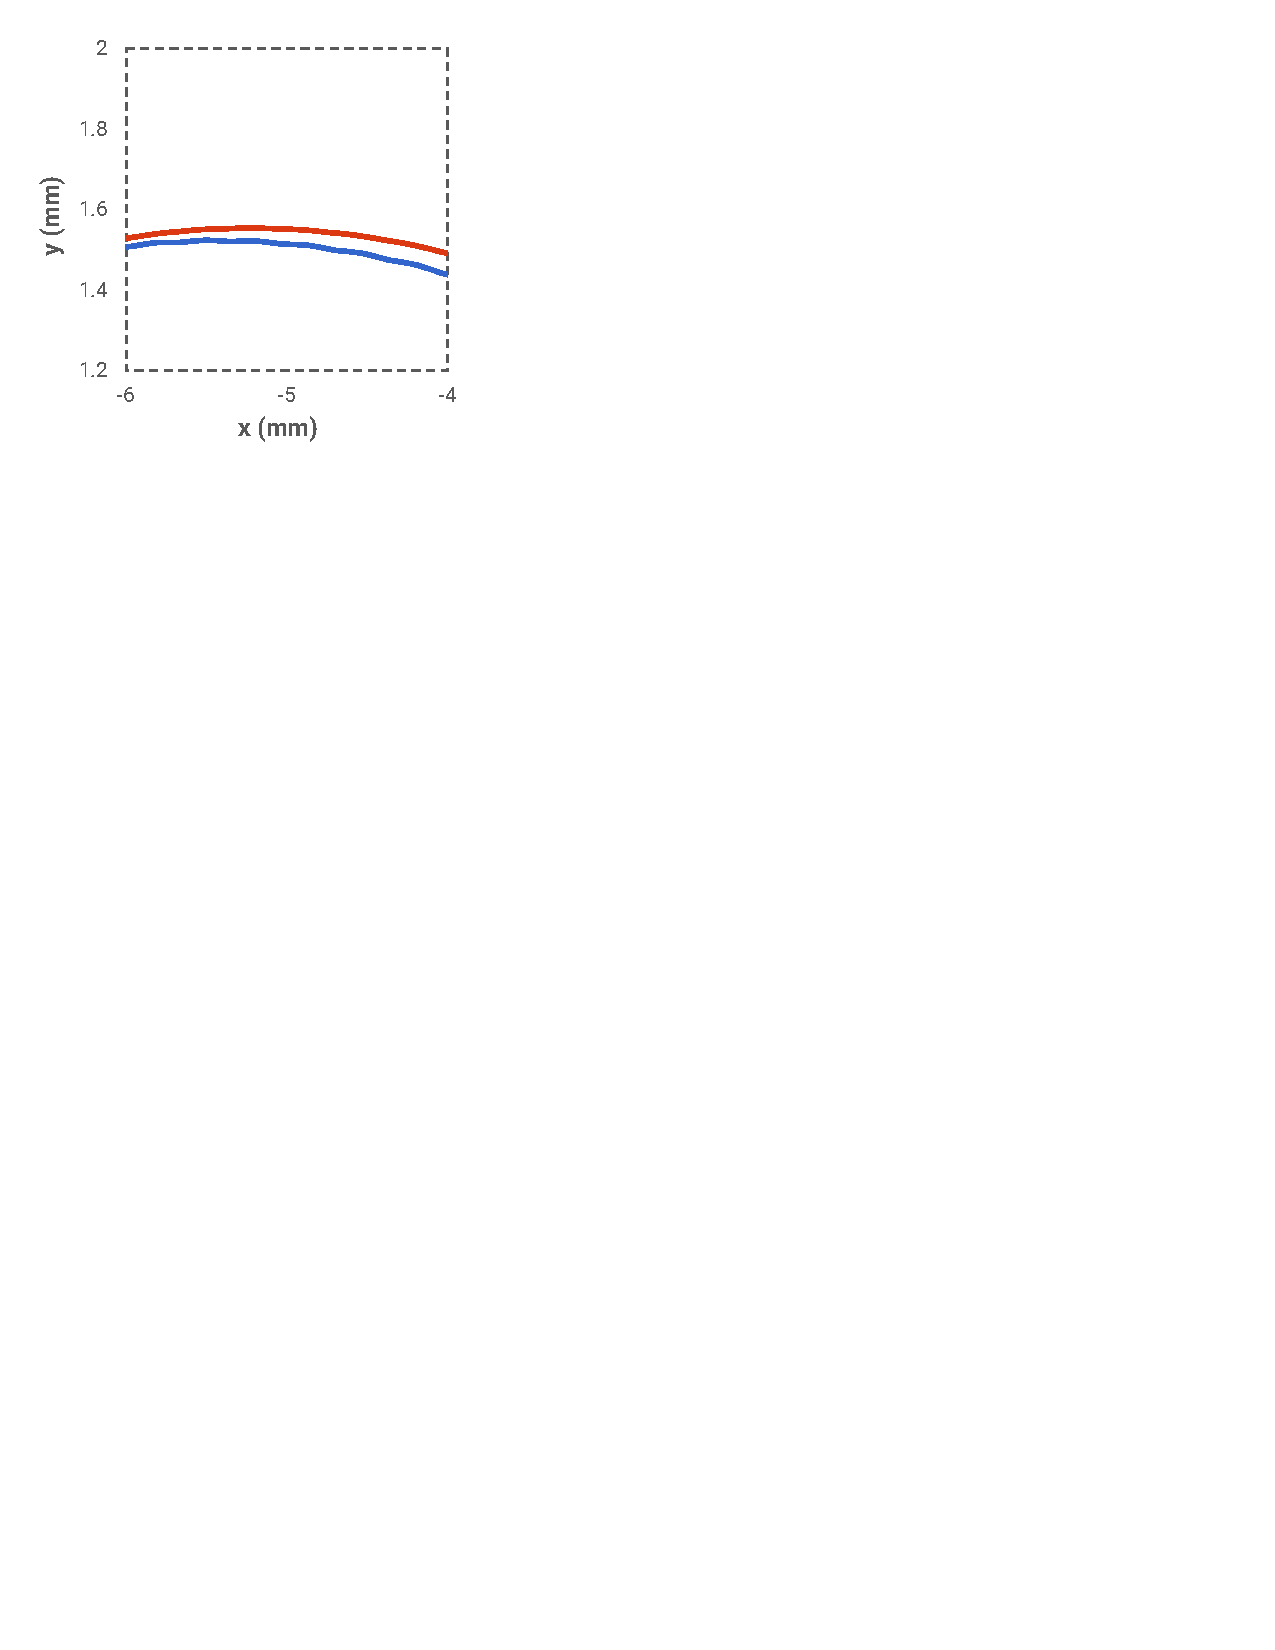
\includegraphics[scale=0.5]{media/5-verif/6-land3/land3-4.pdf}		
\label{fig:land3.2-2}}	
\subfigure[]{%
		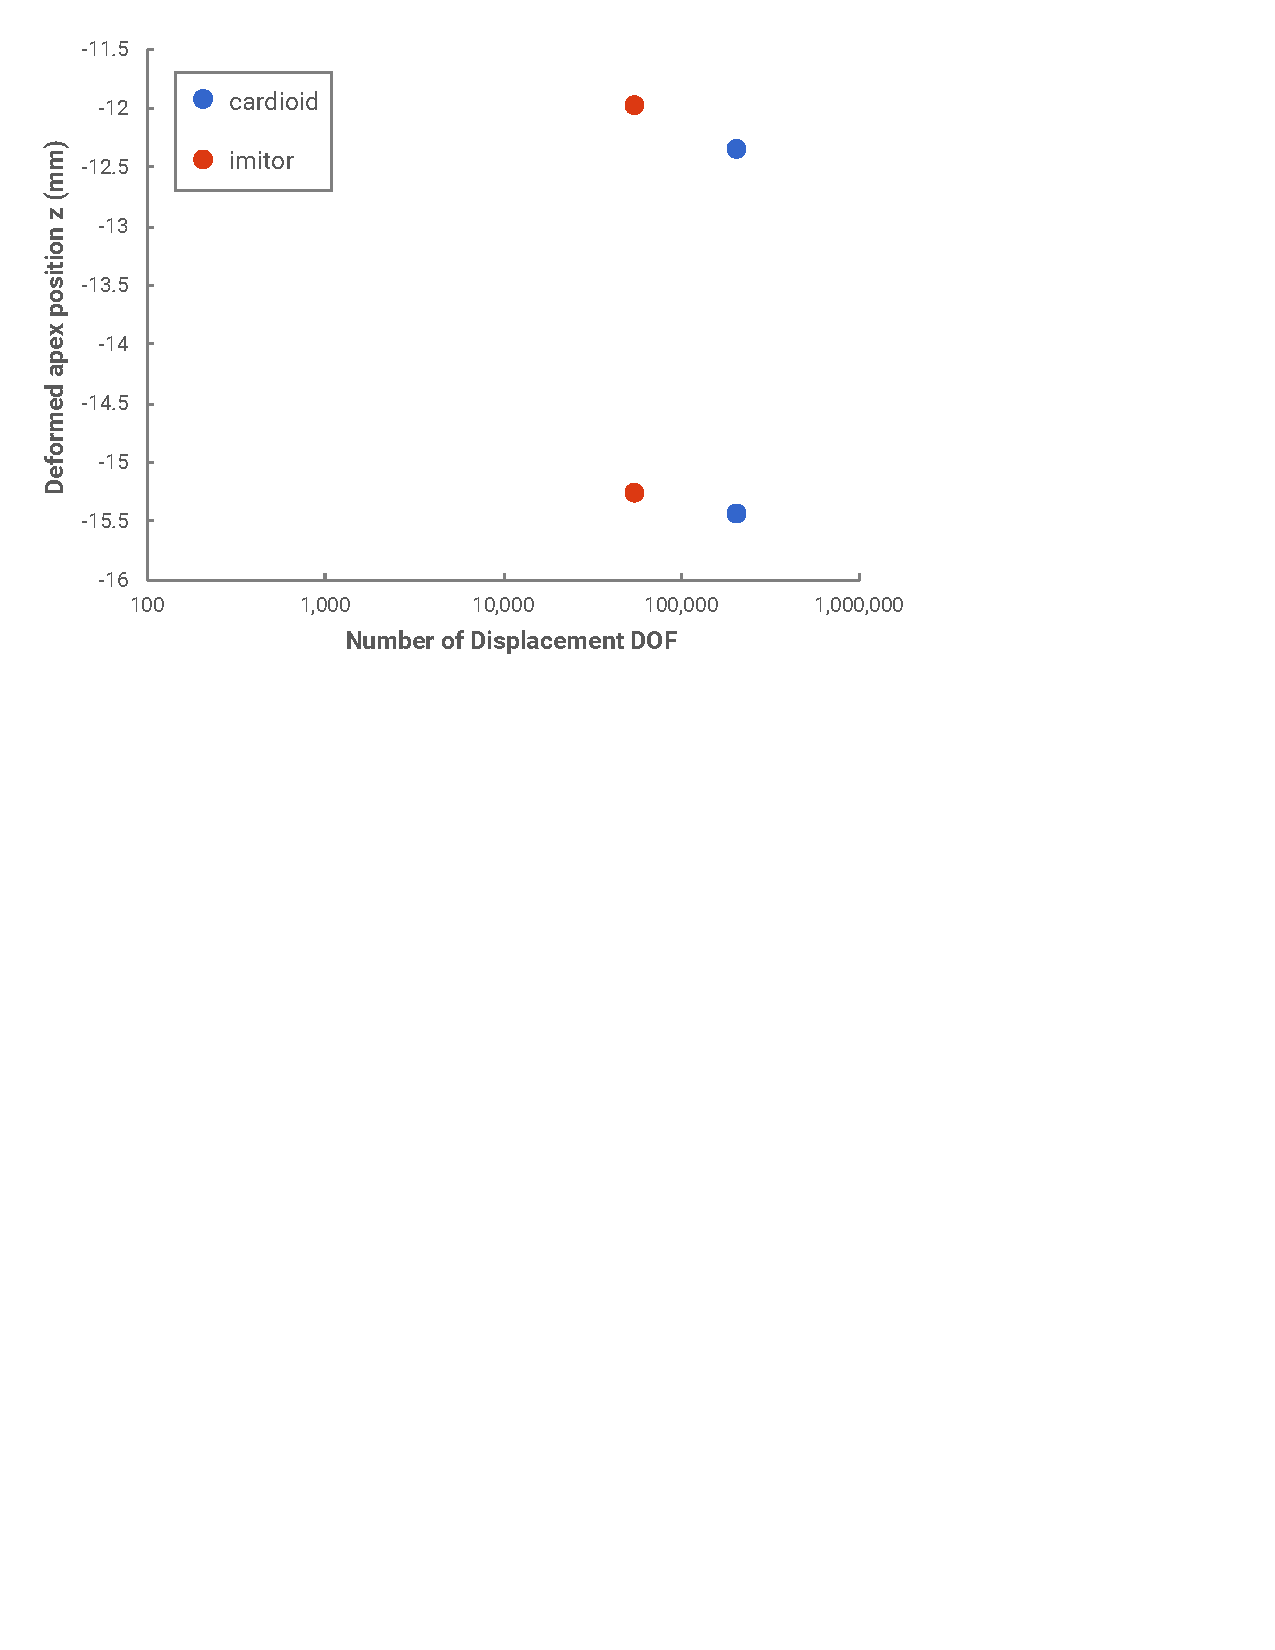
\includegraphics[scale=0.5]{media/5-verif/6-land3/land3-5.pdf}
\label{fig:land3.2-3}}			
	
%
\caption{Results for Land P3 verification problem: (a) The same deformed position of middle of the ventricle wall, shown in the $x-y$ plane, with (b) details at the inflection point. Panel (c) shows the deformed position of the apex at the endo- and epicardium for each of the simulation codes.}
\label{fig:land3.2}
\end{figure}


\begin{figure}[ht!]
\centering
\subfigure[]{%
		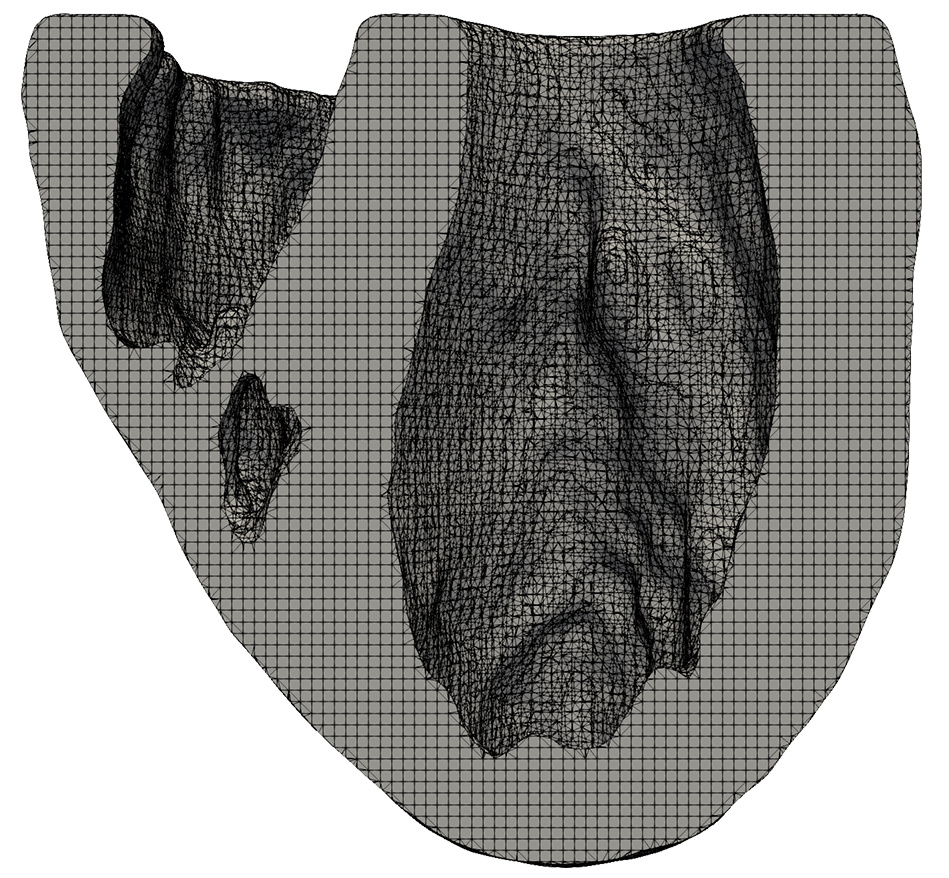
\includegraphics[scale=0.15]{media/3-celeris/8-celeris.png}
\label{fig:comp-1}}		
\subfigure[]{%
		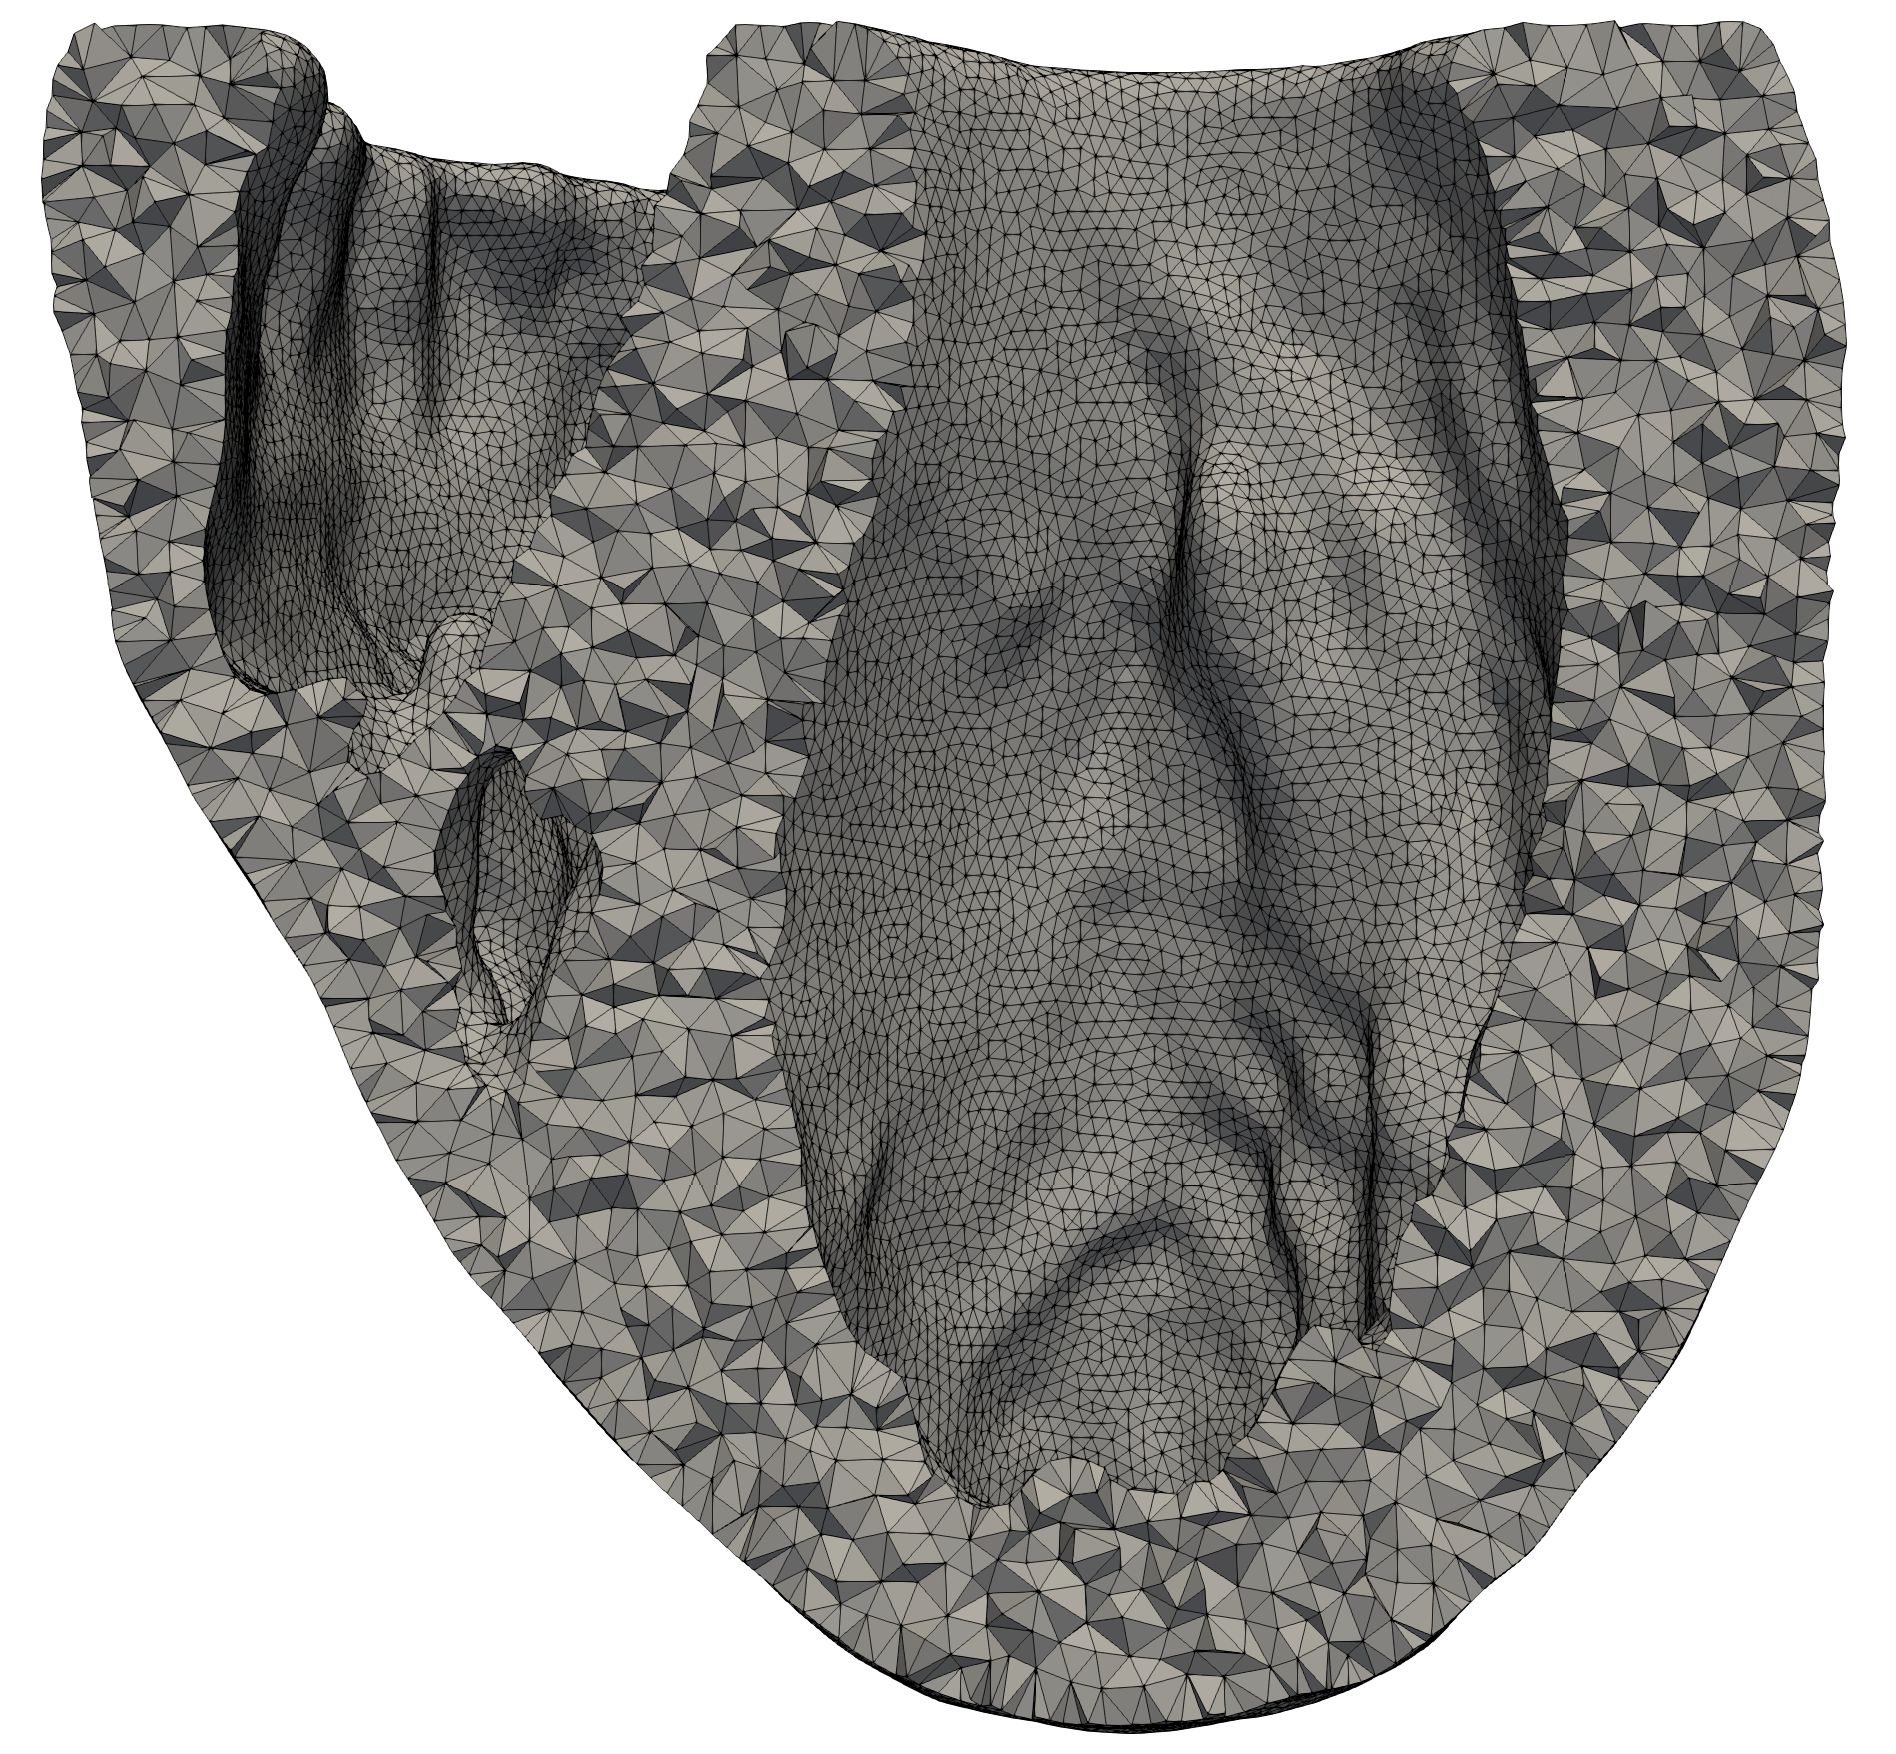
\includegraphics[scale=0.15]{media/3-celeris/9-cardioid.png}		
\label{fig:comp-2}}	
\subfigure[]{%
		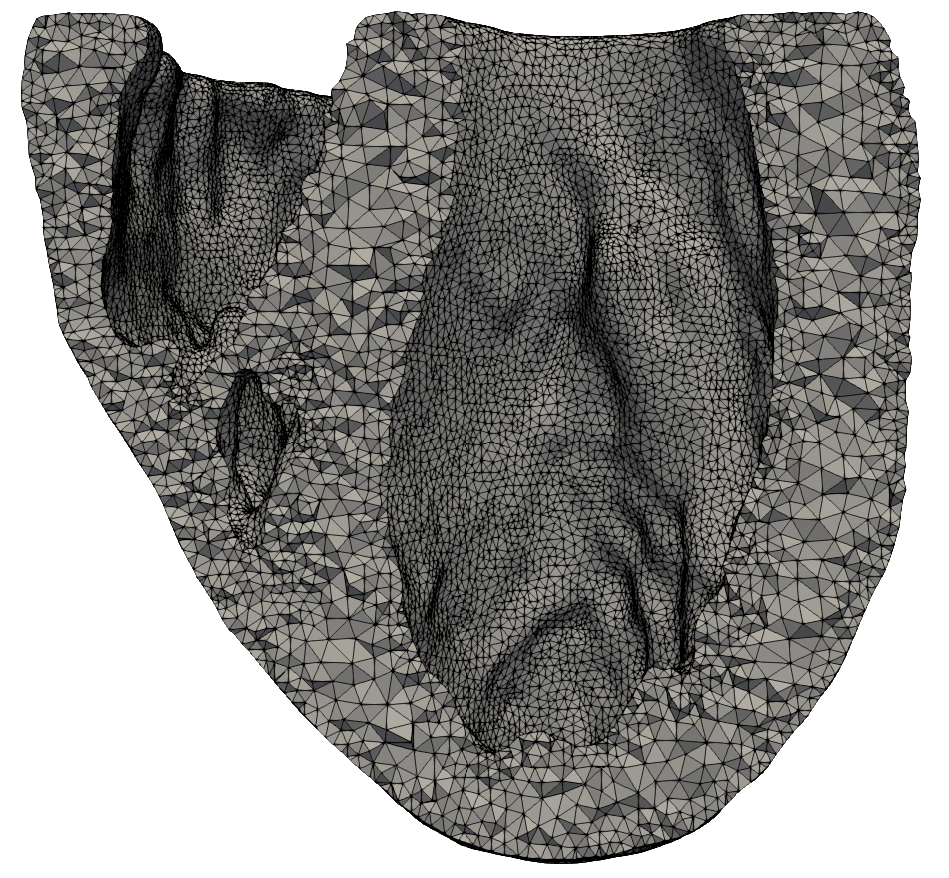
\includegraphics[scale=0.15]{media/3-celeris/10-simpleware.png}
\label{fig:comp-3}}			
	
%
\caption{Comparison of meshes: (a) linear polyhedral mesh from Celeris, (b) quadratic tetrahedral mesh from Tetgen, (c) and quadratic tetrahedral mesh from Simpleware.}
\label{fig:comp}
\end{figure}

{http://www.springer.com/us/book/9781441907295} \\
Cardioid science on saturday Youtube
$heart_papers$
papers Mark mentions in SOW

%%%%%%%%%%%%%%%%%%%%%%%%%%%%%%%%%%%%%%%%%%%%%%%
%%%%%%%%%%%%%%%%%%%%%%%%%%%%%%%%%%%%%%%%%%%%%%%
\section{Description of Cardioid}
\label{Description of Cardioid}

%%%%%%%%%%%%%%%%%%%%%%%%%%%%%%%%%%%%%%%%%%%%%%%
%%%%%%%%%%%%%%%%%%%%%%%%%%%%%%%%%%%%%%%%%%%%%%%
\section{Material Property Characterization}
\label{Material Property Characterization}

%%%%%%%%%%%%%%%%%%%%%%%%%%%%%%%%%%%%%%%%%%%%%%%
%%%%%%%%%%%%%%%%%%%%%%%%%%%%%%%%%%%%%%%%%%%%%%%
\section{Fiber Generation}
\label{Simulation}

%%%%%%%%%%%%%%%%%%%%%%%%%%%%%%%%%%%%%%%%%%%%%%%
%%%%%%%%%%%%%%%%%%%%%%%%%%%%%%%%%%%%%%%%%%%%%%%
\section{Boundary Conditions}
\label{Boundary Conditions}

%%%%%%%%%%%%%%%%%%%%%%%%%%%%%%%%%%%%%%%%%%%%%%%
%%%%%%%%%%%%%%%%%%%%%%%%%%%%%%%%%%%%%%%%%%%%%%%
\section{Simulation/Results}
\label{Simulation/Results}


Questions to ask with available model
Effect of smoothing/trabeculae
Do trabeculae affect the solution
How sensitive are the results from paraview smoothing?
Effect of resolution – make multiple meshes of same geometry
Number of iterations – do they depend on mesh resolution? Would like it not to 
Does V cycle work for my geometry?
Fiber generation vs fibers from raw data + interp + smoothing
Verification/validation
Stress/strain plots
Initial cycle is faster than others: first frame but also first cycle all together is faster
Mesh quality/aspect ratio
Potential plots:	
Volumetric strain
Deviatoric strain
C11, c22, c33
Maximal principal eigenvalue
C11 from fiber orientation
Hysteresis plot of position

structure/trabeculae
fibergen vs DTI
Jeremy drug studies, a lot didn’t match
whole range of sensitivity studies



­Preliminary Ideas

How does fiber orientation impact lengthening of heart
How does mesh resolution affect solution
Explore exotic solvers
Complete tool chain
How does constitutive and active properties of heart affect solution


Nearly incompressible material leads to poor condition number in stiffness matrix
Want to study how large scale, iterative solvers can be formulated to deal with poor condition number, as well as interact with element shape and mesh quality
Want to couple electrophysiology model with mechanics model
Want to understand the impact of mesh quality on solver performance, and help tune mesh generation procedures to generate meshes that are free of features that cause problems for the solver
Why is full model not performing as well? Active tension, anisotropy, geometry. Which is the one that makes it hard?


Solver may struggle due to a few elements that have a weird shape (Mesquite), meshing is a problem
Activation model
Coupling of electrophysiological and mechanical model (feedback may not be important)
Electrophysiology model scales much larger than mechanical model, and can be solved almost real time
Couple electrophysiology to ECG code – finite element locations fed into ECG (same code base as FEM code)
What parameters are affecting the result?
Develop tool chain – sensitivity analysis





What does it mean exactly to have an active component of stress? basically just a body force
The ventricles are coupled to a lumped circulatory model? Volume as a function of time
Direct solvers used because of active force component (?)
Direct solvers limit number of DOF
This method suggested is a Krylov subpace iterative solver, increases number of DOF, much larger scale problem
 Why quasi-static?? Elastic portion reacts very quickly
Any reason why quadratic elements chosen as opposed to linear elements? Avoid volumetric locking
“The main reason why the mixed displacement-pressure formulation for incompressible large deformation problems is often avoided is the difficulty in solving such saddle-point linear systems, and this difficulty is increased by the presence of active stress.”
“problems with pyramid element” – why problems? Even after 15 node element introduced?


winslow canine diffusion tensor segmentation


Mark Rashid meeting

~ important to have every day workhorse stable analysis tool available

~ may be getting oscillations in pressure field that are hard to avoid in current formulation

~ oscillations in displacement from bending in beam is concerning - issue with constitutive model

~ near-incompressibility instead of fully incompressible

instead of pressure formulation, all displacement, only nearly enforce incompressibility
element-wide average of element dilatation, essentially reduced-integration, a remedy for locking
enhanced assumed strain / enhanced kinematics
much more common to do all displacement, enhance kinematics instead of pressure formulation

~ BCs: projecting out rigid body translations and rotations

~ before today, the three options were fully tet, fully hex, and mixed. can we reiterate why you wouldn’t recommend any of those three and why you would instead recommend polyhedral FEM laid out today

~ in the same way you have biological and electrophysiology experts, only makes sense to have an expert in computational solid mechanics

---------------------------------------

~ tets not okay - too many DOFs, accuracy potentially worse, even for higher order
~ full hex mesh nearly impossible
~ mixed element: somewhere in between. prisms and pyramids are algorithmically difficult. Also, issues with convergence



Prof Rashid’s suggestions

direct solver instead of iterative solver
is fiber discontinuity interacting with incompressibility constraint?
1 for experimentation, play with compressible passive formulation
2 take incompressibility off the table
three main differences: geometry, continuous fiber orientations, purely tet
mixture of elements could cause problems with convergence

WHAT CAN WE BE SLOPPY ABOUT? WHICH PARAMETERS MOST IMPORTANTLY AFFECT THE RESULT?


---

Natalia Trayanova is not the only one simulating beating hearts.

Some other profs that simulate beating hearts ...

Andrew McCulloch:
http://cmrg.ucsd.edu/AndrewMcCulloch

Steve Niederer
kclpure.kcl.ac.uk/portal/steven.niederer.html

Blanca Rodriguez
www.cs.ox.ac.uk/people/blanca.rodriguez